% !TEX root = Tesi.tex
              %******************************************%
              %                                          %
              % Template standard per la Tesi di Laurea  %
              %            di Stefano Bianchi            %
              %                                          %
              %         versione: 27 marzo 2014          %
              %                                          %
              %******************************************%

% Se si vuole stampare su entrambi i lati, porre la dicitura 'twoside'
% tra i parametri documentclass
\documentclass[a4paper,11pt,oneside,openany]{book}

\usepackage[english,italian]{babel}

\usepackage[utf8]{inputenc}
\usepackage[T1]{fontenc}
\usepackage{lmodern}

\usepackage{fancyhdr}
\usepackage{graphicx}
\usepackage{subfigure}
\usepackage{tabularx}
\usepackage{longtable}
\usepackage{float}
\usepackage{fancyvrb}
\usepackage{amsmath}
\numberwithin{equation}{section}
\usepackage{hyperref}

\usepackage{geometry}
\usepackage{textcomp}
\usepackage{color}
\usepackage{xspace}

\usepackage{amssymb,amsfonts}
\usepackage{booktabs}
\usepackage{siunitx}
\usepackage{algorithm}
\usepackage{algpseudocode}
\floatname{algorithm}{Algoritmo}
\renewcommand{\algorithmicrequire}{\textbf{Ingresso:}}
\renewcommand{\algorithmicensure}{\textbf{Uscita:}}
\renewcommand{\algorithmicfor}{\textbf{per}}
\renewcommand{\algorithmicforall}{\textbf{per ogni}}
\renewcommand{\algorithmicdo}{\textbf{esegui}}
\renewcommand{\algorithmicend}{\textbf{fine}}
\renewcommand{\algorithmicif}{\textbf{se}}
\renewcommand{\algorithmicthen}{\textbf{allora}}
\renewcommand{\algorithmicreturn}{\textbf{restituisci}}
\usepackage{paralist}
\usepackage[inline]{enumitem}
\usepackage{xcolor}
\usepackage{array}

\definecolor{codegreen}{rgb}{0,0.6,0}
\definecolor{codegray}{rgb}{0.5,0.5,0.5}
\definecolor{codeblue}{rgb}{0,0,225}
\definecolor{codepurple}{HTML}{C42043}
\definecolor{backcolour}{HTML}{F2F2F2}
\definecolor{bookColor}{cmyk}{0,0,0,0.90}
\color{bookColor}

\makeatletter
\def\namedlabel#1#2{\begingroup
   \def\@currentlabel{#2}%
   \phantomsection\label{#1}\endgroup
}
\makeatother

%*******************************************************
% Impostazioni della singola pagina e della copertina
%*******************************************************
\hypersetup{ % Visualizzazione dei collegamenti cliccabili
    colorlinks,
    citecolor=black,
    filecolor=black,
    linkcolor=black,
    urlcolor=black
}

% Imposta l'intestazione delle pagine
\setlength{\headheight}{13.6pt}    % richiesto da fancyhdr
\addtolength{\topmargin}{-1.6pt}   % compensa l'aumento di headheight
\fancyhf{}
\pagestyle{fancy}
\lhead{}
\chead{\leftmark}
\rhead{}
\lfoot{}
\cfoot{}
\rfoot{\thepage}

\usepackage[square, comma, numbers]{natbib}
\usepackage{xcolor}

\setlength{\parindent}{0pt}
\usepackage[italian]{cleveref}
\crefname{algorithm}{algoritmo}{algoritmi}
\Crefname{algorithm}{Algoritmo}{Algoritmi}
\usepackage{verbatim}
\usepackage{amsmath}

% Note a margine per bozza (usato come TODO nel testo)
\newcommand{\mnote}[1]{\marginpar{\footnotesize\color{red} #1}}


%*******************************************************
% Copertina
%*******************************************************
% Non modificare questa parte
\usepackage[some]{background}
\SetBgScale{1}
\SetBgContents{

\includegraphics[scale=1]{img/units.png}}
\SetBgColor{gray}
\SetBgAngle{0}
\SetBgOpacity{0.07}
% Non modificare questa parte

% Titolo della tesi e autore
\title{Donazioni di sangue nelle province di Trieste e Gorizia dal 2009 al 2025: analisi dei dati e studio sul futuro}
\author{Marco Secci}
% Senza questo i metadati del PDF restano vuoti: \title e \author da soli
% popolano il frontespizio, non le proprieta' del file.
\hypersetup{pdftitle={Donazioni di sangue nelle province di Trieste e Gorizia dal 2009 al 2025: analisi dei dati e studio sul futuro},
            pdfauthor={Marco Secci}}
\begin{document}
\pagenumbering{roman}
\begin{titlepage}
    \begin{center}
    % Insert the background here (front page)
    %\BgThispage
    {\LARGE {\bfseries UNIVERSIT\`A DEGLI STUDI DI TRIESTE \\}}
    \vspace{.5cm}
    {\Large {\bfseries Dipartimento di Matematica, Informatica e Geoscienze. \\}}
    \vspace{1cm}
    
\includegraphics[width=6cm,height=6cm]{img/units.png}\\[1.5cm]
    {\centering
        {\LARGE
        Laurea Triennale \\ in Intelligenza Artificiale e Data Analytics \\
        }\par
    }
    \vspace{1cm}
    {\LARGE 
        {\bfseries Donazioni di sangue nelle province di Trieste e Gorizia dal 2009 al 2025: analisi dei dati e studio sul futuro}
    }
    \vspace{1cm}

    % Ricordarsi di aggiornare la data prima di inviare in stampa il documento :)
    {\large % Ricordarsi di aggiornare la data prima di inviare in stampa il documento :)
{\large 1 ottobre 2026 \\
}
    }

    % Tabella per inserire i nomi del laureando, del relatore e dell'eventuale correlatore nel modo migliore all'interno della pagina
    \vfill
    \begin{table}[h]
        {\large
            \begin{tabular}{c c c c r c c | c c l}
                & & & & Laureando & & & & & Relatore \\
                & & & & \bfseries Marco Secci & & & & & \bfseries Leonardo Egidi \\ % Modificare il nome del laureando
                & & & & & & & & & \\
                & & & & & & & & & Correlatore \\ % Nel caso in cui non si ha il correlatore,
                & & & & & & & & & \bfseries Massimo La Raja \\ % eliminare queste due righe
            \end{tabular}
        }
    \end{table}
    A. A. 2025/2026
        \end{center}
\end{titlepage}


%*******************************************************
% Dedica
%*******************************************************
% Non modificare questa parte
\phantomsection
\thispagestyle{empty}
\vspace*{3cm}
% Non modificare questa parte
Ai miei mici Pedro e Yuki, che con i loro miagolii e le loro fusa hanno reso ogni giorno unico.

\frontmatter

%*******************************************************
% Sommario
%*******************************************************
\chapter{Sommario}

Il sistema trasfusionale non può produrre ciò che distribuisce: sangue, plasma
e piastrine dipendono per intero dalla disponibilità volontaria dei donatori.
Capire chi dona, con quale frequenza e per quanti anni continua a farlo è
quindi una premessa operativa alla programmazione della raccolta.
Questa tesi affronta la domanda su dati reali:
l'archivio donazionale del \textbf{Dipartimento Interaziendale di Medicina
Trasfusionale (DIMT)} di Trieste e Gorizia, due province del Friuli Venezia
Giulia con popolazione mediamente più anziana del resto del Paese e una rete
associativa particolarmente radicata.

Il lavoro parte da 27 file Excel eterogenei per schema e convenzioni di
denominazione e li riconduce, attraverso una pipeline in Python documentata in
ogni suo stadio, a un unico dataset analitico di \textbf{353\,671 eventi di
donazione} riferiti a \textbf{43\,299 donatori distinti} nel periodo
\textbf{2009--2025}. Su questa base sono condotte quattro analisi:
un'esplorazione descrittiva della popolazione donante e delle sue tendenze
temporali, rapportate per la prima volta alla popolazione residente; uno studio
di fidelizzazione condotto per coorte di ingresso; una proiezione del volume
donazionale al 2031 selezionata con un backtest a origine mobile fra diciassette
modelli candidati; e un modello di regressione per dati di conteggio sulla
frequenza donazionale individuale. I risultati sono infine resi ispezionabili
in una dashboard interattiva in R Shiny.

Il quadro che emerge è quello di un sistema in contrazione lenta e continua. Il
volume annuale cala del \textbf{28{,}1\%} fra il 2009 e il 2025, concentrando
la flessione nella prima metà del periodo per poi assestarsi; i nuovi ingressi
calano di più; e l'intensità individuale --- il numero di donazioni per
donatore attivo --- resta invariata fra $1{,}84$ e $1{,}97$ lungo tutti e
diciassette gli anni. Il sistema, cioè, non si è intensificato per compensare
il minor ricambio: si è ridotto e poi assestato su una base più piccola, anche grazie
al calo dei consumi.

Rapportare le donazioni alla popolazione residente di Trieste e Gorizia separa
ciò che è demografia da ciò che è comportamento, e il risultato non è quello
che ci si aspetterebbe. Il calo della popolazione in età donabile spiega solo
il \textbf{12{,}2\%} della contrazione; quasi tutto il resto è perdita di
partecipazione vera, da $106{,}9$ a $80{,}1$ donazioni ogni mille residenti. E
la perdita non è dove la
si cercherebbe: a parità di popolazione i \textbf{20--24enni sono la fascia con
il tasso di donazione più alto in ogni anno osservato}, mentre le fasce 35--44
perdono fra il 36 e il 41 per cento. Il problema dei giovani non è che non
cominciano --- sono la metà di tutti gli ingressi --- ma che non tornano: il
\textbf{40{,}6\%} non si ripresenta dopo la prima donazione, contro il
$33{,}3\%$ di chi entra più tardi, e la funzione di rischio decrescente
individua una soglia di consolidamento dell'abitudine intorno al terzo--quinto
anno.

Il modello di frequenza mostra che gli effetti dominanti sono di natura
regolamentare più che motivazionale (genere, IRR $0{,}585$; plasmaferesi, IRR
$1{,}77$: intervalli minimi e tetti annui differenziati) e che, controllando
per gli anni di carriera, \textbf{l'età anagrafica non ha alcun effetto}: ciò
che distingue un donatore assiduo è da quanto tempo dona, non quanti anni ha.
Coerentemente, le proiezioni indicano per il sessennio 2026--2031 circa
\textbf{97\,200 donazioni} complessive: un primo anno sensibilmente sotto il
2025, poi una contrazione di poco meno di un punto percentuale l'anno, senza
ricomposizione attesa fra tipologie. Un assottigliamento lento, non una
rottura.


\begin{otherlanguage}{english}
\chapter{Abstract}

A transfusion system cannot manufacture what it distributes: blood, plasma
and platelets depend entirely on donors coming forward voluntarily.
Knowing who donates, how often and for how many years is therefore an
operational prerequisite for planning collection.
This thesis addresses the question with real data:
the donation records of the \textbf{Interhospital Department of Transfusion
Medicine (DIMT)} of Trieste and Gorizia, two provinces of Friuli Venezia
Giulia whose population is older on average than the rest of Italy and whose
donor associations are particularly well established.

The work starts from 27 Excel files with inconsistent schemas and naming
conventions and, through a Python pipeline documented at every stage, merges
them into a single analytical dataset of \textbf{353\,671 donation events}
from \textbf{43\,299 distinct donors} over \textbf{2009--2025}. Four analyses
are built on it: a descriptive exploration of the donor population and its
trends over time, related for the first time to the resident population; a
retention study by entry cohort; a projection of donation volume to 2031,
selected through a rolling-origin backtest among seventeen candidate models; and
a count regression model of individual donation frequency. The results are
also made explorable in an interactive R Shiny dashboard.

The picture is one of slow, steady contraction. Annual volume falls by
\textbf{28.1\%} between 2009 and 2025, with most of the decline in the first
half of the period before it levels off; new entries fall even more; and
individual intensity --- donations per active donor --- stays between $1.84$
and $1.97$ across all seventeen years. The system, in other words, did not
intensify to make up for lower turnover: it shrank and then settled on a
smaller base, helped in part by falling demand.

Relating donations to the resident population of Trieste and Gorizia separates
demography from behaviour, and the result is not what one would expect. The
decline in the population of eligible age explains only \textbf{12.2\%} of the
contraction; nearly all the rest is a genuine loss of participation, from
$106.9$ to $80.1$ donations per thousand residents. Nor is the loss where one
would look for it: relative to population, \textbf{people aged 20--24 have the
highest donation rate in every year observed}, while the 35--44 age groups
lose between 36 and 41 per cent. The problem with young donors is not that
they fail to start --- they account for half of all entries --- but that they
do not come back: \textbf{40.6\%} never return after their first donation,
against $33.3\%$ of those who start later, and the decreasing hazard function
points to a threshold around the third to fifth year at which the habit
consolidates.

The frequency model shows that the dominant effects are regulatory rather than
motivational (sex, IRR $0.585$; plasmapheresis, IRR $1.77$: different minimum
intervals and annual caps) and that, once years of donor career are controlled
for, \textbf{age has no effect at all}: what sets a frequent donor apart is how
long they have been donating, not how old they are. Consistently, the
projections point to about \textbf{97\,200 donations} in total over 2026--2031: a first
year clearly below 2025, then a contraction of just under one percentage point
a year, with no expected shift in the mix of donation types. A slow thinning,
not a break.

\end{otherlanguage}


%*******************************************************
% Indice
%*******************************************************
\tableofcontents

%*******************************************************
% Introduzione
%*******************************************************
% Non modificare questa parte
\renewcommand{\chaptermark}[1]{\markboth{\MakeUppercase{\ #1}}{}}
% Non modificare questa parte

\chapter{Introduzione}

La donazione di sangue è un atto volontario e altruistico che costituisce uno
dei pilastri del sistema sanitario moderno. Il sangue, come piastrine e plasma,
non sono sostanze sintetizzabili artificialmente in laboratorio: 
la loro disponibilità dipende in modo esclusivo dalla scelta dei cittadini di donare.
In Italia il sistema trasfusionale si regge su una rete capillare di associazioni di 
volontariato e su centri ospedalieri regionali che gestiscono raccolta, lavorazione e
distribuzione degli emocomponenti.

Il Friuli Venezia Giulia presenta, nel suo insieme, caratteristiche degne di
nota per le analisi che seguiranno: una popolazione mediamente anziana (48,8 anni,
1,7 in più della media nazionale~\cite{etàmediaFVG}) e una forte presenza di
volontariato. Il presente lavoro, tuttavia, non copre l'intera regione. In Friuli Venezia
Giulia operano tre Dipartimenti Interaziendali di Medicina Trasfusionale,
ciascuno dei quali fa riferimento ad un territorio specifico, gestendo
le operazioni di donazione e raccolta tra presidi ospedalieri principali e 
autoemoteche che operano nei comuni minori:
quello dell'Azienda Sanitaria Universitaria Giuliano Isontina (ASUGI), 
competente su Trieste e Gorizia; quello
dell'Azienda Sanitaria Universitaria Friuli Centrale (ASUFC), su Udine; e
quello dell'Azienda Sanitaria Friuli Occidentale (ASFO), su Pordenone. I dati
disponibili per questo lavoro sono quelli del \textbf{DIMT dell'ASUGI}.

Le province di Trieste e Gorizia rappresentano circa un quinto del bacino
donazionale regionale e non ne riproducono le caratteristiche: la realtà
sociale ed economica dell'area giuliano-isontina, e in particolare del
capoluogo triestino, si differenzia per molti aspetti --- demografici,
economici e organizzativi --- da quella di Udine e Pordenone. Le conclusioni
di questo lavoro vanno perciò lette come relative al territorio
effettivamente osservato, e non estese senza verifica al resto della regione.

Comprendere i fattori che influenzano la frequenza e la continuità delle
donazioni è rilevante sia sul piano scientifico sia su quello operativo:
permette di identificare i profili a rischio di abbandono, di pianificare
campagne di reclutamento mirate e di anticipare fluttuazioni nell'offerta di
emocomponenti. Il presente lavoro approfondisce questi aspetti analizzando un
dataset longitudinale di \textbf{diciassette anni} di attività donazionale
nelle province di Trieste e Gorizia, dal 2009 al 2025, con strumenti di
statistica descrittiva e di modellazione regressiva.

Una precisazione di metodo, perché orienta la lettura di tutto ciò che segue.
Il calo delle donazioni è un fatto noto e ripetutamente osservato; è invece
raramente scomposto. Un sistema che raccoglie meno sangue in un territorio che
perde abitanti può essere in erosione oppure semplicemente più piccolo, e le
due diagnosi portano a decisioni opposte. Il \cref{ch:eda} affronta la
distinzione esplicitamente, rapportando le donazioni alla popolazione
residente, e il risultato che ne esce condiziona la lettura dei capitoli
successivi.

Il contributo della tesi è duplice. Sul piano applicativo, quantifica per le
province di Trieste e Gorizia un fenomeno spesso descritto solo
qualitativamente e ne individua i punti
di intervento --- la prima ripetizione dei donatori giovani e il rientro della
fascia di mezza età --- laddove il margine sui donatori già attivi risulta
invece vincolato in alto da regole cliniche. Sul piano metodologico, mostra che
tre scelte apparentemente tecniche cambiano le conclusioni: quale colonna
identifica il donatore, se un campo amministrativo incompleto sia un requisito
o una covariata, e su quale unità di analisi si misuri un conteggio. Ogni
figura e ogni numero riportati sono tracciabili al comando che li ha prodotti.

%*******************************************************
% Capitoli
%*******************************************************
\mainmatter

% Non modificare questa parte
\renewcommand{\chaptermark}[1]{\markboth{\MakeUppercase{\chaptername\ \thechapter.\ #1}}{}}
% Non modificare questa parte

% ══════════════════════════════════════════════════════════════════════════════
%  CAPITOLO — DATI E COSTRUZIONE DEL DATASET
%  Etichette: ch:data, sec:rawdata, sec:decisioni, sec:cleaning, sec:phaselog,
%             sec:dataset, sec:datasummary
%             tab:files, tab:colmap, tab:nulli_sede, tab:cleaninglog, tab:columns
% ══════════════════════════════════════════════════════════════════════════════

\chapter{Dati originali e Costruzione del Dataset}
\label{ch:data}

Il presente capitolo descrive il materiale empirico su cui poggia l'intero
elaborato: la provenienza e la struttura dei file grezzi forniti dal
Dipartimento Interaziendale di Medicina Trasfusionale (DIMT) di Trieste e
Gorizia, e la pipeline che li riconduce a un unico dataset analitico. Due
scelte, in particolare, condizionano tutto ciò che segue --- quale colonna
identifica il donatore e come si trattano i valori mancanti --- e vengono
discusse per esteso, perché è da lì che dipende quanto dato arriva alle analisi.

% L'obiettivo è duplice: rendere \textbf{riproducibile} ogni passaggio e separare
% nettamente la costruzione del dataset dal \Cref{ch:eda}, dove a partire dal
% file finale si presenta la prima descrizione quantitativa della popolazione
% donante.

% ───────────────────────────────────────────────────────────────────────
\section{Fonti dei dati grezzi}
\label{sec:rawdata}

I dati sono stati forniti dal DIMT come archivio di fogli di calcolo Microsoft
Excel (\texttt{.xlsx}), suddivisi per anno e, in alcuni casi, per sotto-area
territoriale (sedi isontine, autoemoteche) o per semestre. I file coprono in
modo continuo il periodo \textbf{2009--2025}; complessivamente sono stati
elaborati \textbf{27 file sorgente} (\cref{tab:files}), per un totale di
\textbf{370\,552 righe}.

\begin{table}[ht]
\centering
\caption{Schema di organizzazione dei file sorgente. Le diciture sono
semplificate; i pattern esatti dei nomi possono variare.}
\label{tab:files}
\small
\setlength{\tabcolsep}{4pt}
\begin{tabular}{@{}lll@{}}
\toprule
\textbf{Periodo} & \textbf{Pattern del file} & \textbf{Note} \\
\midrule
2009--2017 & \texttt{YYYY DIMT TOT S.xlsx} o          & un file per anno \\
           & \texttt{AI DIMT YYYY TOT S.xlsx}         &  \\
2018--2020 & \texttt{AI DIMT YYYY TOT S.xlsx}\,$+$    & file aggiuntivo \\
           & \texttt{AI DIMT YYYY CURPE ISONTINO S.xlsx} & per le sedi isontine \\
2021--2022 & \texttt{F DIMT YYYY \ldots.xlsx}         & tracciato ridotto \\
2023       & \texttt{2023 tot dimt new.xlsx}\,$+$     & due estrazioni dello \\
           & \texttt{2023 ADS Emoteca new.xlsx}       & stesso insieme di eventi \\
2024       & \texttt{2024 DIMT TOT S.xlsx}\,$+$       & quattro file aggiuntivi \\
           & \texttt{AI 2024 CURPE ISONTINO \ldots.xlsx} & per le sedi isontine \\
2025       & \texttt{DIMT 2025 1\textsuperscript{o}\,SEM TOT.xlsx}\,$+$ & raccolta semestrale \\
           & \texttt{DIMT 2025 2\textsuperscript{o}\,SEM TOT.xlsx}\,$+$ &  \\
           & \texttt{AE 2025.xlsx}                    & autoemoteche separate \\
\bottomrule
\end{tabular}
\end{table}

Ogni riga rappresenta un singolo \emph{evento di donazione}: vi sono codificate
informazioni anagrafiche minime (sesso, data di nascita, età al momento della
donazione), informazioni amministrative (classe del donatore, associazione di
appartenenza, punto di raccolta, data di inizio attività) e informazioni
specifiche dell'evento (tipo di donazione, quantità in mL, data). Il donatore
non è identificato da un dato anagrafico diretto ma da un codice (\texttt{crd})
già pseudonimizzato alla fonte dal DIMT. L'utilizzo di questo archivio per la
presente tesi è stato concordato con il Responsabile della Protezione dei Dati
(DPO) dell'ASUGI: la condizione posta riguardava la riduzione al minimo dei
dati personali trattati e un adeguato livello di anonimizzazione o
pseudonimizzazione, a cui il dataset analitico si attiene limitandosi alle
colonne elencate in \cref{tab:colmap} e scartando ogni altro campo
amministrativo non necessario alle analisi.

Le intestazioni di colonna non sono omogenee fra anni: la colonna dell'età
compare come \texttt{ETA}, \texttt{ETA'} o \texttt{Eta\_anni}, quella delle
quantità come \texttt{qta\_ml} o \texttt{quantita\_ml}. Il primo stadio della
pipeline le riconcilia su un unico schema (\cref{tab:colmap}); una colonna
sconosciuta interrompe l'elaborazione anziché essere ignorata in silenzio, così
che un file con una convenzione nuova si faccia notare.

\begin{table}[ht]
\centering
\caption{Mappatura delle colonne dai nomi originali a quelli standardizzati.
Sono riportate le colonne effettivamente usate nelle analisi.}
\label{tab:colmap}
\small
\setlength{\tabcolsep}{4pt}
\begin{tabular}{@{}lll@{}}
\toprule
\textbf{Nome originale} & \textbf{Nome standardizzato} & \textbf{Descrizione} \\
\midrule
\texttt{crd}                  & \texttt{donor\_id}            & Identificativo anonimo donatore \\
\texttt{id\_anag}             & \texttt{donor\_id\_anag}      & Identificativo alternativo (controllo) \\
\texttt{dtatt\_da}            & \texttt{donation\_datetime}   & Data e ora dell'evento \\
\texttt{descr\_breve\_emcdon} & \texttt{donation\_type}       & Tipo di donazione \\
\texttt{dtinizatt\_da}        & \texttt{first\_activity\_date}& Data di inizio attività donazionale \\
\texttt{class\_don}           & \texttt{donor\_class}         & Classe donatore (P, O, D, A) \\
\texttt{s}                    & \texttt{sex}                  & Sesso \\
\texttt{nascita}              & \texttt{birth\_date}          & Data di nascita \\
\texttt{eta}                  & \texttt{age}                  & Età alla donazione \\
\texttt{qta}                  & \texttt{quantity\_ml}         & Quantità donata nell'evento (mL) \\
\texttt{num\_don}             & \texttt{num\_don\_declared}   & Conteggio dichiarato (controllo) \\
\texttt{qta\_tot}             & \texttt{quantity\_total\_ml}  & Quantità cumulativa (controllo) \\
\texttt{descr\_pdr}           & \texttt{collection\_point}    & Punto di raccolta \\
\texttt{descrizione\_ass}     & \texttt{association\_desc}    & Nome associazione \\
\texttt{validita}             & \texttt{validity}             & Validità della donazione \\
\bottomrule
\end{tabular}
\end{table}

L'eterogeneità non riguarda solo i nomi: cambia anche \emph{quali} colonne
esistono. La \cref{fig:null_heatmap} lo rende visibile in un colpo d'occhio ---
è costruita sui nomi grezzi, perché è del dato grezzo che parla. Alcune colonne
compaiono solo in anni isolati e recenti (\texttt{section\_code},
\texttt{validity}: 2023 e 2025), altre spariscono nel triennio 2021--2023,
quando i file cambiano formato e si riducono, in gran parte del triennio, a
otto colonne. Una colonna assente per quindici anni su diciassette non può
fare da criterio di filtro sull'intero periodo: è l'osservazione da cui
discende tutta la \cref{sec:decisioni}.

\begin{figure}[H]
    \centering
    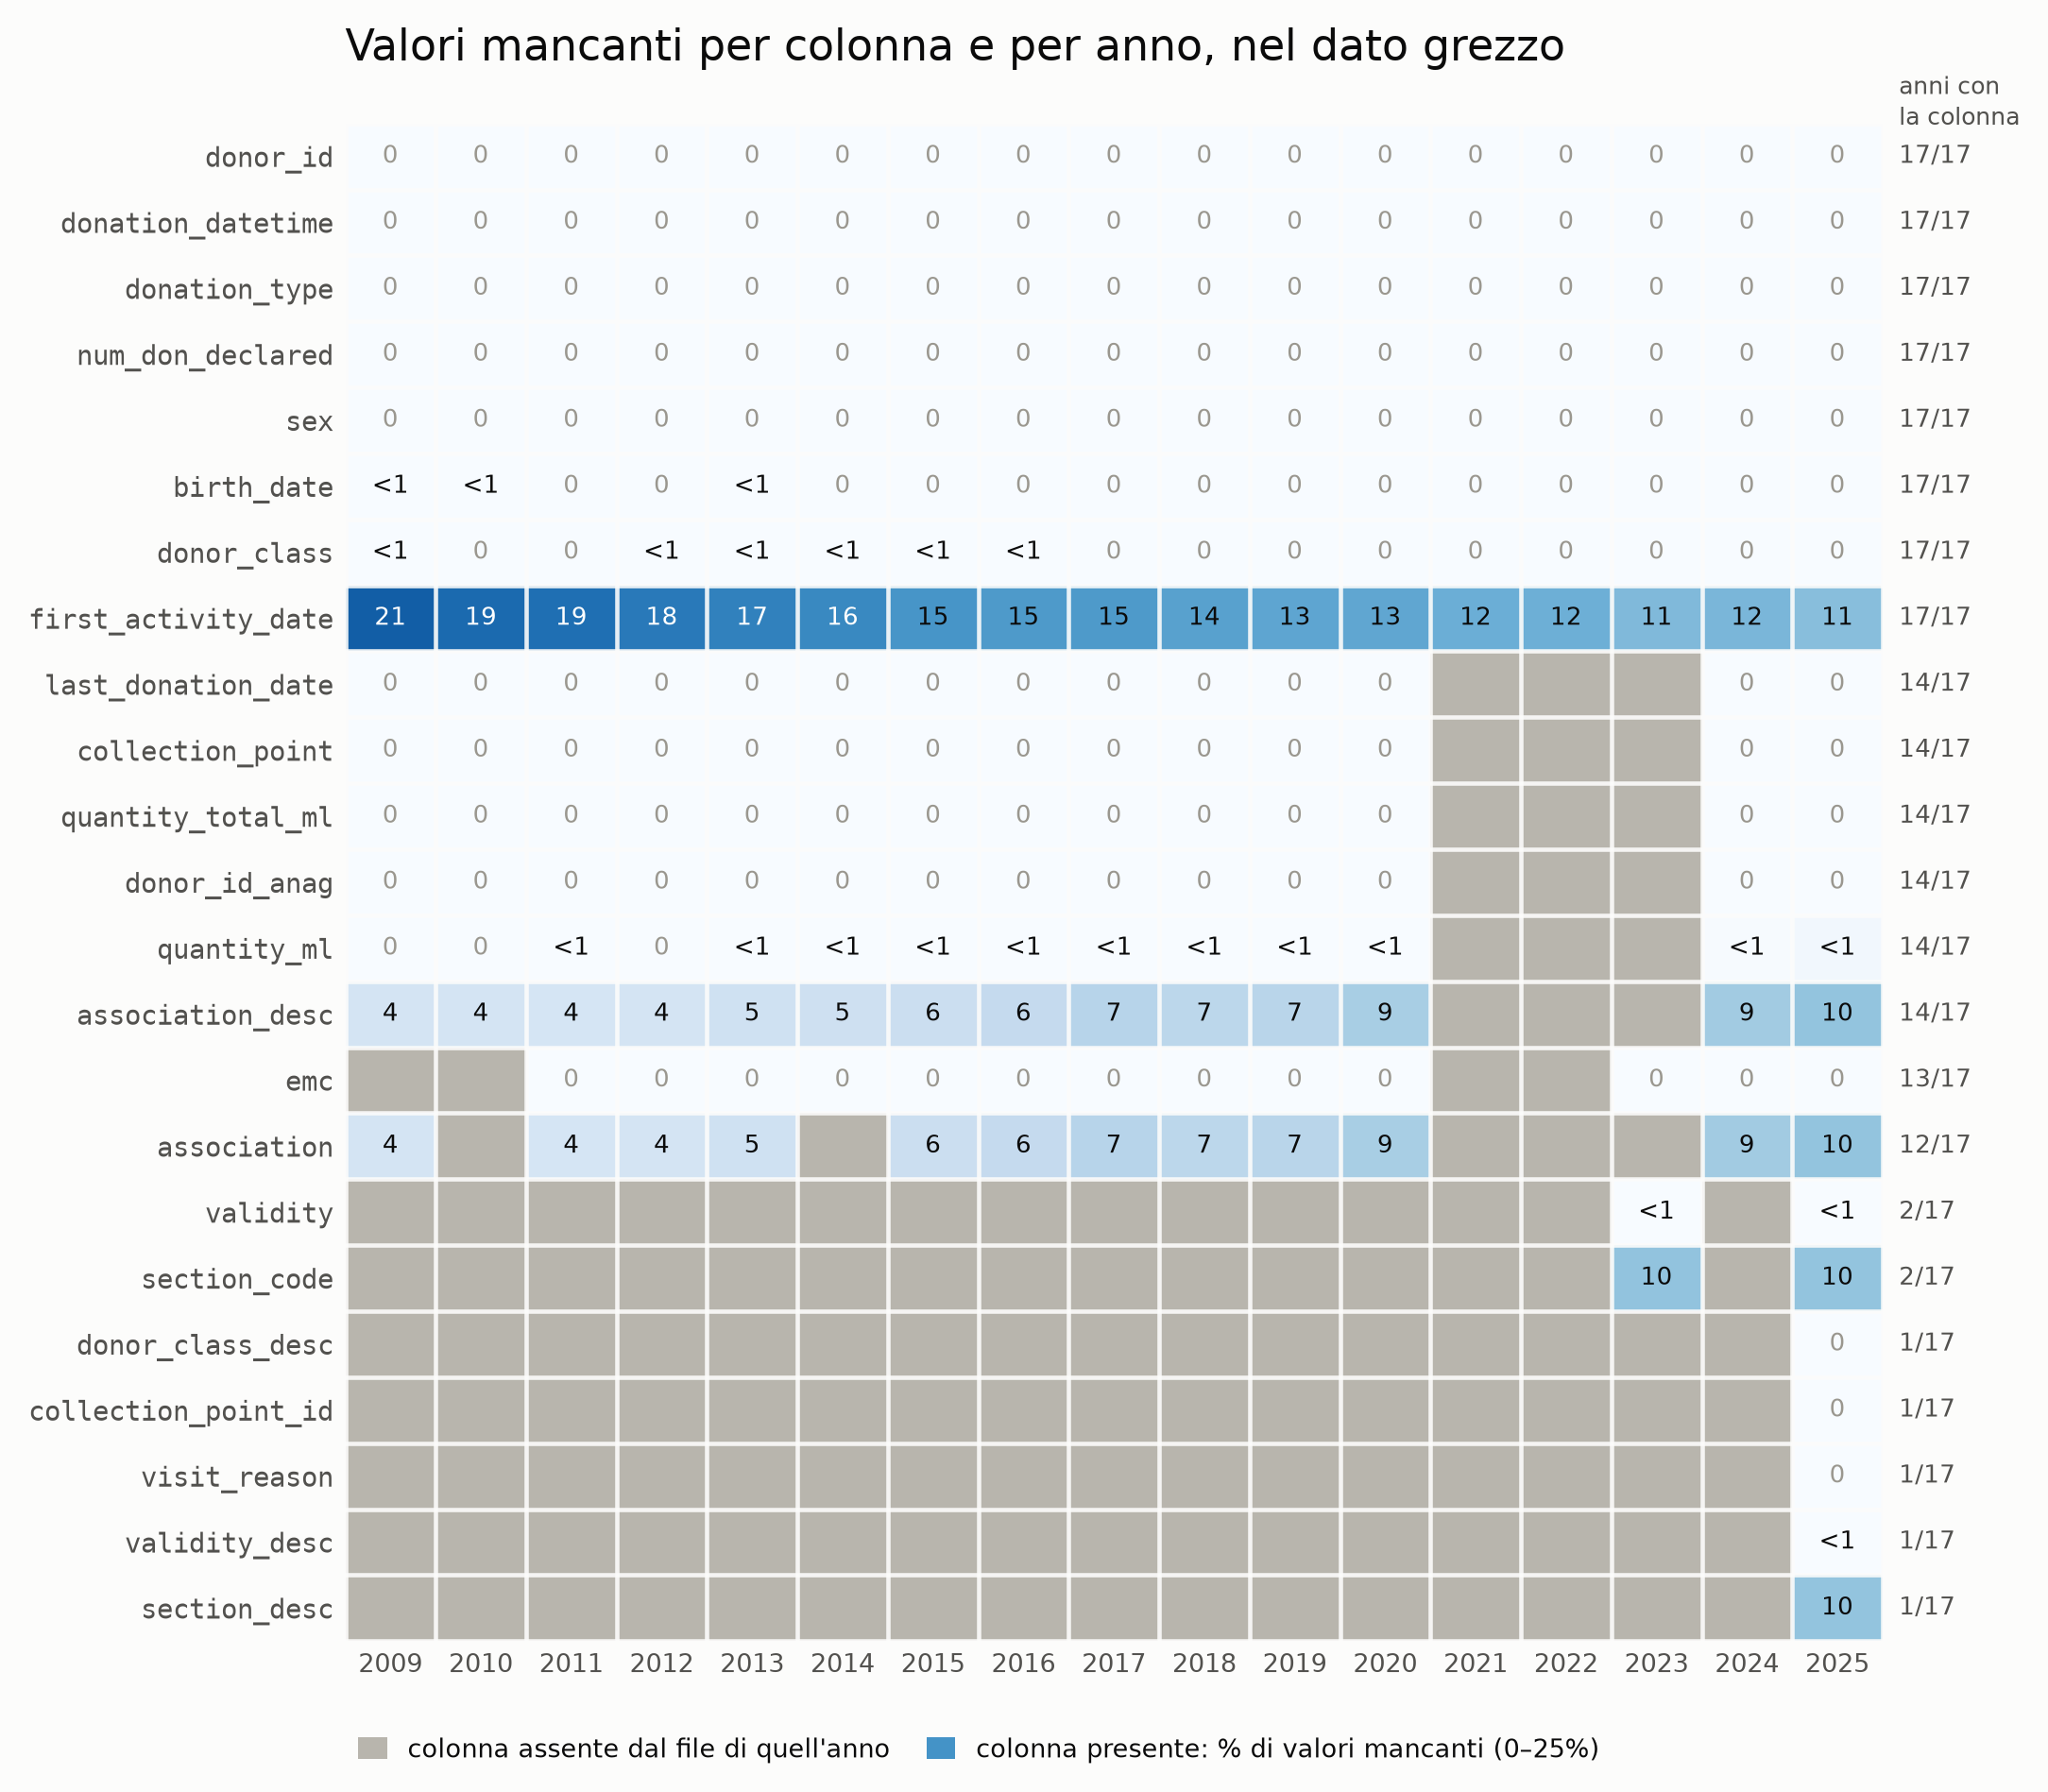
\includegraphics[width=0.95\linewidth]{img/fig_null_heatmap.png}
    \caption{Valori mancanti per colonna e per anno nei file sorgente, prima
    di qualsiasi elaborazione. Il grigio indica una colonna che in quell'anno
    non esiste affatto; dove la colonna esiste, il numero è la percentuale di
    valori mancanti e l'intensità del blu vi è proporzionale. Le due
    condizioni sono tenute separate perché dicono cose diverse: la prima è una
    proprietà del tracciato, la seconda del dato.}
    \label{fig:null_heatmap}
\end{figure}

% ───────────────────────────────────────────────────────────────────────
\section{Due decisioni che condizionano tutto il resto}
\label{sec:decisioni}

\paragraph{Quale colonna identifica il donatore.}
I file contengono due identificativi anonimi, \texttt{crd} e \texttt{id\_anag}.
Solo il primo è presente in \textbf{tutti e 27 i file}; il secondo manca nei
file 2021, 2022 e in entrambi i file 2023. La corrispondenza fra i due è di
fatto biunivoca: su 41\,201 valori distinti di \texttt{crd}, soltanto
\textbf{tre} sono associati a più di un \texttt{id\_anag}, e nessun
\texttt{id\_anag} è associato a più di un \texttt{crd}.

La scelta ricade quindi su \texttt{crd}:
adottare \texttt{id\_anag} costringe a ricostruire l'identità del donatore per
il triennio 2021--2023 con una mappatura di copertura parziale, e ogni donatore
non mappato risulta artificialmente nuovo in quegli anni --- con effetti
diretti sul conteggio dei nuovi ingressi del \cref{ch:eda} e sulle coorti del
\cref{ch:retention}. Con \texttt{crd} il problema non si pone.

\paragraph{L'inizio dell'attività da donatore è un importante predittore.}
La colonna \texttt{dtinizatt\_da} registra quando il soggetto ha cominciato a
donare, anche molto prima dell'inizio della finestra osservata. È \textbf{nulla
su 54\,017 righe}, e la sua compilazione dipende dalla prassi
della sede.

\begin{table}[ht]
\centering
\caption{Quota di righe prive di data di inizio attività, per punto di
raccolta. La compilazione è una prassi locale, non un attributo del donatore.}
\label{tab:nulli_sede}
\begin{tabular}{@{}lrr@{}}
\toprule
\textbf{Punto di raccolta} & \textbf{Righe} & \textbf{Senza data di inizio} \\
\midrule
Maggiore (Trieste)  & 152\,302 & \phantom{0}2{,}3\% \\
Burlo (Trieste)     & \phantom{0}12\,353 & \phantom{0}1{,}2\% \\
Autoemoteca TS      & \phantom{00}7\,091 & \phantom{0}0{,}3\% \\
Autoemoteca UD      & \phantom{00}3\,034 & 17{,}9\% \\
Autoemoteca GO      & \phantom{0}25\,475 & 23{,}0\% \\
Monfalcone S.\ Polo & \phantom{0}47\,601 & 29{,}2\% \\
Sede Gorizia        & \phantom{0}49\,727 & \textbf{45{,}7\%} \\
Cormons             & \phantom{000}533 & 49{,}2\% \\
Grado               & \phantom{00}1\,070 & 52{,}0\% \\
\midrule
Non registrato (2021--2023) & \phantom{0}54\,485 & 12{,}0\% \\
\bottomrule
\end{tabular}
\end{table}

A Trieste il campo è quasi sempre valorizzato, nell'Isontino spesso no
(\cref{tab:nulli_sede}). Ne segue che \textbf{scartare le righe prive di quel
campo equivale a cancellare in larga parte una provincia}: delle donazioni che
andrebbero perse, oltre tre quarti sono di Gorizia e Monfalcone. Il campo viene
quindi conservato come covariata, e dove manca resta mancante --- l'evento di
donazione, che è osservato senza ambiguità, non si butta. L'effetto sulla
geografia è discusso nella \cref{sec:collection}.

% ───────────────────────────────────────────────────────────────────────
\section{La pipeline}
\label{sec:cleaning}

La pipeline è organizzata in \textbf{quattro stadi} (\cref{fig:pipeline}). Ogni
stadio legge il file prodotto da quello precedente e ne scrive uno nuovo:
nessuno riscrive il proprio input, quindi ogni comando è rieseguibile senza
effetti d'ordine e una rielaborazione parziale non lascia il dataset in uno
stato intermedio.

\begin{figure}[H]
    \centering
    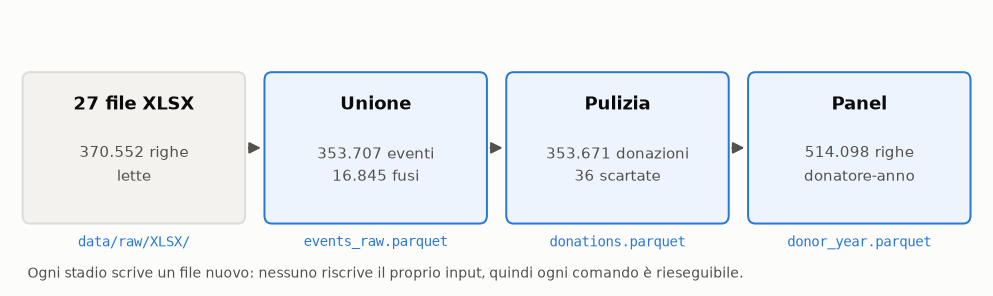
\includegraphics[width=\linewidth]{img/fig_pipeline_diagram.png}
    \caption{I quattro stadi della pipeline, con il numero di righe in uscita
    da ciascuno.}
    \label{fig:pipeline}
\end{figure}

\paragraph{Stadio 1 --- Unione.}
I 27 file vengono ricondotti allo schema comune e uniti. I due file 2023
meritano una nota: contengono \emph{lo stesso insieme di eventi} (16\,843 righe
ciascuno, chiavi coincidenti) e differiscono per una sola colonna,
\texttt{sez} nell'uno e \texttt{validita} nell'altro. Caricarli entrambi
raddoppierebbe l'anno; caricarne uno solo butterebbe via una colonna. Vengono
quindi \emph{fusi} sulla chiave dell'evento, conservando entrambe le colonne:
le 33\,686 righe dei due file si riducono a \textbf{16\,842 eventi} distinti.
La fusione è l'unica riduzione di questo stadio --- a essa si aggiunge una sola
riga, un duplicato interno al file 2024 --- per un totale di
\textbf{16\,845 righe} in meno, elencate una per una in un report di
riconciliazione.

\paragraph{Stadio 2 --- Pulizia.}
Ogni regola è una funzione separata che dichiara quante righe tocca. Le regole
applicate sono: normalizzazione delle date; filtro sull'età ammissibile
(18--90 anni, dove i valori oltre soglia sono errori evidenti di data di
nascita); consolidamento dei punti di raccolta, che nei file identificano il
singolo veicolo o turno e non la sede (\emph{Autoemoteca GO}, \emph{Seconda
autoemoteca GO}, \ldots) e vengono ricondotti a nove sedi; normalizzazione dei
codici di associazione, che si riducono a nove livelli.

Le tipologie di donazione minoritarie e le descrizioni di associazione
\emph{non} vengono invece accorpate in questo stadio: restano tutti i dieci
codici di tipologia e tutte le tredici descrizioni presenti nei file grezzi. Il
raggruppamento in una categoria residuale avviene, dove serve, a valle: nel
\cref{ch:glm} la tipologia prevalente pregressa usa una categoria
\textsc{altro} per i codici sotto soglia.

\paragraph{Stadio 3 --- Panel donatore-anno.}
L'ultimo stadio non pulisce: cambia unità di osservazione. Per ogni donatore si
costruisce una riga per \emph{ogni} anno dal suo ingresso in poi, anche per gli
anni in cui non ha donato. Gli anni a zero sono \textbf{il 63{,}9\%} delle
righe, e senza di essi l'abbandono --- l'evento che il \cref{ch:retention}
studia e che il \cref{ch:glm} vuole modellare --- semplicemente non
comparirebbe nei dati. La somma della risposta su un anno è, per costruzione,
il totale di quell'anno: aggregato e individuale non possono contraddirsi.

L'\cref{alg:panel} riassume la costruzione. Due dettagli non sono cosmetici. Il
primo è la riga~3: gli attributi del donatore si prendono alla \emph{prima}
riga osservata e non all'ultima, altrimenti in ogni anno del panel comparirebbe
informazione raccolta dopo. Il secondo è la riga~9, l'unica verifica che conta
davvero: se la somma della risposta non coincide con il numero di donazioni di
partenza, la costruzione si ferma.

\begin{algorithm}[H]
\caption{Costruzione del panel donatore-anno}
\label{alg:panel}
\begin{algorithmic}[1]
\Require eventi di donazione $D$; ultimo anno della finestra $T$
\Ensure panel $P$ con una riga per coppia (donatore, anno)
\State $A \gets$ conteggio di $D$ per (donatore, anno)
\Comment{solo gli anni in cui si è donato}
\State per ogni donatore $i$: attributi $x_i \gets$ valori della sua prima riga
osservata \Comment{mai dell'ultima: sarebbe informazione futura}
\State per ogni donatore $i$: $e_i \gets \min\{\,t : (i,t) \in A\,\}$
\Comment{anno d'ingresso}
\State $P \gets \{\,(i, t) : e_i \le t \le T\,\}$
\Comment{griglia densa: anche gli anni senza donazioni}
\State $y_{it} \gets A[i,t]$ se presente, altrimenti $0$
\Comment{è qui che nascono gli zeri}
\State $\text{carriera}_{it} \gets t - e_i$; \ \ $\text{età}_{it} \gets t -
\text{anno di nascita}_i$
\State unisci $x_i$ a ogni riga di $P$
\If{$\sum_{i,t} y_{it} \neq |D|$} \State \textbf{interrompi}
\Comment{il panel deve rendere conto di ogni donazione}
\EndIf
\State \Return $P$
\end{algorithmic}
\end{algorithm}

\begin{table}[H]
\centering
\small
\caption{Simboli dell'\cref{alg:panel} e valori sul dataset finale.}
\label{tab:panel_simboli}
\begin{tabularx}{\linewidth}{@{}l X l@{}}
\toprule
\textbf{Simbolo} & \textbf{Significato} & \textbf{Valore} \\
\midrule
$D$ & eventi di donazione del dataset pulito, uno per riga & --- \\
$|D|$ & numero di eventi & 353\,671 \\
$T$ & ultimo anno della finestra osservata & 2025 \\
$i$ & donatore & 43\,299 distinti \\
$t$ & anno solare & $e_i,\dots,T$ \\
$A$ & conteggi per (donatore, anno), solo per gli anni con almeno una donazione & --- \\
$A[i,t]$ & donazioni del donatore $i$ nell'anno $t$ & --- \\
$x_i$ & attributi fissi del donatore (genere, anno di nascita, \ldots), presi dalla prima riga osservata & --- \\
$e_i$ & anno d'ingresso: primo anno con una donazione & 2009--2025 \\
$P$ & panel: una riga per ogni coppia $(i,t)$ con $e_i \le t \le T$ & 514\,098 righe \\
$y_{it}$ & risposta: donazioni di $i$ nell'anno $t$, zero se non ha donato & 63{,}9\% di zeri \\
$\text{carriera}_{it}$ & anni trascorsi dall'ingresso, $t - e_i$ & $0,\dots,16$ \\
$\text{età}_{it}$ & età nell'anno $t$ & --- \\
\bottomrule
\end{tabularx}
\end{table}

\subsection{Bilancio quantitativo}
\label{sec:phaselog}

\begin{table}[ht]
\centering
\caption{Bilancio riga-per-riga della pipeline.}
\label{tab:cleaninglog}
\begin{tabular}{@{}llrr@{}}
\toprule
\textbf{Stadio} & \textbf{Operazione} & \textbf{Righe in uscita} & \textbf{Variazione} \\
\midrule
0 & Lettura dei 27 file          & 370\,552 & ---          \\
1 & Fusione degli eventi doppi   & 353\,707 & $-16\,845$   \\
2 & Regole di pulizia            & 353\,671 & $-36$        \\
3 & Panel donatore $\times$ anno & 514\,098 & (cambio di unità) \\
\bottomrule
\end{tabular}
\end{table}

Il bilancio \textbf{chiude a zero}: ogni riga letta o esce nel file finale o
compare, con la ragione, in uno dei due report di riconciliazione. Le regole di
pulizia scartano \textbf{36 righe su 370\,552}, meno di un decimillesimo: è la
conseguenza diretta della scelta della \cref{sec:decisioni} di non usare la
completezza di un campo amministrativo come criterio di ammissione.

% ───────────────────────────────────────────────────────────────────────
\section{Struttura del dataset finale}
\label{sec:dataset}

Il dataset di eventi contiene \textbf{353\,671 righe}, una per donazione,
relative a \textbf{43\,299 donatori distinti} nel periodo 2009--2025. La chiave
naturale è la tripla (\texttt{donor\_id}, \texttt{donation\_datetime},
\texttt{donation\_type}). Il panel derivato ne conta \textbf{514\,098}, una per
coppia donatore-anno.

\small
\setlength{\tabcolsep}{4pt}
\begin{longtable}{@{}llp{7.6cm}@{}}
\caption{Dizionario delle variabili del dataset di eventi.}
\label{tab:columns} \\
\toprule
\textbf{Colonna} & \textbf{Tipo} & \textbf{Descrizione} \\
\midrule
\endfirsthead
\multicolumn{3}{l}{\textit{(continua dalla pagina precedente)}} \\
\toprule
\textbf{Colonna} & \textbf{Tipo} & \textbf{Descrizione} \\
\midrule
\endhead
\midrule
\multicolumn{3}{r}{\textit{(continua nella pagina seguente)}} \\
\endfoot
\bottomrule
\endlastfoot
\texttt{donor\_id}             & stringa  & Identificativo anonimo (\texttt{crd}) \\
\texttt{donation\_datetime}    & datetime & Data e ora dell'evento \\
\texttt{donation\_year}        & int      & Anno dell'evento \\
\texttt{donation\_month}       & int      & Mese dell'evento (1--12) \\
\texttt{donation\_type}        & stringa  & Tipo (\textsc{sangue}, \textsc{plasmaf}, \ldots) \\
\texttt{sex}                   & stringa  & Sesso (M / F) \\
\texttt{birth\_date}           & data     & Data di nascita \\
\texttt{age}                   & int      & Età al momento della donazione \\
\texttt{donor\_class}          & stringa  & Classe donatore (P, O, D, A) \\
\texttt{donor\_class\_regime}  & stringa  & Regime di codifica della classe (\cref{sec:glm_effects}) \\
\texttt{association}           & stringa  & Codice associazione \\
\texttt{association\_desc}     & stringa  & Nome associazione \\
\texttt{collection\_point}     & stringa  & Sede di raccolta consolidata \\
\texttt{first\_activity\_date} & data     & Inizio dell'attività donazionale \\
\texttt{last\_donation\_date}  & data     & Ultima donazione registrata \\
\texttt{quantity\_ml}          & float    & Quantità donata nell'evento (mL) \\
\texttt{validity}              & stringa  & Validità dichiarata (in 4 file su 27) \\
\texttt{num\_don\_declared}    & int      & Conteggio dichiarato --- \emph{solo controllo} \\
\texttt{quantity\_total\_ml}   & float    & Quantità cumulativa --- \emph{solo controllo} \\
\texttt{donor\_id\_anag}       & stringa  & Identificativo alternativo --- \emph{solo controllo} \\
\end{longtable}

\paragraph{Due colonne non esplicative.}
\texttt{num\_don\_declared} e \texttt{quantity\_total\_ml} sono conservate
soltanto come controllo e non compaiono in nessun modello. La prima non è un
attributo dell'evento ma un aggregato di livello superiore --- il numero di
donazioni del gruppo (donatore, anno, tipologia) --- replicato su ciascuna riga
del gruppo; coincide con il conteggio osservabile nel $96{,}1\%$ dei casi. La
seconda è la somma delle quantità nello stesso gruppo, quindi è la risposta
moltiplicata per un volume medio. \textbf{Il conteggio delle donazioni si
ottiene sempre contando le righe.} Il punto è ripreso nella
\cref{sec:glm_unit}, dove ha conseguenze dirette sulla specifica del modello.

\paragraph{Donazioni dichiarate non valide.}
La colonna \texttt{validity} esiste solo in 4 file su 27 e marca 752 donazioni
come non valide. Non essendo applicabile in modo uniforme all'intero periodo,
non viene usata come filtro: quelle righe restano nel conteggio, e la variante
che le esclude è stata verificata come analisi di sensitività senza effetti
apprezzabili sui risultati dei capitoli seguenti.

% ───────────────────────────────────────────────────────────────────────
\section{Sintesi del capitolo}
\label{sec:datasummary}

Il dataset analitico finale contiene \textbf{353\,671 eventi di donazione}
relativi a \textbf{43\,299 donatori} osservati fra il 2009 e il 2025, ottenuti
da 27 file Excel attraverso quattro stadi, ciascuno dei quali produce un file
nuovo e un bilancio verificabile. La riduzione complessiva rispetto al dato
grezzo è di 16\,881 righe, quasi interamente dovuta alla fusione delle due
estrazioni del 2023.

Le due decisioni che pesano di più --- usare \texttt{crd} come identificativo e
trattare la data di inizio attività come covariata anziché come requisito ---
sono quelle che determinano quanto dato arriva alle analisi. La seconda in
particolare ha un effetto geografico: valutarla diversamente significa
raccontare l'Isontino con circa la metà delle sue donazioni.

% ══════════════════════════════════════════════════════════════════════════════
%  Fine Capitolo — Dati e Costruzione del Dataset
% ══════════════════════════════════════════════════════════════════════════════

% ══════════════════════════════════════════════════════════════════════════════
%  CAPITOLO — ANALISI ESPLORATIVA DEI DATI
%  Etichette: ch:eda, sec:demo, sec:types, sec:temporal, sec:collection,
%             sec:intensity, sec:denominatore, sec:eda_summary
% ══════════════════════════════════════════════════════════════════════════════

\chapter{Analisi Esplorativa dei Dati}
\label{ch:eda}

L'analisi che segue è basata sul dataset finale del \cref{ch:data}:
\textbf{353\,671 donazioni} di \textbf{43\,299 donatori distinti}, 2009--2025,
raccolte presso i punti di prelievo del DIMT di Trieste e Gorizia.

Il capitolo persegue tre scopi: descrivere chi sono i donatori; mostrare come e
dove donano; ed evidenziare le tendenze temporali che motivano la struttura dei
modelli dei capitoli successivi. La \cref{sec:denominatore} aggiunge una quarta
domanda, che le prime tre non possono rispondere: quanto del movimento
osservato è comportamento e quanto è semplicemente demografia.

% ---------------------------------------------------------------
\section{Profilo demografico dei donatori}
\label{sec:demo}

La popolazione di donatori è composta da \textbf{26\,737 uomini (61{,}7\%)} e
\textbf{16\,562 donne (38{,}3\%)}, con un rapporto M/F di circa $1{,}61$
(\cref{fig:gender}). La prevalenza maschile è sostanziale ed è in linea con i
dati nazionali del Centro Nazionale Sangue~\cite{cns2020}. La minore presenza femminile è
coerente con le restrizioni cliniche: prima della menopausa le donne possono
donare sangue intero due volte l'anno anziché quattro, e non possono donare
durante le mestruazioni o la gravidanza~\cite{donneDonazione}.

\begin{figure}[H]
    \centering
    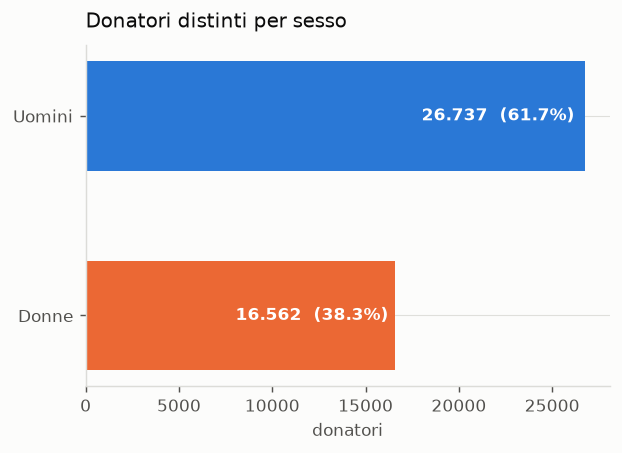
\includegraphics[width=0.55\linewidth]{img/fig_gender.png}
    \caption{Composizione per sesso dei donatori distinti, 2009--2025.}
    \label{fig:gender}
\end{figure}

L'età alla donazione (\cref{fig:age_hist}) ha media \textbf{42{,}4 anni},
mediana \textbf{44} e deviazione standard \textbf{12{,}0}, e va dai 18 anni
(minima età legale) ai 74; l'estremo superiore è coerente con la possibilità,
per i donatori periodici, di proseguire oltre i 65 anni sulla base della
valutazione clinica.

La forma non è però quella di una campana. Si riconoscono \textbf{due mode}:
un picco isolato a 18--19 anni --- l'effetto delle campagne di reclutamento
nelle scuole e della donazione al compimento della maggiore età --- seguito da
un avvallamento fra i 20 e i 30, e poi la moda principale intorno ai 47 anni,
su cui si concentra la massa della distribuzione. La fascia 30--55 rappresenta
la quota maggioritaria delle donazioni, mentre la 18--29 contribuisce con una
porzione minore --- un dato che la \cref{sec:denominatore} rileggerà, perché in
valore assoluto non dice quello che sembra dire.

\begin{figure}[H]
    \centering
    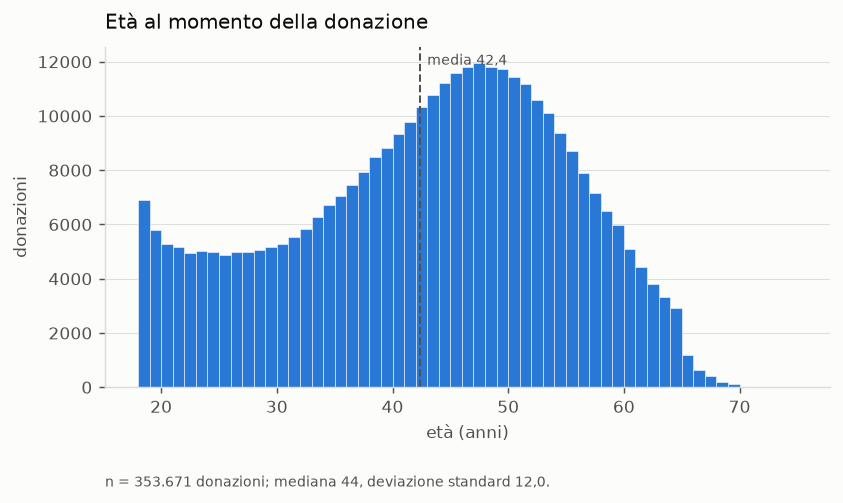
\includegraphics[width=0.85\linewidth]{img/fig_age_hist.png}
    \caption{Distribuzione dell'età al momento della donazione.}
    \label{fig:age_hist}
\end{figure}

Quanto all'adesione ad associazioni di volontariato (AVIS, ADSPEM, FIDAS e
altre), l'\textbf{81{,}7\%} dei donatori risulta associato in almeno una delle
proprie donazioni.

% ---------------------------------------------------------------
\section{Tipologie di donazione}
\label{sec:types}

Il dataset distingue dieci codici corrispondenti a sangue intero, plasmaferesi,
aferesi multicomponente e prelievi specialistici. Tre tipologie concentrano
il $99{,}7\%$ del volume (\cref{fig:types}): \textbf{sangue intero}
(267\,259 donazioni, $75{,}6\%$), \textbf{plasmaferesi} (75\,746, $21{,}4\%$) e
\textbf{aferesi piastrine + plasma} (9\,579, $2{,}7\%$). Le restanti sette
sommano circa lo $0{,}3\%$ (1\,087 donazioni) --- la più rara, la granulocitoaferesi, compare una
volta sola --- e nel dataset restano distinte; per semplicità, esse verranno accorpate in
un'unica categoria, "Altro", per le analisi successive.

\begin{figure}[H]
    \centering
    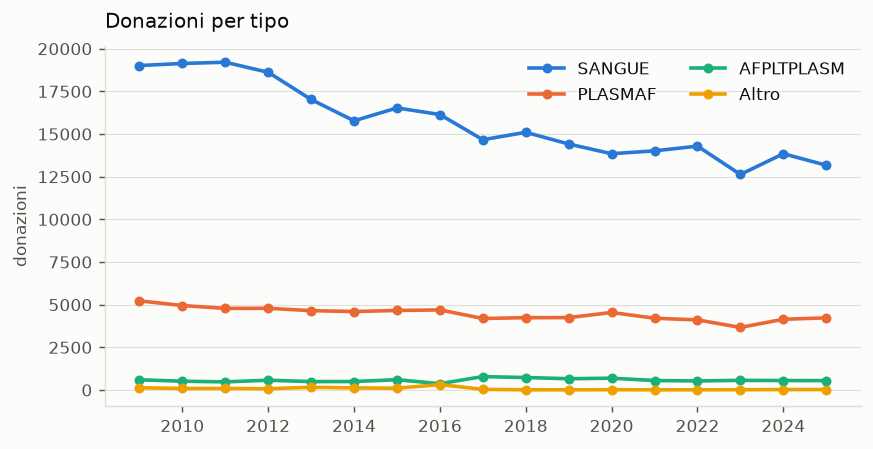
\includegraphics[width=0.80\linewidth]{img/fig_donation_types.png}
    \caption{Distribuzione delle donazioni per tipologia, 2009--2025.}
    \label{fig:types}
\end{figure}

\paragraph{Evoluzione della composizione nel tempo.}
La quota della plasmaferesi si mantiene sostanzialmente stabile
(\cref{fig:types_time}), con oscillazioni contenute in pochi punti percentuali
lungo tutto il periodo. La direzione è coerente con la spinta nazionale verso
l'autosufficienza~\cite{autosufficienza}, ma l'entità dell'effetto nel dataset
è modesta: la composizione per tipologia è la dimensione più immobile di tutto
il quadro descrittivo, e l'\cref{ch:forecast} la proietterà tale.

\begin{figure}[H]
    \centering
    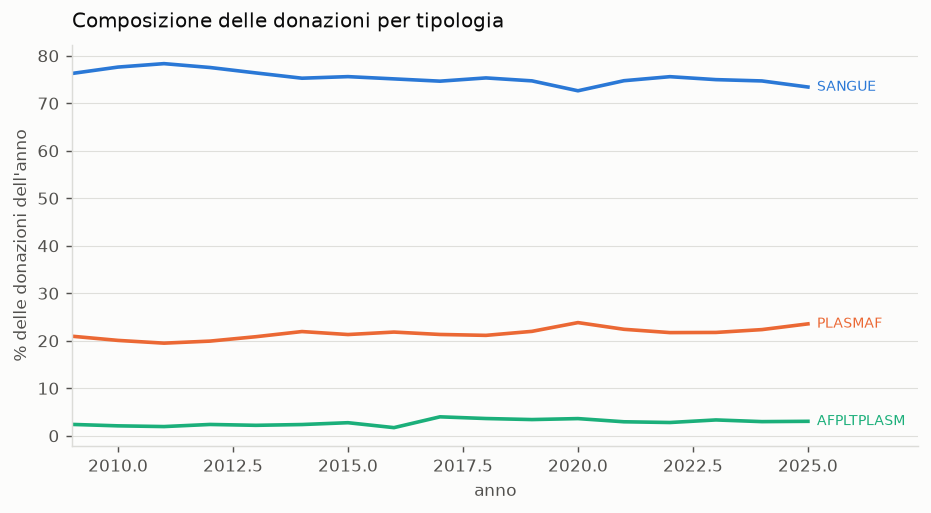
\includegraphics[width=0.95\linewidth]{img/fig_types_over_time.png}
    \caption{Composizione percentuale delle donazioni per tipologia, anno per
    anno.}
    \label{fig:types_time}
\end{figure}

% ---------------------------------------------------------------
\section{Tendenze temporali}
\label{sec:temporal}

\paragraph{Donazioni annuali.}
Il volume parte da circa \textbf{24\,900 donazioni} nel 2009, scende in modo
regolare fino a poco meno di 19\,300 nel 2019 e si assesta poi attorno alle
17--18 mila. Fra il primo e l'ultimo anno osservato la contrazione è del
\textbf{28{,}1\%} (\cref{fig:don_per_year}).

L'impatto della pandemia sul 2020 è stato \emph{più contenuto di quanto ci si
potesse attendere}: 19\,060 donazioni contro le 19\,289 del 2019, un calo
dell'$1{,}2\%$. Il dato è coerente con la posizione del Centro Nazionale
Sangue~\cite{cns2020} sulla tenuta del sistema trasfusionale italiano nei mesi
di lockdown, dovuta al
riconoscimento della donazione come attività essenziale e a un'ondata di
mobilitazione spontanea nelle prime settimane. Il 2023 segna il minimo della
serie (16\,840), con un parziale recupero nel biennio successivo.

\begin{figure}[H]
    \centering
    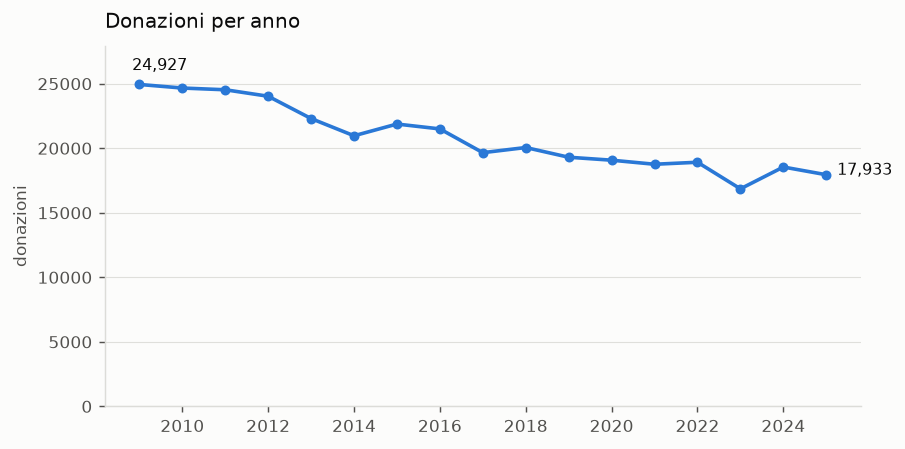
\includegraphics[width=0.95\linewidth]{img/fig_donations_per_year.png}
    \caption{Donazioni totali per anno, 2009--2025.}
    \label{fig:don_per_year}
\end{figure}

\paragraph{Nuovi donatori, e perché il 2009 non conta.}
Un secondo indicatore è il numero di donatori che entrano nel sistema ogni
anno. Qui però il primo anno della finestra non è un anno come gli altri: chi
compare per la prima volta nel 2009 non necessariamente \emph{inizia} nel 2009,
può semplicemente essere il primo anno in cui lo vediamo.

Il dato grezzo permette di distinguere i due casi, perché contiene la data di
inizio dell'attività donazionale (\cref{sec:decisioni}). Il risultato è netto:
dei 12\,957 donatori che nel 2009 risultano al primo evento osservato,
\textbf{il 65{,}9\% aveva già cominciato a donare prima}. Per loro la carriera
era iniziata, in mediana, nel 2002. Nel 2010 la quota di ``falsi ingressi'' è
ancora del $46{,}1\%$; dal 2011 in poi si stabilizza fra il 16 e il 29 per
cento, riflettendo il fatto che il campo non è sempre compilato.

L'avvio del sistema informativo nazionale SISTRA~\citep{sistra2007}, che le
Regioni dovevano recepire entro il 2008, spiega bene il fenomeno: donatori già
attivi da tempo ma non ancora tracciati elettronicamente compaiono come
``nuovi'' nel primo anno di rilevazione. La \cref{fig:new_donors} distingue le
due componenti; nel seguito \textbf{il 2009 è escluso dai confronti sui nuovi
ingressi}, e la flessione si misura dal 2010: da \textbf{1\,860 a 1\,149}
ingressi genuini fra il 2010 e il 2025, cioè $-38{,}2\%$, con un minimo di 960
nel 2021.

Qui è
considerato genuino chi non risulta \emph{esplicitamente} attivo prima, il che
include i donatori per cui la data di inizio manca del tutto: la domanda del
capitolo è quanti ingressi il sistema registra ogni anno, e togliere chi non ha
il campo compilato significherebbe togliere l'Isontino, per la ragione della
\cref{sec:decisioni}. Nel \cref{ch:retention}, in cui invece si segue una
coorte nel tempo, si adotta il criterio più restrittivo e si tiene solo chi ha una
data di inizio \emph{nota} e non anteriore all'anno del primo evento. Le due
serie divergono molto nei primi anni (nel 2010, 1\,860 contro 1\,360) e
convergono di fatto dal 2019 in poi, quando il campo è quasi sempre compilato.

\begin{figure}[H]
    \centering
    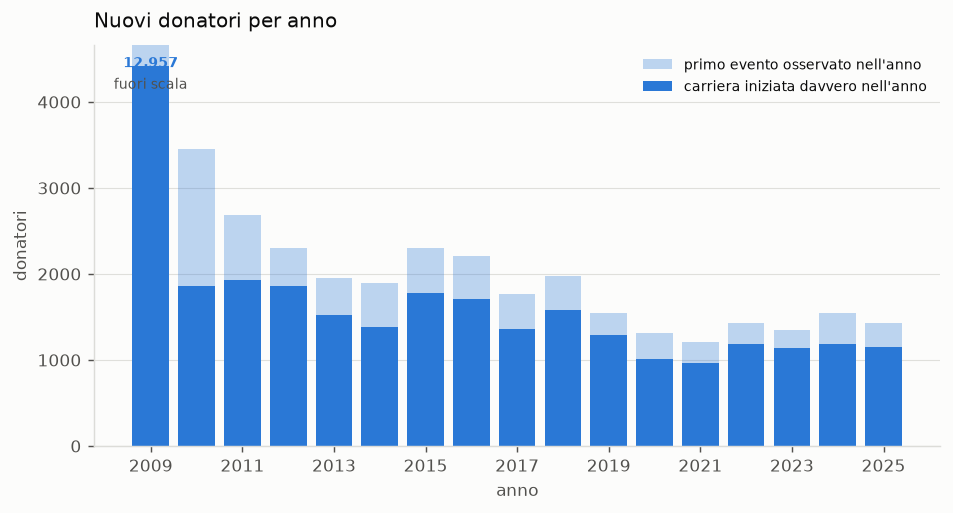
\includegraphics[width=0.95\linewidth]{img/fig_new_donors.png}
    \caption{Nuovi donatori per anno. La barra piena conta i soli donatori la
    cui attività comincia davvero in quell'anno; quella chiara aggiunge chi
    compare per la prima volta ma era già attivo prima.}
    \label{fig:new_donors}
\end{figure}

\paragraph{Stagionalità mensile.}
Sotto l'ipotesi di assenza di stagionalità ogni mese contribuirebbe all'$8{,}33\%$
del totale. Si osservano invece un picco primaverile (\textbf{marzo},
$9{,}24\%$) e autunnale (\textbf{ottobre}, $9{,}03\%$; settembre $8{,}80\%$),
un avvallamento estivo (\textbf{agosto}, $7{,}60\%$; luglio $7{,}86\%$) e uno
invernale meno marcato (\textbf{febbraio}, $7{,}95\%$), tipicamente associato
alle sospensioni per sindromi influenzali (\cref{fig:season}).

L'ampiezza è dell'ordine di $\pm 1$ punto percentuale: modesta ma sistematica.
Per evitare che il modello dell'\cref{ch:forecast} confonda questa variabilità
con il trend di lungo periodo, il mese vi entra come fattore esplicito.

\begin{figure}[H]
    \centering
    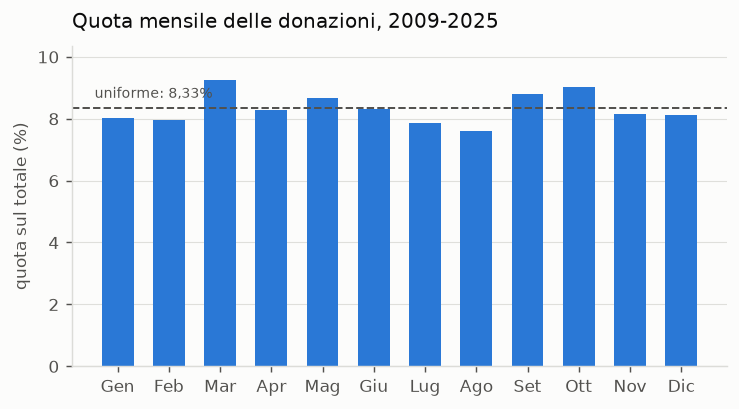
\includegraphics[width=0.95\linewidth]{img/fig_monthly_seasonality.png}
    \caption{Quota mensile delle donazioni sull'intero periodo. La linea
    tratteggiata indica la distribuzione uniforme attesa ($8{,}33\%$).}
    \label{fig:season}
\end{figure}

% ---------------------------------------------------------------
\section{Distribuzione geografica: punti di raccolta}
\label{sec:collection}

Il punto di raccolta non è registrato nei file del triennio 2021--2023, che hanno
un tracciato ridotto (\cref{sec:rawdata}): 54\,485 donazioni, il $15{,}4\%$ del
totale, ne sono prive, e le quote che seguono si riferiscono agli altri
quattordici anni. Sulle 299\,186 donazioni con punto di raccolta noto, l'ospedale
\textbf{Maggiore di Trieste} è di gran lunga il principale (152\,302
donazioni, $50{,}9\%$), seguito dalla \textbf{Sede di Gorizia} (49\,727,
$16{,}6\%$) e da \textbf{Monfalcone San Polo} (47\,601, $15{,}9\%$)
(\cref{fig:cp}).

Il dato ha una conseguenza sostanziale: \textbf{Gorizia non è un terzo polo
staccato, è appaiata a Monfalcone}, e i due siti isontini insieme valgono quasi
un terzo del sistema qui osservato. È l'effetto diretto della scelta discussa nella
\cref{sec:decisioni}: trattare la data di inizio attività come requisito di
ammissione avrebbe rimosso quasi la metà delle donazioni di Gorizia, che è
esattamente la sede in cui quel campo è meno compilato.

\begin{figure}[H]
    \centering
    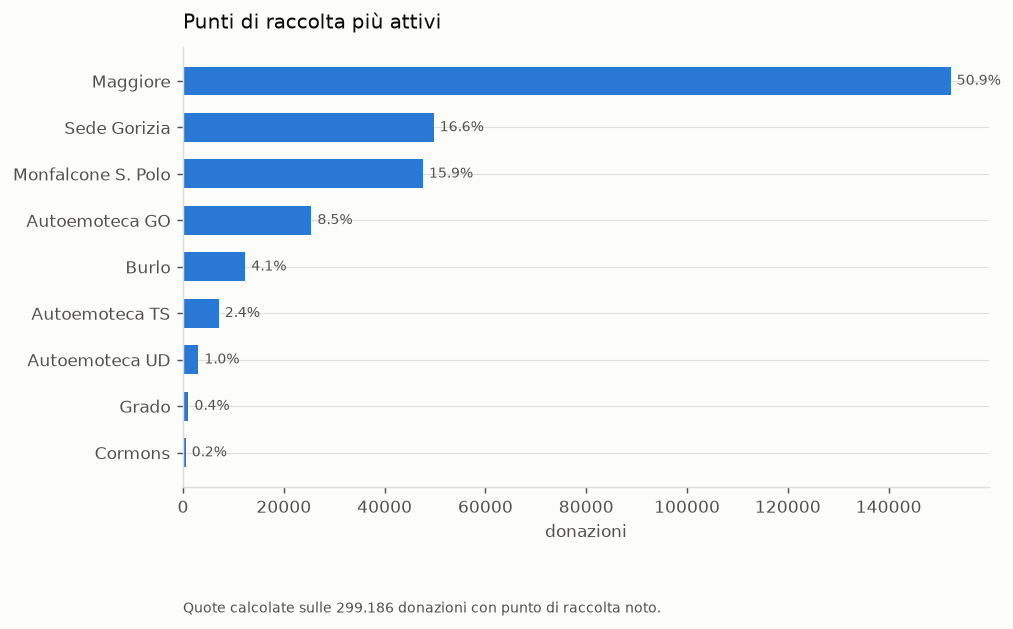
\includegraphics[width=0.95\linewidth]{img/fig_collection_points.png}
    \caption{Punti di raccolta più attivi, 2009--2025.}
    \label{fig:cp}
\end{figure}

% ---------------------------------------------------------------
\section{Intensità donazionale individuale}
\label{sec:intensity}

La distribuzione del numero di donazioni per donatore (\cref{fig:numdon}) è
fortemente asimmetrica a destra, con un notevole eccesso di donatori a una sola
donazione registrata e una coda lunga.

Va però osservato che questa figura misura la \emph{carriera}, non la
frequenza: somma donatori con due anni di attività e donatori con diciassette.
La misura pertinente per i modelli è il conteggio \emph{annuo}, sul panel
donatore-anno con gli anni a zero inclusi. Su quella misura la varianza è
$2{,}45$ volte la media: sovradispersione netta, che il \cref{ch:glm} dovrà
trattare esplicitamente. Sulla sola carriera dei donatori attivi il rapporto
scende a $1{,}23$, cioè quasi equidispersione --- lo stesso dato può quindi
sembrare o non sembrare sovradisperso a seconda dell'unità su cui lo si misura,
ed è una distinzione a cui il \cref{ch:glm} torna.

\begin{figure}[H]
    \centering
    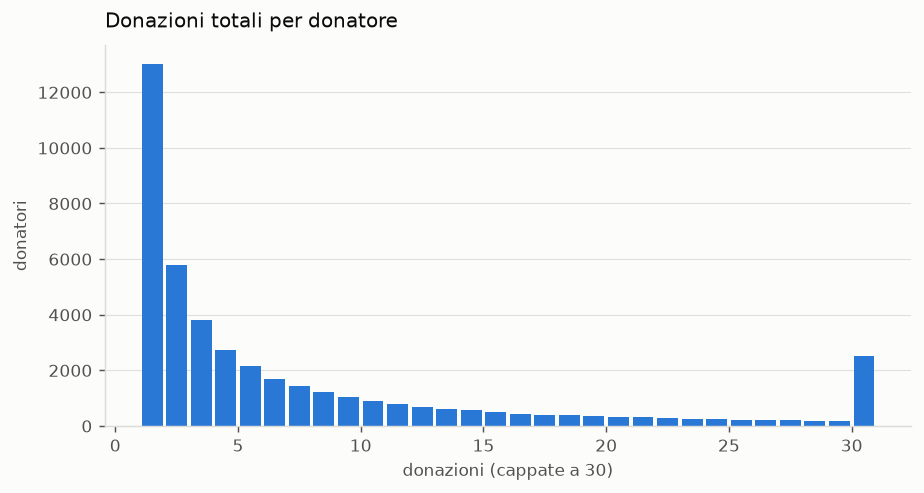
\includegraphics[width=0.85\linewidth]{img/fig_num_donations.png}
    \caption{Distribuzione del numero totale di donazioni per donatore (valori
    cappati a 30 per leggibilità).}
    \label{fig:numdon}
\end{figure}

Una seconda misura, meno vistosa ma più informativa, è il numero medio di
donazioni per donatore attivo in un anno. Resta in una banda di
\textbf{1{,}84--1{,}97 per tutti e diciassette gli anni}, senza tendenza: i
donatori attivi non donano oggi né più né meno spesso di quanto facessero nel
2009.

% ---------------------------------------------------------------
\section{Un denominatore: la popolazione residente}
\label{sec:denominatore}

Tutte le misure viste finora sono conteggi assoluti. Ma il territorio da cui
proviene il dato --- le province di Trieste e Gorizia --- perde abitanti e
invecchia: una parte del calo delle donazioni è meccanica, e finché non si
separano le due componenti l'affermazione ``il sistema è in erosione'' resta
indecidibile. La verifica è diretta: basta dividere per la popolazione in età
donabile.

\textbf{Il denominatore: popolazione di Trieste e Gorizia, non dell'intera
regione.} I dati di popolazione usati qui provengono da Eurostat al livello
NUTS-3 (\texttt{demo\_r\_pjanaggr3}, geo \texttt{ITH43} = Gorizia e
\texttt{ITH44} = Trieste~\cite{eurostatPjanaggr3NUTS3}), sommate fra le due
province: è la stessa area coperta dal DIMT e dalle donazioni al numeratore.
A questo livello di dettaglio geografico Eurostat pubblica solo tre fasce
ampie (\emph{under 15}, \emph{15--64}, \emph{65 e oltre}), non le fasce
quinquennali disponibili a livello regionale: si usa quindi la fascia
15--64 come proxy della popolazione in età donabile (18--64), leggermente più
ampia di quella esatta, perché le classi 15--17 pesano poco sul totale.

\paragraph{Quasi tutto il calo non è demografia.}
La popolazione di Trieste e Gorizia di 15--64 anni passa da 233\,144 a
223\,959 abitanti fra il 2009 e il 2025 ($-3{,}9\%$). Poiché le donazioni
sono il prodotto di quante persone potrebbero donare per quanto spesso lo
fanno, in logaritmi la variazione totale è la somma esatta delle due
componenti, senza residuo (\cref{tab:decomposizione}).

\begin{table}[ht]
\centering
\caption{Scomposizione del calo delle donazioni fra il 2009 e il 2025.}
\label{tab:decomposizione}
\begin{tabular}{@{}lrr@{}}
\toprule
\textbf{Componente} & \textbf{Variazione} & \textbf{Quota del calo} \\
\midrule
\textbf{Donazioni}                          & $-28{,}1\%$ & $100\%$ \\
\quad di cui: popolazione 15--64 (TS+GO)    & $\phantom{0}-3{,}9\%$  & $12{,}2\%$ \\
\quad di cui: donazioni per 1.000 residenti & $-25{,}1\%$ & $\mathbf{87{,}8\%}$ \\
\bottomrule
\end{tabular}
\end{table}

La demografia spiega poco meno di un \textbf{ottavo} del calo ($12{,}2\%$).
Quasi tutto il resto è perdita di partecipazione vera: si passa da
\textbf{106{,}9 a 80{,}1 donazioni ogni mille residenti} di 15--64 anni
(\cref{fig:per_1000}). Per il lavoro è un risultato che rafforza: l'erosione
è reale e non è un artefatto demografico. Senza il denominatore, l'obiezione
opposta sarebbe legittima e senza risposta.

\begin{figure}[H]
    \centering
    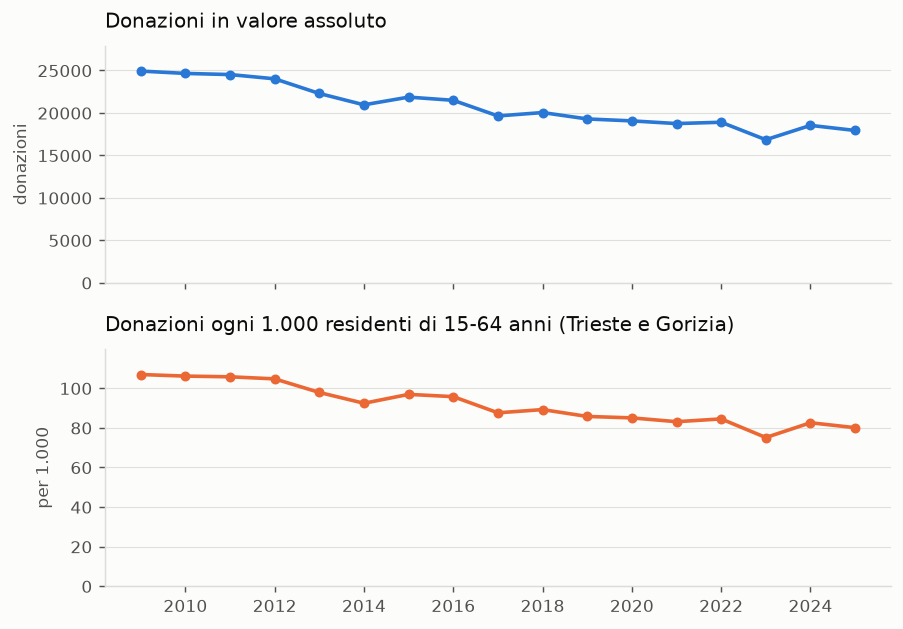
\includegraphics[width=0.9\linewidth]{img/fig_donazioni_per_1000.png}
    \caption{Donazioni in valore assoluto (sopra) e ogni mille residenti di
    15--64 anni di Trieste e Gorizia (sotto).}
    \label{fig:per_1000}
\end{figure}

\paragraph{Dove si è perso: non fra i giovani.}
Rapportando i donatori distinti alla popolazione della loro stessa fascia
d'età si ottiene il quadro della \cref{tab:tassi_eta}. Qui il denominatore
resta un limite dichiarato: a livello NUTS-3 Eurostat non pubblica fasce
quinquennali (\cref{sec:denominatore}), quindi questa tabella usa la
popolazione dell'intero Friuli Venezia Giulia
(\texttt{demo\_r\_pjangroup}~\cite{eurostatPjangroupNUTS2}) come proxy della
\emph{forma} del profilo per età, non del suo livello a Trieste e Gorizia. Il
quadro che ne risulta resta comunque controintuitivo rispetto a come la
questione viene di solito posta.

\begin{table}[ht]
\centering
\caption{Donatori distinti ogni mille residenti della stessa fascia d'età. Il
denominatore è la popolazione dell'intero Friuli Venezia Giulia (proxy della
forma del profilo, non del suo livello a Trieste e Gorizia).}
\label{tab:tassi_eta}
\begin{tabular}{@{}lrrr@{}}
\toprule
\textbf{Fascia} & \textbf{2009} & \textbf{2025} & \textbf{Variazione} \\
\midrule
\textbf{20--24} & $23{,}18$ & $\mathbf{19{,}21}$ & $-17{,}1\%$ \\
25--29 & $17{,}21$ & $17{,}64$ & $+2{,}5\%$ \\
30--34 & $18{,}75$ & $15{,}04$ & $-19{,}8\%$ \\
\textbf{35--39} & $21{,}14$ & $13{,}54$ & $\mathbf{-36{,}0\%}$ \\
\textbf{40--44} & $20{,}98$ & $12{,}37$ & $\mathbf{-41{,}0\%}$ \\
45--49 & $20{,}31$ & $14{,}72$ & $-27{,}5\%$ \\
50--54 & $16{,}58$ & $14{,}95$ & $\phantom{0}-9{,}8\%$ \\
55--59 & $12{,}21$ & $12{,}20$ & $\phantom{0}-0{,}1\%$ \\
60--64 & $\phantom{0}8{,}47$ & $\phantom{0}8{,}18$ & $\phantom{0}-3{,}4\%$ \\
65--69 & $\phantom{0}0{,}68$ & $\phantom{0}1{,}59$ & $+133{,}8\%$ \\
\bottomrule
\end{tabular}
\end{table}

Due letture, entrambe rilevanti per i capitoli successivi.

\textbf{Primo: a parità di popolazione, i giovani sono la fascia che dona di
più.} I 20--24enni hanno il tasso di partecipazione più alto in \emph{ogni}
anno osservato, 2025 compreso. Questo precisa i risultati ottenuti
nel \cref{ch:retention}: il problema dei giovani è che non
tornano a donare dopo le prime partecipazioni.

\textbf{Secondo: il crollo è a metà carriera.} Le fasce 35--44 perdono il
36--41\% del tasso di partecipazione, di gran lunga il calo maggiore, mentre le
fasce 55--64 sono sostanzialmente ferme e la 65--69 cresce (effetto
dell'estensione fino a 70 anni per i periodici). La \cref{fig:tassi_eta} lo
mostra in un colpo d'occhio: nel 2009 il profilo per età ha un ampio altopiano
fra i 35 e i 49 anni, nel 2025 quell'altopiano si è ristretto a un breve
pareggio fra i 45 e i 54 anni, e la curva scende in modo pressoché monotono
per tutte le fasce più giovani.

\begin{figure}[H]
    \centering
    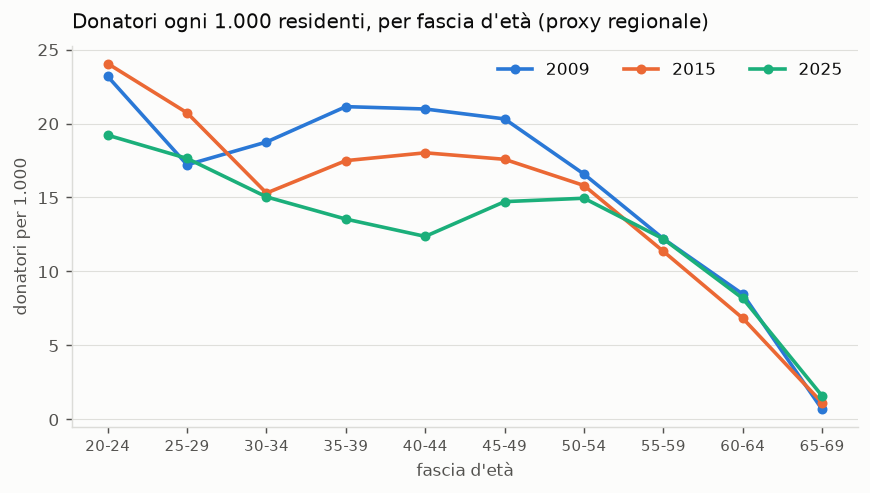
\includegraphics[width=0.9\linewidth]{img/fig_tassi_per_eta.png}
    \caption{Donatori ogni mille residenti per fascia d'età, in tre anni della
    serie.}
    \label{fig:tassi_eta}
\end{figure}

Il sistema, praticamente, ha perso i donatori di mezza età.
 Se questo sia un effetto di età o di coorte --- se cioè le
generazioni oggi trentacinquenni abbiano semplicemente sempre donato meno --- è
una domanda che i dati permettono di porre ma non, in questo lavoro, di
chiudere.

% ---------------------------------------------------------------
\section{Sintesi}
\label{sec:eda_summary}

\begin{enumerate}
    \item La popolazione di donatori è prevalentemente maschile ($61{,}7\%$) e
    di età media 42 anni: sesso ed età vanno controllati in tutti i modelli di
    frequenza.
    \item Il $99{,}7\%$ delle donazioni si concentra in tre tipologie, e la
    composizione fra queste è la dimensione più stabile del quadro.
    \item \textbf{Il volume annuale cala del $28{,}1\%$ fra il 2009 e il 2025},
    concentrando la flessione nella prima metà del periodo; i nuovi ingressi
    calano di più; e \textbf{l'intensità individuale non cambia}, restando fra
    $1{,}84$ e $1{,}97$ donazioni per donatore attivo. Il sistema non si è
    intensificato per compensare: si è ridotto e poi assestato su una base più
    piccola.
    \item \textbf{Solo un ottavo del calo è demografia} ($12{,}2\%$, sulla
    popolazione di Trieste e Gorizia), e la perdita di partecipazione si
    concentra nelle fasce 35--44, non fra i giovani, che restano la fascia
    con il tasso più alto. Resta un limite dichiarato sulla sola
    scomposizione \emph{per fascia d'età} (\cref{tab:tassi_eta}), che usa
    ancora la popolazione dell'intero FVG come proxy della forma del
    profilo, non essendo le fasce quinquennali disponibili a livello
    provinciale (\cref{sec:denominatore}).
    \item L'impatto del COVID-19 sul 2020 è stato modesto sulle donazioni
    ($-1{,}2\%$) ma marcato sui nuovi ingressi ($-21{,}5\%$): il modello aggregato
    deve poter assorbire uno shock puntuale.
    \item La stagionalità mensile è dell'ordine di $\pm 1$ punto percentuale,
    sistematica ma contenuta: va modellata come fattore per evitare confounding
    con il trend.
    \item La sovradispersione del conteggio dipende dall'unità di analisi:
    $2{,}45$ al grano donatore-anno con gli zeri, $1{,}23$ sui soli anni
    attivi. La scelta dell'unità nel \cref{ch:glm} non è quindi neutrale.
\end{enumerate}

% ══════════════════════════════════════════════════════════════════════════════
%  CAPITOLO — FIDELIZZAZIONE DEI DONATORI GIOVANI
%  Etichette: ch:retention, sec:ret_def, sec:ret_ident, sec:ret_dist,
%             sec:ret_survival, sec:ret_gender, sec:ret_comparison,
%             sec:ret_summary
% ══════════════════════════════════════════════════════════════════════════════

\chapter{Fidelizzazione dei Donatori Giovani}
\label{ch:retention}

La tenuta del sistema trasfusionale dipende non solo dal reclutare donatori ma
soprattutto dal \emph{trattenerli}. Il \cref{ch:eda} ha mostrato che gli
ingressi calano e che l'intensità individuale non compensa: resta da capire
quanto rapidamente si perde chi entra. La fascia d'ingresso \textbf{18--25
anni} ha un interesse particolare, perché chi inizia da giovane ha davanti il
massimo orizzonte di attività e, se fidelizzato, contribuisce per decenni; ed è
anche la fascia in cui l'abbandono dopo la prima donazione è tipicamente più
alto, per la mobilità geografica legata a studio e lavoro e per la minore
radicazione nelle reti associative.

Il capitolo misura quanti donatori giovani tornano, per quanti anni restano
attivi, se ci sono differenze fra maschi e femmine e come si collocano rispetto
a chi inizia in età più matura. Prima di tutto questo, però, va risolto un
problema di definizione che condiziona ogni numero del capitolo.

% ───────────────────────────────────────────────────────────────────────
\section{Chi è una coorte di ingresso}
\label{sec:ret_def}

Si definisce \textbf{donatore giovane} chi effettua la prima donazione fra i 18
e i 25 anni compiuti. La soglia inferiore è il limite legale in Italia; quella
superiore include l'intera finestra di transizione scuola--lavoro, ed è
coerente con la letteratura internazionale sulla donazione
giovanile~\cite{Maghsudlu2017}.

Il punto delicato è cosa si intende per \emph{prima} donazione. La finestra
osservata comincia nel 2009, ma il sistema trasfusionale no: come anticipato
nella \cref{sec:temporal}, dove due terzi dei ``nuovi'' del 2009 risultano già
attivi, il $30{,}4\%$ dei donatori presenti nel dataset aveva già cominciato a
donare prima del 2009. Per costoro la prima donazione
\emph{osservata} non è la prima donazione, e il primo anno in cui compaiono non
è il loro anno di ingresso.

L'errore non è innocuo, perché non è distribuito a caso: chi viene intercettato
a metà carriera è, per costruzione, un donatore che è già sopravvissuto alla
selezione per abbandono precoce, e quindi sopravvive più a lungo di una recluta
vera. Includerlo in una coorte di ingresso gonfia sistematicamente la curva di
sopravvivenza di quella coorte. Il problema è massimo proprio nella coorte
2009.

\begin{table}[ht]
\centering
\caption{Quota di ciascuna coorte apparente costituita in realtà da donatori
già attivi prima del loro primo anno osservato.}
\label{tab:coorti_composizione}
\begin{tabular}{@{}rrr@{\qquad}rrr@{}}
\toprule
\textbf{Coorte} & \textbf{Donatori} & \textbf{Già attivi} &
\textbf{Coorte} & \textbf{Donatori} & \textbf{Già attivi} \\
\midrule
\textbf{2009} & 1\,970 & \textbf{50{,}5\%} & 2016 & 943 & 12{,}7\% \\
2010 & \phantom{0}908 & 28{,}9\% & 2017 & 743 & 13{,}7\% \\
2011 & 1\,000 & 14{,}1\% & 2018 & 996 & 10{,}4\% \\
2012 & \phantom{0}972 & \phantom{0}8{,}2\% & 2019 & 764 & 10{,}7\% \\
2013 & \phantom{0}791 & 10{,}4\% & 2020 & 520 & 18{,}7\% \\
2014 & \phantom{0}810 & 13{,}8\% & 2021 & 566 & 14{,}5\% \\
2015 & \phantom{0}980 & 12{,}4\% & 2022 & 694 & 10{,}5\% \\
     &                &          & 2023 & 755 & \phantom{0}9{,}5\% \\
\bottomrule
\end{tabular}
\end{table}

La \cref{tab:coorti_composizione} rende la scala del problema: la coorte 2009 è
per \textbf{metà} composta da donatori già attivi, quella 2010 per oltre un
quarto, e dal 2011 in poi la quota oscilla fra l'8 e il 19 per cento, in
genere fra il 10 e il 14.
Ed è proprio la coorte 2009 quella che verrebbe naturale usare come esempio
principale delle curve di sopravvivenza, perché è la più numerosa e la più
lunga: è la coorte su cui l'errore pesa di più.

\paragraph{La correzione adottata.}
Nel seguito la coorte di ingresso comprende \textbf{soltanto i donatori la cui
attività comincia davvero dentro la finestra osservata}, cioè quelli per cui la
data di inizio attività è nota e cade nell'anno del primo evento registrato.
Escono dal calcolo due gruppi: i troncati a sinistra, che non appartengono in
senso proprio ad alcuna coorte osservabile, e --- necessariamente --- quelli
per cui la data di inizio \emph{manca}, di cui non si può dire se siano
reclute o veterani. Il secondo gruppo è la ragione per cui i conteggi di questo
capitolo non si ottengono sottraendo le quote della
\cref{tab:coorti_composizione} dai totali: la coorte 2009, ad esempio, conta
1\,970 donatori apparenti, di cui 994 già attivi prima e 185 senza data, e ne
restano 791 genuini. È anche il motivo per cui la serie di ingressi del
\cref{ch:eda}, che adotta il criterio più permissivo, è più alta di questa.

Va scartata invece una correzione che verrebbe naturale --- usare la data di
inizio attività come anno di ingresso e ricalcolare la retention da lì. Per chi
ha cominciato nel 2004 ed è osservato dal 2009 quel calcolo conterebbe cinque
anni di attività che nel dataset non ci sono, e produrrebbe una retention
\emph{più alta} di quella osservabile per una ragione puramente contabile. Le
due definizioni effettivamente adottate --- prima donazione osservata e solo
ingressi genuini --- sono calcolate entrambe per ogni misura del capitolo; 
nel testo si usa la seconda.

% ───────────────────────────────────────────────────────────────────────
\section{Consistenza del gruppo}
\label{sec:ret_ident}

Restringendo alle coorti 2009--2023 e osservando fino al 2025 --- così che
ogni coorte abbia almeno due anni di osservazione successiva --- il dataset
contiene \textbf{21\,085 ingressi genuini}. Di questi, \textbf{10\,552} sono
avvenuti fra i 18 e i 25 anni: \textbf{il 50{,}0\%} degli ingressi. I donatori
giovani così definiti generano \textbf{44\,237 donazioni} nel periodo osservato.

Il dato merita una sottolineatura, perché ribalta un'impressione: guardando
tutti i donatori presenti nel dataset i giovani sono un terzo, ma guardando
\emph{chi entra} sono la metà. Combinato con il risultato della
\cref{sec:denominatore} --- a parità di popolazione i 20--24enni sono la fascia
che dona di più --- il quadro è che il reclutamento giovanile funziona. È dopo
che si perde.

% ───────────────────────────────────────────────────────────────────────
\section{Distribuzione della retention}
\label{sec:ret_dist}

Per ogni donatore giovane si calcola la \textbf{retention}
$r = \text{ultimo anno} - \text{primo anno}$, cioè la distanza in anni fra
l'anno della prima e quello dell'ultima donazione osservata
(\cref{tab:ret_dist}). La misura è per anni solari: $r = 0$ indica chi dona in
un solo anno e non torna negli anni successivi, anche se in quell'anno ha
donato più di una volta.

\begin{table}[ht]
\centering
\caption{Distribuzione della retention per i 10\,552 donatori giovani entrati
fra il 2009 e il 2023, osservati fino al 2025.}
\label{tab:ret_dist}
\begin{tabular}{@{}rrrr@{}}
\toprule
\textbf{Anni di retention} & \textbf{Donatori} & \textbf{\%} & \textbf{\% cumulata} \\
\midrule
0  (un solo anno)      & 4\,281 & 40{,}6 & 40{,}6 \\
1                      & 1\,238 & 11{,}7 & 52{,}3 \\
2                      & \phantom{0}906 & \phantom{0}8{,}6 & 60{,}9 \\
3                      & \phantom{0}700 & \phantom{0}6{,}6 & 67{,}5 \\
4                      & \phantom{0}590 & \phantom{0}5{,}6 & 73{,}1 \\
5--9                   & 1\,819 & 17{,}2 & 90{,}4 \\
10+                    & 1\,018 & \phantom{0}9{,}6 & 100{,}0 \\
\midrule
\textbf{Totale}        & \textbf{10\,552} & \textbf{100{,}0} & \\
\bottomrule
\end{tabular}
\end{table}

Il risultato principale è la quota di donatori \textbf{``mordi e fuggi''}
($r = 0$): \textbf{il 40{,}6\%}. Due donatori giovani su cinque non tornano
negli anni successivi al primo (il $37{,}2\%$ dona una volta sola in assoluto).
Aggiungendo chi torna per un solo anno si arriva al \textbf{52{,}3\%}, che non
dona più dopo il secondo anno. All'altro estremo, il $26{,}9\%$ resta attivo
cinque anni o più e il $9{,}6\%$ almeno dieci --- un nucleo consolidato che
costituisce la componente strutturale del sistema.

Il numero mediano di donazioni per donatore giovane è \textbf{2} (media
$4{,}19$, deviazione standard $5{,}72$), con una coda che arriva a 122 donazioni
per il più assiduo: la stessa asimmetria della \cref{sec:intensity}.

% ───────────────────────────────────────────────────────────────────────
\section{Curve di sopravvivenza per coorte}
\label{sec:ret_survival}

Data la coorte entrata nell'anno $c$, si calcola la proporzione ancora attiva
nell'anno $c+k$. L'analisi è limitata alle coorti 2009--2018, per garantire un
orizzonte osservativo di almeno cinque anni.

La \cref{fig:ret_young} mostra a destra il confronto che vale la pena fare: la
coorte 2009 sotto le due definizioni, contro la banda di tutte le altre coorti.
Contando come coorte tutti i donatori al primo evento osservato, quella coorte
appare \emph{sopra} ogni altra a tutti gli orizzonti; sui soli ingressi
genuini rientra esattamente nella banda. Non era una
coorte più fedele: era mezza coorte di veterani.

\begin{table}[ht]
\centering
\caption{Sopravvivenza della coorte 2009 di donatori giovani, sotto le due
definizioni.}
\label{tab:ret_2009}
\begin{tabular}{@{}lrrrr@{}}
\toprule
& \textbf{1° anno} & \textbf{3° anno} & \textbf{5° anno} & \textbf{10° anno} \\
\midrule
Primo evento osservato ($n=1\,970$) & $54{,}0\%$ & $38{,}7\%$ & $25{,}9\%$ & $17{,}3\%$ \\
Soli ingressi genuini ($n=791$)     & $\mathbf{46{,}1\%}$ & $\mathbf{28{,}8\%}$ & $\mathbf{16{,}8\%}$ & $\mathbf{11{,}8\%}$ \\
\bottomrule
\end{tabular}
\end{table}

Lo scarto è sostanziale: al quinto anno la sopravvivenza misurata sui soli
ingressi genuini è \textbf{un terzo più bassa} (\cref{tab:ret_2009}).

\begin{figure}[H]
    \centering
    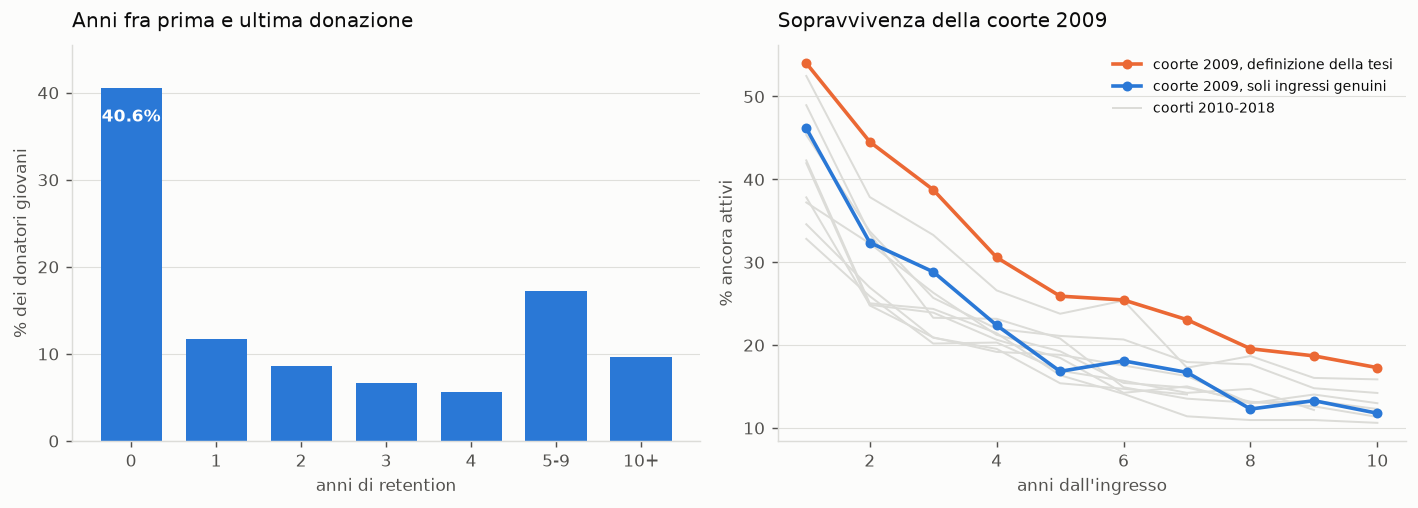
\includegraphics[width=0.95\linewidth]{img/fig_young_retention.png}
    \caption{Sinistra: distribuzione degli anni di retention. Destra:
    sopravvivenza della coorte 2009 sotto le due definizioni, sullo sfondo
    delle coorti 2010--2018.}
    \label{fig:ret_young}
\end{figure}

Quello che invece \textbf{non} cambia è la forma della curva, ed è la
conclusione sostantiva del capitolo: l'abbandono è \emph{frontalmente
caricato}. La perdita più consistente avviene fra il primo e il secondo anno,
e la perdita annua si riduce man mano che il donatore accumula anni. Il
pattern è coerente con una logica a \emph{soglia}: superati i primi anni, il
comportamento tende a stabilizzarsi come abitudine. Dal
punto di vista delle politiche di reclutamento ne segue che l'investimento più
efficace è quello sul \emph{secondo contatto}, cioè sul richiamo dei giovani
già donatori che non si sono ancora ripresentati.

La \cref{fig:ret_byage} mostra che la forma è la stessa per tutte le fasce
d'ingresso: la curva dei 18--25 sta sotto le altre, ma tutte decrescono con lo
stesso profilo frontalmente caricato, con la perdita maggiore fra il primo e il
secondo anno. É la dinamica
dell'ingresso; nei giovani cambia il livello: fa eccezione la
fascia 50+, che parte alta e scende più rapidamente delle altre fino a
incrociarle intorno al sesto anno --- coerentemente con il fatto che chi entra
oltre i cinquant'anni ha comunque davanti un orizzonte di idoneità più breve.

\begin{figure}[H]
    \centering
    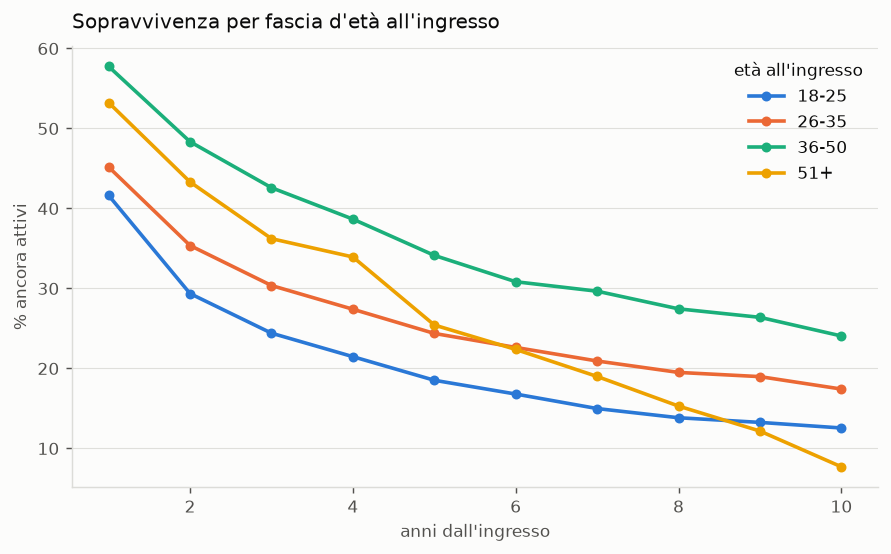
\includegraphics[width=0.90\linewidth]{img/fig_retention_by_age.png}
    \caption{Curve di sopravvivenza per fascia d'età all'ingresso, sui soli
    ingressi genuini.}
    \label{fig:ret_byage}
\end{figure}

% ───────────────────────────────────────────────────────────────────────
\section{Differenze di genere}
\label{sec:ret_gender}

Il gruppo dei donatori giovani è composto da \textbf{5\,786 maschi ($54{,}8\%$)}
e \textbf{4\,766 femmine ($45{,}2\%$)}, un rapporto molto meno squilibrato di
quello della popolazione donante complessiva (M/F $= 1{,}61$,
\cref{sec:demo}): il reclutamento giovanile coinvolge le donne in misura
relativamente maggiore rispetto alle fasce mature.

Le differenze di retention sono modeste ma coerenti (\cref{tab:ret_gender}): i
maschi hanno una retention media leggermente superiore ($3{,}24$ contro
$2{,}84$ anni) e una quota di \emph{one-timer} inferiore ($39{,}6\%$ contro
$41{,}7\%$). In entrambi i generi la mediana è 1 anno e il
75\textsuperscript{o} percentile è 5.

\begin{table}[ht]
\centering
\caption{Retention per genere, donatori giovani (soli ingressi genuini).}
\label{tab:ret_gender}
\begin{tabular}{@{}lrrrrrr@{}}
\toprule
\textbf{Genere} & \textbf{N} & \textbf{Media} & \textbf{DS} &
\textbf{Mediana} & \textbf{P75} & \textbf{One-timer} \\
\midrule
Maschi  (M) & 5\,786 & $3{,}24$ & $4{,}15$ & 1 & 5 & $39{,}6\%$ \\
Femmine (F) & 4\,766 & $2{,}84$ & $3{,}70$ & 1 & 5 & $41{,}7\%$ \\
\midrule
\textbf{Totale} & \textbf{10\,552} & $3{,}06$ & $3{,}96$ & 1 & 5 & $\mathbf{40{,}6\%}$ \\
\bottomrule
\end{tabular}
\end{table}

Il divario di $2{,}1$ punti percentuali è troppo contenuto per giustificare
strategie di retention differenziate per genere. Nelle analisi del
\cref{ch:glm} il genere entra quindi come covariata di controllo, non come
variabile di stratificazione --- il che è anche coerente con il fatto, discusso
nella \cref{sec:glm_effects}, che l'effetto del genere sulla \emph{frequenza} è
in larga parte un vincolo normativo e non una differenza di propensione.

% ───────────────────────────────────────────────────────────────────────
\section{Confronto con i donatori adulti}
\label{sec:ret_comparison}

I \textbf{10\,533 donatori adulti} (ingresso a 26 anni o più) permettono di
contestualizzare il risultato. Qui la correzione della coorte cambia
sensibilmente la conclusione (\cref{tab:ret_fasce}).

\begin{table}[ht]
\centering
\caption{Quota di \emph{one-timer} per fascia d'età all'ingresso, contando
come ingresso il primo evento osservato e contando invece i soli ingressi
genuini.}
\label{tab:ret_fasce}
\begin{tabular}{@{}lrr@{}}
\toprule
\textbf{Fascia d'ingresso} & \textbf{Primo evento oss.} & \textbf{Ingressi genuini} \\
\midrule
18--25 & $39{,}1\%$ & $40{,}6\%$ \\
26--35 & $31{,}1\%$ & $38{,}1\%$ \\
36--50 & $22{,}1\%$ & $28{,}2\%$ \\
51+    & $27{,}7\%$ & $33{,}1\%$ \\
\midrule
\emph{aggregato 26+} & $26{,}2\%$ & $33{,}3\%$ \\
\midrule
\textbf{rapporto giovani\,/\,adulti} & $\mathbf{1{,}49}$ & $\mathbf{1{,}22}$ \\
\bottomrule
\end{tabular}
\end{table}

Il divario esiste ancora --- i giovani abbandonano più spesso degli adulti ---
ma è \textbf{molto più piccolo di quanto la misura ingenua suggerisca}: un
rapporto di $1{,}22$ anziché di $1{,}49$. La ragione è ora evidente: i donatori troncati a sinistra
sono concentrati nelle fasce mature (chi è osservato a 45 anni ha più
probabilità di aver già una carriera alle spalle di chi è osservato a 20), e
sono per costruzione dei sopravvissuti. Confrontare giovani e adulti senza
rimuoverli significa confrontare reclute con veterani e attribuire la
differenza all'età.

Resta valido, e anzi si rafforza, il motivo per cui la retention giovanile
merita uno studio autonomo: sono \textbf{la metà di tutti gli ingressi} e hanno davanti
l'orizzonte di attività più lungo. Perdere un ventenne al primo anno costa al
sistema molto più che perdere un cinquantenne, a parità di tasso di abbandono.

% ───────────────────────────────────────────────────────────────────────
\section{Sintesi e implicazioni per la modellazione}
\label{sec:ret_summary}

\textbf{1. Abbandono precoce maggioritario.}
Il $40{,}6\%$ dei donatori che entrano fra i 18 e i 25 anni non torna negli anni
successivi al primo, e il $52{,}3\%$ abbandona dopo il secondo anno.

\textbf{2. Dinamica a soglia.}
La funzione di rischio è decrescente: il rischio di abbandono è massimo fra la
prima e la seconda donazione e si riduce progressivamente. Chi supera i cinque
anni ha buone probabilità di restare a lungo, il che individua una soglia di
consolidamento dell'abitudine intorno al terzo--quinto anno.

\textbf{3. Il divario con gli adulti è reale ma modesto.}
Un rapporto di $1{,}22$, non di $1{,}5$: gran parte di quello che sembrava un
effetto dell'età era troncamento a sinistra. La ragione per concentrarsi sui
giovani non è che abbandonino molto di più, ma che sono metà degli ingressi e
hanno l'orizzonte più lungo.

\textbf{4. Differenze di genere contenute.}
$2{,}1$ punti percentuali nei \emph{one-timer}: il genere va trattato come
covariata di controllo, non come variabile di stratificazione.

Per il \cref{ch:glm} le implicazioni sono due. La prima è che l'anzianità nel
sistema va controllata esplicitamente, perché è la variabile lungo cui la
popolazione si assottiglia: senza quel controllo qualunque effetto stimato
sull'età anagrafica ne assorbe una parte. La seconda è che un modello di
frequenza che osservi solo gli anni in cui il donatore dona non può vedere
l'abbandono descritto qui --- il che porta direttamente alla scelta dell'unità
di analisi discussa nella \cref{sec:glm_unit}.

% ══════════════════════════════════════════════════════════════════════════════
%  Fine Capitolo — Fidelizzazione dei Donatori Giovani
% ══════════════════════════════════════════════════════════════════════════════


% ══════════════════════════════════════════════════════════════════════════════
%  CAPITOLO — MODELLI DI REGRESSIONE PER CONTEGGI
%  Etichette: ch:glm, sec:glm_unit, sec:glm_spec, sec:glm_overdisp,
%             sec:glm_effects, sec:glm_time, sec:glm_holdout, sec:glm_summary
% ══════════════════════════════════════════════════════════════════════════════

\chapter{Modelli di Regressione per Conteggi}
\label{ch:glm}
Si introducono ora alcuni dei modelli statistici utilizzati per spiegare la 
frequenza di donazione dei singoli donatori, per poi commentare i risultati di
tale analisi. La domanda a cui si cercherà di rispondere è:
``che comportamento assume il singolo donatore? Quali sono
le probabilità che torni a donare?''. La domanda è di tipo inferenziale: a
parità di ogni altra condizione, quali caratteristiche sono associate a una
frequenza di donazione più alta? Quanto esse influiscono sulla frequenza stessa?

La risposta è un conteggio: questa caratteristica di per sé pone un vincolo
sulla classe di modelli che sarà possibile utilizzare.
La regressione lineare ordinaria è inadeguata: nei conteggi la varianza cresce con
la media, mentre in questi tipi di modelli essa è assunta costante.
Si ricorre quindi ai modelli lineari generalizzati per dati di
conteggio~\cite{CameronTrivedi2013}, nelle versioni di Poisson e binomiale
negativa, confrontate nella \cref{sec:glm_overdisp}.

% ───────────────────────────────────────────────────────────────────────
\section{Unità di analisi e variabile risposta}
\label{sec:glm_unit}

La scelta dell'unità di osservazione
determina cosa il modello può vedere. Dopo aver passato al vaglio le possibilità,
se ne sono escluse alcune apparentemente intuitive per le seguenti motivazioni:

\paragraph{Riga evento: }
Il dataset originale è composto riga per evento di donazione; tra le colonne,
è presente \texttt{num\_don}, aggregato di livello
superiore: esso rappresenta il numero di donazioni del gruppo (donatore $\times$ anno $\times$
tipologia) cui la riga appartiene, uguale per ogni riga appartenente a quel gruppo
(\cref{sec:dataset}). Se si stimasse un modello a partire da quelle righe e con \texttt{num\_don}
come variabile risposta, ogni gruppo entra nella verosimiglianza tante volte quante sono
le sue donazioni: più grande è il singolo gruppo e più peso avrà, proporzionalmente
al valore della variabile risposta. La media stimata è quindi distorta, e di conseguenza
anche gli errori standard e ogni test di dispersione. 
% La differenza è misurabile: la media della risposta calcolata
%sulle righe è $2{,}47$, quella calcolata sui gruppi $1{,}70$.

\paragraph{Deduplicazione.}
Una correzione del fenomeno appena descritto è la \textbf{deduplicazione}, ovvero
mantenere una sola riga per gruppo (donatore $\times$ anno $\times$ tipologia).
Ciò fa però insorgere due ulteriori problemi.

Il primo, in ordine di importanza, è che \textbf{la risposta é troncata}: una tripla
esiste solo se quella donazione c'è stata, mentre l'informazione riguardante
gli anni in cui il donatore è rimasto in attivo viene persa. Il modello é
\textbf{cieco} circa l'evento che il \cref{ch:retention} ha mostrato essere il più
frequente di tutti: l'abbandono. E la diagnosi di dispersione ne risente in
modo sostanziale: misurato sui soli anni attivi, il rapporto varianza/media è
$\mathbf{1{,}23}$ (quasi equidispersione); considerando anche gli anni di
inattività,essa diventa $\mathbf{2{,}45}$.

Il secondo è che le osservazioni restano \textbf{raggruppate per donatore}: lo
stesso soggetto compare in molti anni, e le sue osservazioni \textbf{non} sono
indipendenti. Deduplicare elimina la replicazione dentro il gruppo, ma non
questa seconda fonte di dipendenza, che va trattata a parte (si veda il
paragrafo sugli errori standard nella \cref{sec:glm_spec}).

\paragraph{Il grano adottato.}
La risposta è il \textbf{numero di donazioni per donatore e anno, con gli anni
a zero materializzati}: il panel costruito al terzo e ultimo stadio della pipeline
(\cref{sec:cleaning}), composto da \textbf{514\,098 righe}, il $63{,}9\%$ delle quali a
zero. Il campione di stima va dal 2013 in poi
(\textbf{444\,240 righe}, 43\,298 donatori), essendoci incertezza sulla storia dei donatori
nei primi anni osservati (tutti sono considerati "esordienti" nel 2009, primo anno a disposizione).

Così facendo, \textbf{la somma della
risposta su un anno è il totale di quell'anno}. Il modello individuale di
questo capitolo e la previsione aggregata dell'\cref{ch:forecast} misurano
quindi la stessa grandezza e non possono contraddirsi.

% ───────────────────────────────────────────────────────────────────────
\section{Modello GLM per conteggi}
\label{sec:glm_model}
Prima di discutere il modello usato nelle previsioni svolte, si introduce il concetto di
GLM~\cite{McCullaghNelder1989}.

Un \textbf{GLM} (Generalized Linear Model) è un modello statistico definito
da tre componenti principali: 
\begin{itemize}
    \item \textbf{Componente casuale}: com'è distribuita la variabile risposta $\mathbf{Y}$ appartenente
    alla famiglia esponenziale; 
    \item \textbf{Predittore lineare}: costruito nella forma 
    $\eta = \beta_{0} + \beta_{1}x_{1} + \beta_{2}x_{2} + ... + \beta_{n}x_{n}$;
    \item \textbf{Funzione di legame}: collega la media della risposta al predittore: 
    $g(\mu) = \eta,  \mu = \mathbb{E}[\mathbf{Y}]$.
\end{itemize}

\paragraph{GLM di Poisson.} Durante lo studio si è ipotizzato l'utilizzo della \textbf{GLM di Poisson} 
--- essa ha un solo parametro $\lambda$ e si ha:
\begin{equation}
    \mathbb{E}[\mathbf{Y}] = \mathbb{V}[\mathbf{Y}] = \lambda
\end{equation}

Analizzando i dati, si nota come $\mathbb{V}[\mathbf{Y}] \gg \mathbb{E}[\mathbf{Y}]$ (\textbf{sovradispersione}); 
la GLM di Poisson è stata quindi considerata inadatta a descrivere il fenomeno osservato.

\paragraph{GLM Binomiale Negativa.} La \textbf{GLM Binomiale Negativa} è stata quindi
considerata come alternativa; intuitivamente, essa può essere vista come una
\textbf{Poisson}, dove la singola osservazione $i$ ha un proprio \textbf{tasso latente}
$\mu_i u_i$, $u_i$ \textbf{fattore di eterogeneità non osservata} diverso per ogni soggetto,
distribuito secondo una \textbf{Gamma} di media 
$1$ e varianza $\alpha$.
Si ha quindi:
\begin{equation}
    \mathbf{Y}_{i} | u_{i} \sim \text{Po}(\mu_{i}u_{i}), \quad u_{i} \sim \Gamma(1/\alpha, \alpha)
\end{equation}
Integrando per il fattore di eterogeneità $u_i$, si ha:
\begin{equation}
    \mathbb{E}[\mathbf{Y}_{i}] = \mu_{i}, \quad \mathbb{V}[\mathbf{Y}_{i}] = \mu_{i} + \alpha\mu_{i}^{2}
    \implies \mathbf{Y}_{i} \sim \text{NB}(\mu_{i}, \alpha) 
\end{equation}

Questa \textit{parametrizzazione} è detta \textbf{NB2}. $\alpha$ misura la \textbf{sovradispersione} del modello:
se $\alpha=0$, si collassa nella \textbf{Poisson} (caso limite).

\paragraph{Link e forma del modello.} Il terzo elemento della specifica è la
\textbf{funzione di legame}, che in questo caso è il \textbf{logaritmo naturale}:
\begin{equation}
    \ln\mu_i = \ln\mathbb{E}[\mathbf{Y}_i \mid \mathbf{x}_i] = \mathbf{x}_{i}^\top\boldsymbol{\beta}
\end{equation}

Questa scelta è motivata dal fatto che la risposta è un conteggio, quindi non può assumere valori negativi;
il modello avrà quindi la stessa forma della media di un GLM di Poisson, ma con una varianza più flessibile: 
ciò lo rende più fedele e adatto ai dati osservati che presentano la sovradispersione discussa in precedenza.

\paragraph{Stima dei parametri.}
Solitamente la stima dei parametri $\beta$ e $\alpha$ avviene tramite il 
\textbf{metodo della massima verosimiglianza} (MLE).

$\alpha$ può essere stimato anche con il \textbf{metodo dei momenti}: si stima
prima il modello di Poisson, che fornisce le medie $\hat{\mu}_i$, e si sceglie
$\alpha$ in modo che la relazione $\mathbb{V}[Y_i] = \mu_i + \alpha\mu_i^2$ valga
in media sui residui,
\begin{equation}
    \hat{\alpha} = \frac{1}{n}\sum_{i=1}^{n}
    \frac{(y_i - \hat{\mu}_i)^2 - \hat{\mu}_i}{\hat{\mu}_i^2}.
\end{equation}
Nel modello utilizzato nelle analisi $\alpha$ è stato stimato con quest'ultimo
metodo e poi fissato come costante: $\hat{\alpha} = 2{,}37$.
% ───────────────────────────────────────────────────────────────────────

\section{Specificazione}
\label{sec:glm_spec}

Il modello ha forma
\begin{equation}
    \log \mathbb{E}[Y_{it} \mid \mathbf{x}_{it}]
    = \beta_0
    + \beta_{\text{a}}\,\text{età}_{it}
    + \beta_{\text{c}}\,\text{carriera}_{it}
    + \beta_{\ell}\,\text{troncato}_{i}
    + \boldsymbol{\gamma}^\top \mathbf{d}_{it}
    + \delta\,(\text{anno}_t - 2016),
    \label{eq:glm_form}
\end{equation}
dove $i$ indicizza il donatore e $t$ l'anno, e $\mathbf{d}_{it}$ raccoglie le
variabili categoriche. Con legame logaritmico ogni coefficiente esponenziato si
interpreta come \emph{Incidence Rate Ratio} (IRR): il rapporto fra il numero
atteso di donazioni con e senza la caratteristica, tenute ferme le altre.

Si pone particolare attenzione ad alcune scelte di specifica:

\paragraph{Carriera.}
La variabile \texttt{carriera} è il numero di anni trascorsi dall'inizio
dell'attività donazionale, misurato sulla data di inizio attività registrata
nel dato grezzo (\texttt{first\_activity\_date}) e, dove questa manca, sul primo
anno osservato. Misurarla dal primo anno osservato farebbe sembrare esordienti
i donatori già attivi prima del 2009. La variabile \texttt{troncato} marca i
donatori la cui carriera risulta iniziata prima del loro primo anno osservato:
per loro la storia donazionale precedente (tipologia, frequenza) non è nel
dataset, anche se l'anzianità è nota.

Senza il controllo per la carriera, un'eventuale coorte di ingresso ne
assorbirebbe l'effetto. Nella variante che aggiunge la coorte quinquennale di
ingresso le coorti recenti hanno IRR crescenti, fino a $3{,}5$ per quella del
2025 e fino a $4{,}0$
se si toglie anche la carriera. Misurano il fatto che quei donatori sono osservati soltanto nei loro primi
anni, che sono quelli con maggiore attività.

\paragraph{Categorie di riferimento esplicite.}
Le categorie di riferimento sono imposte, non ereditate dall'ordinamento
alfabetico: \textbf{P} (periodico) per la classe donatore e \textbf{SANGUE} per
la tipologia, cioè le categorie modali. Ogni IRR si legge così come confronto
con il donatore tipico, e l'intervallo di confidenza è calcolato rispetto a una
base ampia. Le categorie rare della classe donatore (la classe A compare una
volta sola in diciassette anni) non entrano nel campione di stima.

\paragraph{Tipologia ritardata agli anni precedenti.}
Al grano donatore-anno la tipologia dell'anno corrente è un attributo della
risposta: entra quindi la tipologia \emph{prevalente negli anni
precedenti}, che è causale per costruzione.

\paragraph{Una specifica non identificata.}
Un limite strutturale fondamentale è il seguente:
\textbf{età, periodo e coorte di ingresso non sono identificabili insieme}, 
perché anno $=$ anno di ingresso $+$ anni di carriera. Una specifica
che li contenga tutti e tre stima coefficienti identificati soltanto dalla
forma funzionale imposta, come il quinquennio usato come coorte, e non dai dati
stessi. Il modello principale che viene usato
esclude quindi la coorte come cooefficiente.

\paragraph{Errori standard.}
Tutti gli errori standard riportati sono \textbf{robusti per cluster di
donatore}: non c'è assunzione di indipendenza tra entry dello stesso soggetto
in anni differenti.

% ───────────────────────────────────────────────────────────────────────
\section{Sovradispersione e scelta della distribuzione}
\label{sec:glm_overdisp}

Il modello facente uso della distribuzione di Poisson impone 
$\mathbb{E}[Y] = \mathrm{Var}[Y]$. Sul panel
completo, la risposta ha media $0{,}69$ $\neq$ varianza $1{,}68$, con
varianza/media $\mathbf{2{,}45}$: è evidente la sovradispersione del modello.

Il modello binomiale negativo non ha vincoli, in quanto introduce un parametro di
dispersione $\alpha$:
\begin{equation}
    \mathrm{Var}[Y] = \mu + \alpha\,\mu^2 .
    \label{eq:nb_var}
\end{equation}
Come anticipato nella \cref{sec:glm_model}, la stima ottenuta tramite il metodo dei momenti
è $\hat{\alpha} = 2{,}37 \gg 0$.
Questo valore, anziché venire ristimato, entra nel
modello come costante. Di conseguenza i due
modelli hanno lo stesso numero di parametri e la binomiale negativa non
subisce una penalizzazione per il parametro $\alpha$; con una differenza di AIC di sei cifre il punto è
irrilevante per la conclusione, ma va detto. Il confronto sui criteri di informazione
(\cref{tab:glm_fit}) è netto: la differenza di AIC è di \textbf{115\,936 punti}
a favore del modello binomiale negativo.

\begin{table}[ht]
\centering
\caption{Adattamento dei due modelli sul panel donatore-anno (444\,240
osservazioni).}
\label{tab:glm_fit}
\begin{tabular}{@{}lrrr@{}}
\toprule
\textbf{Modello} & \textbf{AIC} & \textbf{BIC} & \textbf{Log-veros.} \\
\midrule
Poisson                   & 986\,075{,}9 & 986\,196{,}9 & $-493\,026{,}9$ \\
Binomiale negativo        & \textbf{870\,140{,}3} & \textbf{870\,261{,}3} & $\mathbf{-435\,059{,}1}$ \\
\midrule
Differenza                & $115\,935{,}6$ & $115\,935{,}6$ & $57\,967{,}8$ \\
\bottomrule
\end{tabular}
\end{table}

Su una tabella deduplicata e ristretta a una singola annualità, quindi,
la binomiale negativa collassa
sulla Poisson, e la sovradispersione sembra svanire  (\cref{sec:dash_overdisp}). La verifica appena svolta
mostra che quell'esito era un artefatto del troncamento: osservando i soli anni attivi,
si osserva una popolazione già selezionata, a cui sono già stati rimossi gli zeri.
Con gli zeri al loro posto, la sovradispersione è massiccia e la scelta della
binomiale negativa non è in discussione.

Tutti i risultati che seguono si riferiscono al modello binomiale negativo.

% ───────────────────────────────────────────────────────────────────────
\section{Effetti stimati}
\label{sec:glm_effects}

\begin{table}[ht]
\centering
\caption{Modello binomiale negativo al grano donatore-anno: IRR, intervalli di
confidenza al 95\% con errori standard robusti per cluster di donatore, e
$p$-value. È omesso il livello residuale \textsc{altro} della tipologia
pregressa, troppo raro per essere stimato con precisione (IRR $0{,}78$,
$p = 0{,}61$).}
\label{tab:glm_irr}
\begin{tabular}{@{}lrrl@{}}
\toprule
\textbf{Termine} & \textbf{IRR} & \textbf{IC 95\%} & \textbf{$p$} \\
\midrule
\multicolumn{4}{@{}l}{\emph{Caratteristiche del donatore}} \\
Genere F (rif.\ M)          & $\mathbf{0{,}585}$ & $[0{,}566;\ 0{,}605]$ & $<0{,}001$ \\
Età (per anno)              & $1{,}0007$ & $[0{,}9994;\ 1{,}0020]$ & $0{,}31$ \\
Anni di carriera (per anno) & $0{,}980$  & $[0{,}977;\ 0{,}983]$ & $<0{,}001$ \\
Carriera troncata a sinistra& $0{,}907$  & $[0{,}866;\ 0{,}951]$ & $<0{,}001$ \\
\addlinespace
\multicolumn{4}{@{}l}{\emph{Classe donatore all'ingresso} (rif.\ P --- periodico)} \\
D --- prima donazione       & $0{,}786$  & $[0{,}751;\ 0{,}821]$ & $<0{,}001$ \\
O --- occasionale           & $0{,}490$  & $[0{,}470;\ 0{,}512]$ & $<0{,}001$ \\
\addlinespace
\multicolumn{4}{@{}l}{\emph{Tipologia prevalente pregressa} (rif.\ SANGUE)} \\
AFPLTPLASM                  & $2{,}194$  & $[1{,}862;\ 2{,}586]$ & $<0{,}001$ \\
PLASMAF                     & $\mathbf{1{,}766}$ & $[1{,}660;\ 1{,}879]$ & $<0{,}001$ \\
\addlinespace
\multicolumn{4}{@{}l}{\emph{Tempo}} \\
Anno (rispetto al 2016)     & $0{,}941$  & $[0{,}938;\ 0{,}943]$ & $<0{,}001$ \\
\midrule
Dispersione $\hat{\alpha}$  & \multicolumn{3}{l}{$2{,}37$} \\
\bottomrule
\end{tabular}
\end{table}

\paragraph{Genere.}
È l'effetto più netto del modello. A parità di ogni altra condizione, le
donatrici (F) registrano una frequenza attesa inferiore rispetto ai donatori (M),
pari al $\mathbf{58{,}5\%}$ di quella
dei donatori maschi. La motivazione è da ricercare nella normativa italiana~\cite{dm2015},
che impone alle donne in età fertile un intervallo minimo fra donazioni di sangue intero più
lungo e un numero massimo annuo inferiore (due contro quattro), a cui si aggiunge la
maggiore frequenza di sospensioni per anemia. \textbf{É quindi un vincolo regolamentare e normativo},
interpretarlo altrimenti sarebbe un errore sostanziale.

\paragraph{Età e anzianità.}
L'effetto dell'età anagrafica è \textbf{statisticamente indistinguibile da
zero} ($p = 0{,}31$), mentre quello dell'anzianità di carriera è netto e
negativo: $-2\%$ di frequenza attesa per ogni anno trascorso dall'inizio
dell'attività. Poiché l'età è già nel modello, questo calo non può essere
attribuito all'invecchiamento o all'uscita dai limiti di età: riflette il fatto
che il panel tiene ogni donatore anche dopo che ha smesso, e che al crescere
degli anni di carriera cresce la probabilità di averlo già fatto. È, letta al
grano donatore-anno, la stessa perdita progressiva descritta nel
\cref{ch:retention}.

Il risultato sull'età dipende interamente dal controllo per anzianità.
Togliendolo dalla specifica, l'età riemerge con un IRR di $0{,}9963$
($-0{,}4\%$ per anno d'età) e un $p$-value inferiore a $0{,}001$ --- un
effetto apparentemente solido. Senza quel controllo il coefficiente dell'età
sta misurando l'anzianità: a parità di anno, i donatori più anziani hanno in
media carriere più lunghe, quindi più anni trascorsi dall'ingresso e più
probabilità di avere già smesso, e il modello attribuisce all'età ciò che
appartiene alla carriera.

\paragraph{Classe donatore, e una rottura di codifica.}
L'ordinamento stimato è quello atteso (periodico $>$ prima donazione $>$
occasionale): un donatore entrato come occasionale
dona meno della metà di uno entrato come periodico, con intervalli stretti ---
il che, come detto sopra, dipende dall'aver imposto \textbf{P} come
riferimento anziché ereditarlo.

Sulla variabile grava però un problema di fondo: \textbf{la classe donatore
cambia codifica nel 2016}. La classe O passa da circa 3\,000
casi l'anno a una decina fra il 2015 e il 2017, e contemporaneamente compare
la classe D, prima inesistente (\cref{fig:donor_class_regime}).

\begin{figure}[H]
    \centering
    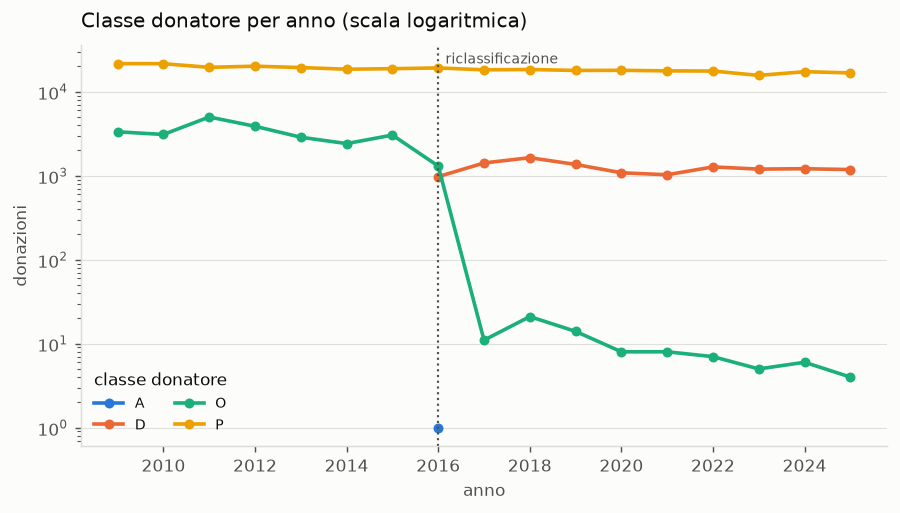
\includegraphics[width=0.9\linewidth]{img/fig_donor_class_regime.png}
    \caption{Donazioni per classe donatore e anno, scala logaritmica. La
    discontinuità del 2016 è una riclassificazione amministrativa.}
    \label{fig:donor_class_regime}
\end{figure}

È una riclassificazione amministrativa.
Nel modello la variabile entra come \emph{classe all'ingresso}, che
attenua il problema ma non lo elimina. L'ordinamento
stimato va quindi letto come robusto nella direzione ma non come una misura
comparabile fra i due regimi, e l'assunzione ``D $=$ prima donazione'' andrebbe
verificata direttamente con il DIMT prima di essere data per buona.

\paragraph{Tipologia di donazione.}
Chi ha donato prevalentemente plasma continua a donare $1{,}77$ volte più
spesso di chi ha donato prevalentemente sangue intero. Ciò é dovuto, come altre
statistiche, ad una questione di regolamentazioni: il plasma è ricostituito in giorni
anziché in settimane, e l'intervallo minimo fra due plasmaferesi è di 14 giorni
contro i 90 del sangue intero~\cite{dm2015}.

% ───────────────────────────────────────────────────────────────────────
\section{Andamento temporale}
\label{sec:glm_time}

Il termine temporale è negativo e netto: a profilo fissato la frequenza attesa
scende del $5{,}9\%$ all'anno (\cref{fig:glm_trend}).

\begin{figure}[H]
    \centering
    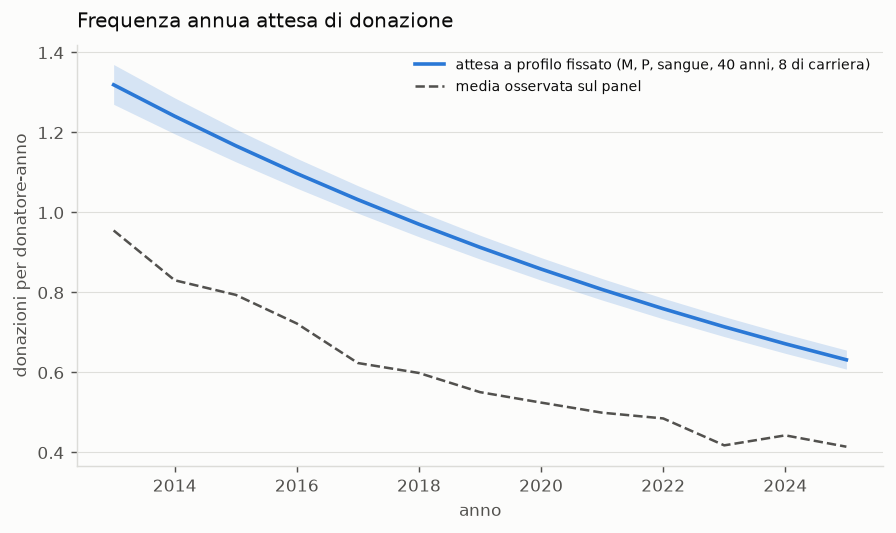
\includegraphics[width=0.95\linewidth]{img/fig_glm_trend.png}
    \caption{Frequenza annua attesa di donazione secondo il modello binomiale
    negativo, a profilo fissato (maschio, classe P, sangue intero, 40 anni,
    otto anni di carriera), con intervallo di confidenza al 95\%; in
    tratteggio, la media osservata sul panel.}
    \label{fig:glm_trend}
\end{figure}

Il valore va letto con attenzione, perché è più ripido del calo aggregato del
\cref{ch:eda} ($-28\%$ in diciassette anni): il panel accumula donatori, compresi gli
occasionali o chi interrompe l'attività di donazione,
quindi la sua composizione si sposta di anno in anno verso i dormienti. La
frequenza media \emph{per riga di panel} cala per questo motivo oltre che per
un'eventuale riduzione di attività dei donatori vivi.

Ciononostante, il risultato sostantivo resta lo stesso:
\textbf{l'intensità individuale attesa non sta crescendo}. Non c'è, nei dati, 
la compensazione da parte dei donatori esistenti
che avrebbe potuto tenere stabile il volume aggregato --- coerentemente con
quanto già osservato nella \cref{sec:intensity}, dove il numero medio di
donazioni per donatore attivo si rivela piatto lungo tutti i diciassette anni.
Quanto questo sia preoccupante dipende anche dalla domanda: se nello stesso
periodo il fabbisogno di emocomponenti del territorio fosse calato, una raccolta
più piccola potrebbe restare adeguata. È una verifica che richiede i dati di
consumo, che questo lavoro non ha.

% ───────────────────────────────────────────────────────────────────────
\section{Verifica predittiva}
\label{sec:glm_holdout}

L'AIC misura l'adattamento in campione e premia il modello più flessibile. Per
una verifica indipendente serve una divisione dei dati, che va
scelta coerentemente all'uso del modello.

Una divisione \emph{casuale} sulle righe non è adeguata qui, per due
ragioni cumulative:
\begin{itemize}
    \item la correlazione: donazioni dello stesso soggetto potrebbero finire
 sia in addestramento che in verifica;
    \item dati \emph{temporali}: le donazioni sono posizionate sulla linea del tempo e,
mischiandole casualmente, una donazione avvenuta nel 2011 potrebbe finire nel test,
mentre una del 2024 nel training set.
\end{itemize}


La verifica corretta è quella temporale: si stima su tutto ciò che precede
un'origine e si valuta su ciò che segue. È il criterio applicato
sistematicamente nell'\cref{ch:forecast}, dove i modelli per donatore di questo
capitolo sono confrontati con gli altri candidati sullo stesso backtest a
origine mobile. L'esito, riportato nella \cref{tab:fc_backtest}, è piuttosto significativo:
\textbf{i modelli per donatore, sommati per ottenere il volume aggregato,
sbagliano circa il doppio del trend smorzato} ($6{,}5\%$ contro $3{,}5\%$ di
MAPE), e la causa è identificata nella \cref{sec:fc_volume}.

Questo non annulla lo studio eseguito, ma ne circoscrive l'utilizzo: il modello appena descritto
serve a \emph{spiegare} la frequenza donazionale e per quello i suoi
coefficienti sono informativi. Non è lo strumento migliore per \emph{prevedere}
il volume aggregato.

% ───────────────────────────────────────────────────────────────────────
\section{Sintesi e limiti}
\label{sec:glm_summary}

\paragraph{1. I vincoli clinici pesano sul comportamento.}
Due degli effetti più forti e più precisi, genere (IRR $0{,}585$) e tipologia
prevalente (IRR $1{,}77$ per la plasmaferesi), misurano in larga parte la
regolamentazione: intervalli minimi fra donazioni e tetti annui differenziati.
Qualunque politica di intensificazione della raccolta deve partire da qui: il
margine di manovra sui donatori esistenti è vincolato in alto da regole
cliniche, non dalla loro disponibilità.

\paragraph{2. L'anzianità di sistema conta, l'età anagrafica no.}
Controllando per gli anni di carriera, l'effetto dell'età anagrafica sparisce
($p = 0{,}31$). Ciò che distingue un donatore assiduo non è quanti anni ha, ma
da quanto tempo dona --- il che rafforza la lettura del \cref{ch:retention}: il
valore di un donatore si costruisce nel tempo, e perderlo presto costa molto
più di quanto suggerisca il conteggio delle donazioni mancate nel primo anno.

\paragraph{Limiti.}
\textbf{Età, periodo e coorte non sono identificabili insieme:} il modello
principale esclude la coorte di ingresso per questo motivo, e la variante che
la include produce coefficienti identificati dalla forma funzionale:
separare effetto di età ed effetto di coorte richiede
un'assunzione esterna che qui non si è voluta imporre. \textbf{Manca una
struttura longitudinale esplicita:} gli errori standard robusti per cluster
tengono conto della correlazione fra anni dello stesso donatore, ma il
modello non stima un effetto individuale, e un modello a effetti casuali sul
donatore sarebbe la specifica più ricca e lo sviluppo naturale di questo
capitolo. Pesa inoltre \textbf{la rottura di codifica di
\texttt{donor\_class}} discussa nella \cref{sec:glm_effects}: la variabile
confronta due schemi amministrativi diversi, e l'ordinamento va letto come
robusto nella direzione ma non nella scala. Infine il modello \textbf{non ha
interazioni}: è puramente additivo e non può cogliere, ad esempio, che il
divario di genere sia diverso fra sangue intero e plasmaferesi, ipotesi
plausibile dato che i tetti normativi differiscono per tipologia.

% ══════════════════════════════════════════════════════════════════════════════
%  Fine Capitolo — Modelli di Regressione per Conteggi
% ══════════════════════════════════════════════════════════════════════════════



%*******************************************************
% Capitolo conclusivo
%*******************************************************
\chapter{Conclusioni}
\label{ch:conclusioni}

Questa tesi ha ricostruito diciassette anni di attività donazionale del DIMT
di Trieste e Gorizia --- 353\,671 donazioni di 43\,299 donatori, dal 2009
al 2025 --- per stimare quanto sangue il sistema
può attendersi di raccogliere, e da chi. Le due province coprono circa un
quinto del bacino donazionale del Friuli Venezia Giulia e non ne riproducono
le caratteristiche; le conclusioni che seguono vanno lette come relative al
territorio osservato.

\section*{Cosa si è trovato}

\textbf{Il sistema si contrae.} Il volume annuale
cala del $28{,}1\%$ fra il 2009 e il 2025, con la flessione concentrata nella
prima metà del periodo e un assestamento successivo. Rapportando le donazioni
alla popolazione residente di Trieste e Gorizia in età donabile --- una
scomposizione che questo lavoro introduce e che la sola serie assoluta non
consente --- si ottiene che il calo demografico spiega solo il $12{,}2\%$
della contrazione, mentre il restante $87{,}8\%$ è imputabile alla perdita di partecipazione. 

\textbf{Il fronte critico è contenuto in una fascia d'età.} A parità di popolazione
i 20--24enni sono la fascia con il tasso di donazione più alto in ogni anno
osservato, e costituiscono metà di tutti gli ingressi. Le fasce che crollano
sono le 35--44, che perdono fra il 36 e il 41 per cento del tasso di
partecipazione, mentre in corrispondenza delle fasce 55--64 si raggiunge uno stallo. 
Nel 2009 il profilo per età mostra un altopiano fra i 35 e i 49 anni,
che sparisce nel 2025. Il sistema, quindi,
non ha perso le nuove leve, ma i donatori di mezza età.

\textbf{Mantenere i giovani all'interno del sistema è difficile.} 
Il $40{,}6\%$ dei donatori che
entra fra i 18 e i 25 anni non dona più dopo il primo anno, e il
$52{,}3\%$ smette dopo il secondo. Il divario rispetto a chi entra più
tardi esiste ma è modesto --- rapporto di $1{,}22$ anziché $1{,}5$ --- una
volta rimossi dal confronto i donatori intercettati a metà carriera, che per
costruzione sono dei sopravvissuti. La funzione di rischio è decrescente:
superati i primi anni, il comportamento donazionale si consolida.

\textbf{Il margine sui donatori già attivi è vincolato.} I due effetti più
forti del modello di frequenza --- genere e tipologia di donazione --- sono
frutto di paletti regolamentari: intervalli minimi fra donazioni e
tetti annui differenziati per sesso. E controllando per gli anni di carriera, si
nota ciò che distingue un donatore assiduo è da
quanto tempo dona, indipendentemente dall'età anagrafica. 
Coerentemente, l'intensità individuale non cresce: le
donazioni per donatore attivo restano fra $1{,}84$ e $1{,}97$ per tutti e
diciassette gli anni.

\section*{Cosa significa operativamente}

I quattro punti convergono su un'indicazione unica. Il volume non si difende
chiedendo di più a chi già dona, perché quel margine è chiuso in alto da regole
cliniche e non da mancanza di disponibilità. Si difende agendo sul \emph{numero} di
donatori, e si può fare in due maniere:

\begin{enumerate}
    \item \textbf{secondo contatto}: quasi metà dei giovani che donano una
volta non torna, ed è qui dove si massimizza il rischio di abbandono . Un
richiamo rivolto a chi ha donato una volta e non si è ripresentato agisce sul
momento in cui la perdita è più probabile e in cui il valore recuperato ---
decenni di carriera potenziale --- è massimo.
    \item \textbf{rientro della fascia di mezza età}, che è il punto dove
la perdita si è effettivamente verificata. Chi ha smesso di donare a quarant'anni è,
a differenza di un neodonatore, una persona conosciuta dal sistema, 
che ha già superato la selezione clinica e che ha una storia donazionale registrata.
È il bacino su cui un'azione di richiamo ha il costo di contatto più basso.
\end{enumerate}

La proiezione al 2031 --- circa 97\,200 donazioni complessive nel sessennio,
con un primo anno più basso del 2025 e poi un calo di poco meno di un punto
percentuale l'anno --- va letta in questa
chiave: è la risposta alla domanda ``cosa succede se nulla cambia'', non una
previsione di ciò che accadrà. Il suo valore è di fissare la linea di base
rispetto a cui misurare un intervento.

\section*{Cosa non si è potuto stabilire}

La domanda aperta più rilevante riguarda le fasce 35--44: se il loro crollo sia
un effetto di \emph{età} o di \emph{coorte}. Se le generazioni oggi
quarantenni hanno sempre donato meno delle precedenti, il fenomeno è
generazionale e si sposterà con loro; se invece hanno donato e hanno smesso, è
recuperabile. Le due letture portano a politiche diverse, e i dati permettono
di porre la domanda ma non, attualmente, di trovarne una risposta: come discusso nella
\cref{sec:glm_spec}, età, periodo e coorte non sono identificabili
simultaneamente senza un'assunzione esterna. Il panel donatore-anno costruito
qui è lo strumento adatto ad affrontarla, ma va detto che i dati raccolti
finora non offrono nemmeno un indizio utilizzabile: nella variante del modello
che include la coorte di ingresso, i coefficienti \emph{crescono} verso le
generazioni più recenti, il che non depone per una minore propensione
generazionale --- riflette piuttosto il fatto che quelle coorti sono osservate
soltanto nei loro primi anni, che sono i più attivi. È la ragione per cui il
\cref{ch:glm} rifiuta di leggerlo come effetto generazionale.

\section*{Un'osservazione sul metodo}

Le conclusioni di questa tesi dipendono, in misura
sorprendente, da tre scelte facilmente classificabili come "tecniche":
quale delle due colonne disponibili identifichi il donatore; se un campo
amministrativo compilato in modo disomogeneo fra le sedi sia un requisito di
ammissione o una covariata; e su quale unità di osservazione si misuri un
conteggio.

Nessuna delle tre è una questione statistica quanto amministrativa,
ma tutte, in base alla scelta presa da chi svolge lo studio, hanno la
possibilità di cambiare i risultati finali. In particolare la seconda
aveva il potere di, essenzialmente, \textit{eliminare} un terzo delle
donazioni isontine --- perché la compilazione di quel campo è una prassi 
di sede, non un attributo del donatore.


% Non modificare questa parte
\appendix
\crefalias{chapter}{appendix}
\cleardoublepage
\phantomsection
\addcontentsline{toc}{part}{Appendici}
\part*{Appendici}
\renewcommand{\chaptermark}[1]{\markboth{\MakeUppercase{\appendixname\ \thechapter.\ #1}}{}}
% Non modificare questa parte

% ══════════════════════════════════════════════════════════════════════════════
%  CAPITOLO — PROIEZIONI 2026-2031
%  Etichette: ch:forecast, sec:fc_data, sec:fc_models, sec:fc_choice,
%             sec:fc_volume, sec:fc_type, sec:fc_donors, sec:fc_summary
% ══════════════════════════════════════════════════════════════════════════════

\chapter{Proiezioni 2026--2031}
\label{ch:forecast}

Il \cref{ch:eda} ha mostrato un volume donazionale in contrazione del $28\%$ in
diciassette anni, con ingressi in calo e intensità individuale ferma; il
\cref{ch:retention} ha quantificato quanto rapidamente si perdono i donatori
dopo il primo contatto. Questa appendice proietta quegli andamenti in avanti di
sei anni, dal 2026 al 2031, per rispondere a una domanda operativa: quante
donazioni può ragionevolmente attendersi il sistema, e con quale margine di
incertezza.

A differenza del \cref{ch:glm}, che modella il comportamento del singolo
donatore per spiegare chi dona di più e perché, qui l'unità di analisi è il
volume aggregato e l'obiettivo non è inferenziale ma predittivo.

% ───────────────────────────────────────────────────────────────────────
\section{Serie storica e criterio di valutazione}
\label{sec:fc_data}

La serie di base è il conteggio mensile 2009--2025 ottenuto per aggregazione
diretta del dataset finale: 204 mesi per \textbf{353\,671 donazioni}
(\cref{fig:fc_monthly}). La struttura è quella descritta nella
\cref{sec:temporal} --- trend decrescente non lineare, stagionalità mensile
contenuta, uno shock esogeno di ampiezza modesta nel 2020.

\begin{figure}[H]
    \centering
    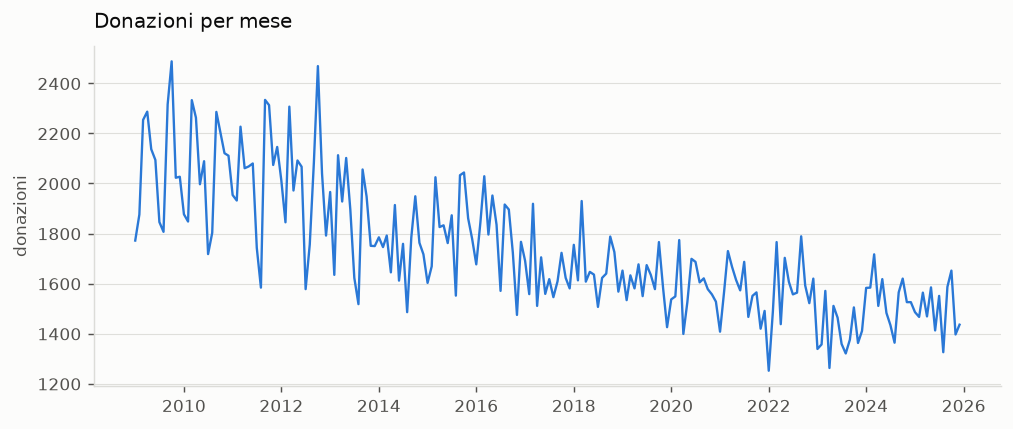
\includegraphics[width=0.95\linewidth]{img/fig_forecast_monthly_history.png}
    \caption{Serie mensile delle donazioni, 2009--2025.}
    \label{fig:fc_monthly}
\end{figure}

\paragraph{Come si confrontano i modelli.}
Il criterio adottato è un \textbf{backtest a origine mobile}: si sceglie un
anno origine $O$, si stima ogni modello sui soli dati fino a $O$, si prevedono
gli anni successivi e si confronta con l'osservato; poi si sposta l'origine in
avanti e si ripete. Con nove origini e orizzonti da uno a tre anni si ottengono
ventiquattro coppie (previsione, osservato) per ciascun candidato, tutte sugli
stessi anni bersaglio. L'orizzonte è limitato a tre anni perché è il massimo su
cui i modelli per donatore restano stimabili su tutte le origini; le baseline,
che non hanno questo vincolo, sono valutate a parte fino a sei anni --- ed è da
quel confronto, non da questo, che vengono la scelta di $\varphi$
(\cref{sec:fc_choice}) e gli intervalli empirici.

\paragraph{Come si produce una previsione.}
A ogni origine la previsione è \emph{a più passi}: il modello, stimato una
volta sui dati fino a $O$, produce in un colpo solo i valori di
$O+1, \dots, O+h^*$, senza essere aggiornato con l'osservato degli anni
intermedi (la previsione del 2019 fatta dall'origine 2016 non sa nulla del
2017 e del 2018, per esempio). Il metodo di estrapolazione dipende dalla famiglia
(\cref{sec:fc_models}). Le \textbf{baseline} sono formule chiuse sulla serie
annuale: la naive ripete l'ultimo anno, il trend smorzato prolunga una retta
stimata sulla storia con pendenza decrescente (\cref{eq:damped}). Il
\textbf{GLM mensile} prevede i $12h^*$ mesi successivi prolungando il termine
di trend e ripetendo il profilo stagionale stimato, e i mesi si sommano per
anno solare. I \textbf{modelli per donatore} non prevedono il totale ma lo
costruiscono: partendo dallo stato di ogni donatore a fine $O$, si simula un
anno alla volta quante volte ciascuno dona; l'esito simulato di un anno
aggiorna le covariate dell'anno successivo (tempo dall'ultima donazione, anni
di carriera) e ad ogni anno si aggiunge un contingente di nuovi donatori, la cui
numerosità è prevista a parte con un trend smorzato sulla serie degli
ingressi. Il totale che ne risulta è la media di venti percorsi simulati.

La procedura è riassunta nell'\cref{alg:backtest}. Il punto che conta è la
riga~4: la storia passata a ogni modello si ferma all'origine, quindi nessuna
previsione può usare informazione che al momento di produrla non esisteva. È la
sola garanzia che gli errori misurati siano errori di previsione e non di
adattamento.

\begin{algorithm}[H]
\caption{Backtest a origine mobile con finestra espansiva}
\label{alg:backtest}
\begin{algorithmic}[1]
\Require serie $y_{1:T}$; insieme di modelli $\mathcal{M}$; addestramento minimo
$m$; orizzonte massimo $H$
\Ensure una riga $(\text{modello}, O, h, y, \hat{y})$ per ogni valutazione
\State $R \gets \emptyset$
\For{$O = m$ \textbf{fino a} $T-1$}
  \Comment{ogni anno utilizzabile diventa un'origine}
  \State $\text{storia} \gets y_{1:O}$
  \Comment{\textbf{solo} il passato: qui si evita il leakage}
  \ForAll{$f \in \mathcal{M}$}
    \State $\hat{y}_{1:h^*} \gets f(\text{storia},\ h^*)$ \quad con
    $h^* = \min(H,\ T-O)$
    \For{$h = 1$ \textbf{fino a} $h^*$}
      \State $R \gets R \cup \{(f,\ O,\ h,\ y_{O+h},\ \hat{y}_h)\}$
    \EndFor
  \EndFor
\EndFor
\State \Return $R$
\Comment{MAPE, bias e percentili si aggregano da $R$, per modello o per orizzonte}
\end{algorithmic}
\end{algorithm}

\begin{table}[H]
\centering
\small
\caption{Simboli dell'\cref{alg:backtest} e valori adottati.}
\label{tab:backtest_simboli}
\begin{tabularx}{\linewidth}{@{}l X l@{}}
\toprule
\textbf{Simbolo} & \textbf{Significato} & \textbf{Valore} \\
\midrule
$y_t$ & donazioni osservate nell'anno $t$ & --- \\
$y_{1:T}$ & serie annuale completa & 2009--2025 \\
$T$ & numero di anni della serie & 17 \\
$\mathcal{M}$ & insieme dei modelli candidati & 17 \\
$f$ & un modello di $\mathcal{M}$: riceve la storia e un orizzonte, restituisce le previsioni & --- \\
$m$ & addestramento minimo, in anni, prima della prima origine & 8 \\
$H$ & orizzonte massimo di previsione & 3 (6 baseline) \\
$O$ & origine: ultimo anno usato per la stima & 2016--2024 \\
storia & dati disponibili all'origine, $y_{1:O}$ & --- \\
$h$ & orizzonte: distanza in anni dall'origine & $1,\dots,h^*$ \\
$h^*$ & orizzonte effettivo $\min(H,\,T-O)$, ridotto per le ultime origini & 3, 2 o 1 \\
$\hat{y}_h$ & previsione per l'anno $O+h$ fatta all'origine $O$ & --- \\
$y_{O+h}$ & valore osservato nello stesso anno & --- \\
$R$ & insieme dei risultati, una riga per valutazione & 24 per modello \\
\bottomrule
\end{tabularx}
\end{table}

Poiché ogni modello riceve le stesse origini e gli stessi bersagli, il confronto
della \cref{tab:fc_backtest} non dipende da quale periodo sia capitato a chi.
Dallo stesso insieme $R$ si ricavano, filtrando sul modello adottato e
raggruppando per orizzonte, i percentili che formano gli intervalli della
\cref{sec:fc_choice}.

La differenza rispetto a una singola divisione non è pedanteria. Con una sola
divisione il giudizio dipende da quale periodo è finito nel campione di
verifica: se contiene un evento eccezionale, si sta misurando quanto un modello
è fortunato, non quanto è accurato. Con nove origini l'evento eccezionale entra
in alcune finestre e non in altre, e il confronto diventa informativo. Va
segnalato che questo criterio è più severo del precedente: gli errori riportati
qui sotto sono più alti di quelli che si otterrebbero su un holdout singolo
favorevole, e sono la stima onesta.

% ───────────────────────────────────────────────────────────────────────
\section{Confronto tra approcci di modellazione}
\label{sec:fc_models}

Sono stati confrontati diciassette candidati, divisi in tre famiglie che
differiscono per ciò che modellano. Le \textbf{baseline} (nove) lavorano sulla
serie annuale con formule elementari: ultimo anno ripetuto, media degli ultimi
tre o cinque anni, trend lineare, trend smorzato con $\varphi \in \{0{,}6;\
0{,}7;\ 0{,}8\}$ e una media fra trend smorzato e media mobile. I
\textbf{modelli sulla serie aggregata} (due) sono GLM quasi-Poisson sulla serie
mensile, con effetti di mese e un trend lineare o a spline, e le previsioni
mensili si sommano per anno. I \textbf{modelli per singolo donatore} (sei) non
sono modelli di serie storiche: sono regressioni per conteggi sul panel
donatore-anno --- Poisson, binomiale negativa, hurdle, con e senza trend, e un
LightGBM con perdita di Poisson --- e il totale annuo si ottiene simulando ogni
donatore e sommando (\cref{sec:fc_data}). La \cref{tab:fc_backtest} riporta i
principali.

\begin{table}[ht]
\centering
\caption{Backtest a origine mobile: nove origini, scala annuale, orizzonti
da uno a tre anni. MAPE è l'errore percentuale medio assoluto, il bias l'errore
medio \emph{con segno} (negativo = sottostima).}
\label{tab:fc_backtest}
\begin{tabular}{@{}lrr@{}}
\toprule
\textbf{Modello} & \textbf{MAPE} & \textbf{Bias} \\
\midrule
\textbf{Trend lineare smorzato} ($\varphi = 0{,}6$) & $\mathbf{3{,}55\%}$ & $-0{,}8\%$ \\
GLM quasi-Poisson mensile, trend lineare            & $3{,}91\%$ & $-2{,}5\%$ \\
Trend lineare non smorzato                          & $4{,}92\%$ & $-4{,}1\%$ \\
Naive (ultimo anno osservato)                       & $5{,}17\%$ & $+3{,}7\%$ \\
Poisson per donatore, simulato e sommato            & $6{,}46\%$ & $+3{,}1\%$ \\
\emph{GLM quasi-Poisson mensile, spline a 4 gdl}    & $7{,}07\%$ & $-1{,}0\%$ \\
\bottomrule
\end{tabular}
\end{table}

\paragraph{GLM quasi-Poisson.}
Il \textbf{quasi-Poisson} è una variante della GLM di Poisson
(\cref{sec:glm_model}) che non specifica una distribuzione completa per la
risposta, ma soltanto i suoi primi due momenti~\cite{McCullaghNelder1989}:
\begin{equation}
    \mathbb{E}[\mathbf{Y}] = \mu, \quad \mathbb{V}[\mathbf{Y}] = \sigma^{2}\mu
\end{equation}
$\sigma^{2}$ è il \textbf{parametro di dispersione}: se $\sigma^{2} = 1$ si
ritrova la Poisson, se $\sigma^{2} > 1$ la varianza cresce in proporzione alla
media (\textbf{sovradispersione}). A differenza della binomiale negativa, in cui
la varianza cresce con il quadrato della media (\cref{eq:nb_var}), qui cresce
linearmente.
\newline
I coefficienti $\beta$ si stimano con le stesse equazioni della Poisson, quindi
\textbf{le stime puntuali coincidono}; $\sigma^{2}$ è stimato a parte con la
statistica di Pearson,
\begin{equation}
    \hat{\sigma}^{2} = \frac{1}{n-p}\sum_{i=1}^{n}
    \frac{(y_{i}-\hat{\mu}_{i})^{2}}{\hat{\mu}_{i}},
\end{equation}
con $n$ osservazioni e $p$ parametri, e gli errori standard vengono
moltiplicati per $\hat{\sigma}$. Non essendo definita una verosimiglianza, il
modello non ha AIC.
\newline
Per la previsione conta soltanto la media: il quasi-Poisson prevede quindi gli
stessi valori della Poisson, e la correzione riguarda solo l'incertezza sui
coefficienti. Il modello usato qui ha forma
\begin{equation}
    \ln \mu_{t} = \beta_{0} + f(\text{anno}_{t}) + \gamma_{m(t)},
    \label{eq:qp_form}
\end{equation}
dove $\mu_{t}$ è il numero atteso di donazioni nel mese $t$, $\gamma_{m(t)}$
l'effetto del mese dell'anno e $f$ il trend: lineare,
$f = \beta_{1}(\text{anno}_{t} - 2017)$, oppure una spline cubica a quattro
gradi di libertà.

Due risultati vanno isolati.

\paragraph{La spline è il problema.}
Il modello quasi-Poisson mensile con spline cubica a quattro gradi di libertà
sull'anno --- la forma che l'adattamento in campione premierebbe, e la scelta
naturale per una serie con un trend visibilmente non lineare --- sbaglia il
$7{,}07\%$. Sostituendo la spline con un semplice \textbf{termine
lineare sull'anno}, a parità di tutto il resto (stessa famiglia, stessi dati,
stesso codice, stesso fattore mensile; \cref{eq:qp_form}), l'errore
scende al $3{,}91\%$: si \emph{dimezza}.

La ragione è che la
curva stimata dalla spline è, dal 2015 in poi, indistinguibile da una retta.
Tutta la flessibilità dei quattro gradi di libertà è spesa sulla curvatura del
tratto 2009--2014, che per l'estrapolazione non serve; e la flessibilità che
non serve dentro il campione diventa instabilità fuori. È il difetto classico
di scegliere il termine di trend guardando l'adattamento anziché la previsione.

\paragraph{Il modello più semplice ha la meglio.}
Il candidato migliore è un \textbf{trend lineare smorzato}: si stima una retta
ai minimi quadrati sull'intera serie annuale disponibile all'origine, con
intercetta $a$ e pendenza $b$, e la si prolunga facendo decadere la pendenza
di un fattore $\varphi$ a ogni passo~\cite{GardnerMcKenzie1985}:
\begin{equation}
  \hat{y}_{O+h} = \ell_O + b \sum_{i=1}^{h} \varphi^{i},
  \qquad \ell_O = a + b\,(O - 2009),
  \label{eq:damped}
\end{equation}
dove $\ell_O$ è il valore della retta nell'anno origine. Per $\varphi = 1$ si
ritrova la retta non smorzata; per $\varphi < 1$ gli incrementi si
riducono geometricamente e la proiezione converge al livello
$\ell_O + b\,\varphi/(1-\varphi)$ invece di proseguire indefinitamente. È fra i
modelli più semplici del confronto e sbaglia meno di tutti gli altri.

Lo smorzamento non è un parametro scelto con il senno di poi: sul backtest delle
sole baseline a sei anni, tutto l'intervallo $\varphi \in [0{,}3;\ 0{,}9]$ produce MAPE fra $3{,}8\%$ e
$4{,}9\%$, mentre \emph{non} smorzare ($\varphi = 1$) costa $6{,}19\%$. L'importante
in questo caso è l'azione di smorzamento, non quanto vale $\varphi$.

Che modelli elementari battano modelli strutturati su orizzonti lunghi è un
esito noto nella letteratura previsiva~\cite{GardnerMcKenzie1985,Tashman2000}: 
per ogni sessennio, l'informazione utile è quasi tutta nel livello recente e
nella velocità di esaurimento della tendenza in atto, ovvero ciò che il trend smorzato
codifica.

% ───────────────────────────────────────────────────────────────────────
\section{Modello scelto e trattamento dell'incertezza}
\label{sec:fc_choice}

Il modello adottato è il \textbf{trend lineare smorzato con
$\varphi = 0{,}7$}; il GLM quasi-Poisson mensile con trend lineare è mantenuto
come benchmark di robustezza.

Il valore di $\varphi$ non è quello che appare migliore nella
\cref{tab:fc_backtest}, e la ragione va detta. Quella tabella confronta tutti i
candidati su un orizzonte di \emph{tre} anni, che è il massimo compatibile con
i modelli per donatore; su quel perimetro vince $\varphi = 0{,}6$. Ma la
domanda dell'appendice è a sei anni, e sulle sole baseline --- che a sei anni si
possono valutare --- il confronto si ribalta: $\varphi = 0{,}7$ ottiene
$3{,}80\%$ di MAPE contro il $3{,}96\%$ di $\varphi = 0{,}6$, e il divario si
allarga proprio agli orizzonti lunghi ($4{,}26\%$ contro $5{,}85\%$ al sesto
anno). Si adotta quindi il vincitore sull'orizzonte che interessa. Resta vero
quanto detto sopra: la differenza fra i due è di due decimi di punto, e conta
smorzare, non quanto. La scelta si fonda sull'accuratezza fuori
campione misurata nella \cref{sec:fc_models}, non sull'adattamento in campione,
che premierebbe meccanicamente il modello più parametrizzato.

\paragraph{Perché gli intervalli non vengono dal modello.}
Gli intervalli riportati nel seguito sono ricavati dalla
distribuzione degli errori che il modello smorzato stesso ha commesso
nei backtest, orizzonte per orizzonte, prendendo il decimo e il novantesimo
percentile.

La ragione per non usare gli errori standard del modello è che misurano
un'incertezza diversa da quella che interessa. Un errore standard dice quanto
varierebbero i coefficienti stimati --- livello e pendenza del trend, effetti di
mese --- se la stessa serie venisse riosservata, \emph{assumendo che il modello
sia quello vero}: è incertezza di \textbf{stima}. L'errore di una previsione a
sei anni ha però anche un'altra componente, spesso dominante: l'incertezza di
\textbf{specificazione}, ovvero la possibilità che il trend cambi forma, che la
pendenza finisca improvvisamente, che intervenga uno shock come
il Covid-19 per gli anni 2020-21. Questa componente non compare negli errori standard, perché il
modello la esclude per ipotesi, e non si risolve aumentando le osservazioni: con
204 mesi i coefficienti sono stimati con precisione, e l'intervallo che ne
deriva resta stretto anche quando il trend stesso è sbagliato. Il sintomo è
riconoscibile: bande che quasi non si allargano al crescere dell'orizzonte, come
se prevedere il 2031 fosse quasi facile quanto prevedere il 2026. Un intervallo
empirico misura invece l'errore complessivo che il modello ha commesso davvero
nei backtest, orizzonte per orizzonte --- stima e specificazione insieme ---,
che è la grandezza pertinente.

Va detto con altrettanta chiarezza il limite di questa scelta, ed è visibile
nella \cref{tab:fc_yearly}: gli intervalli empirici poggiano su nove
osservazioni a un anno di distanza e quattro a sei, e con così pochi errori i
percentili sono rumorosi. Le bande non si allargano con l'orizzonte ma si
spostano verso il basso --- $-4{,}5\%/+7{,}1\%$ nel 2026 contro
$-8{,}5\%/+0{,}7\%$ nel 2031, perché a sei anni il modello ha sovrastimato ---
e il 2027 risulta più stretto del 2026 solo perché a due anni
il backtest ha avuto la fortuna di sbagliare poco. Sono indicazioni di ordine di
grandezza, non stime di quantili, e vanno lette così.

% ───────────────────────────────────────────────────────────────────────
\section{Proiezione del volume donazionale}
\label{sec:fc_volume}

\begin{table}[ht]
\centering
\caption{Volume annuale osservato (2021--2025) e proiettato (2026--2031).
Modello: trend lineare smorzato, $\varphi = 0{,}7$; intervallo empirico dagli
errori di backtest.}
\label{tab:fc_yearly}
\begin{tabular}{@{}lrr@{}}
\toprule
\textbf{Anno} & \textbf{Donazioni} & \textbf{Intervallo empirico} \\
\midrule
\multicolumn{3}{@{}l}{\emph{Osservato}} \\
2021 & 18\,745 & --- \\
2022 & 18\,900 & --- \\
2023 & 16\,840 & --- \\
2024 & 18\,531 & --- \\
2025 & 17\,933 & --- \\
\midrule
\multicolumn{3}{@{}l}{\emph{Proiettato}} \\
2026 & 16\,607 & [15\,862;\ 17\,791] \\
2027 & 16\,370 & [16\,027;\ 17\,498] \\
2028 & 16\,205 & [15\,489;\ 17\,038] \\
2029 & 16\,089 & [15\,205;\ 16\,807] \\
2030 & 16\,008 & [14\,816;\ 16\,469] \\
2031 & 15\,951 & [14\,589;\ 16\,058] \\
\midrule
\textbf{Totale 2026--2031} & \textbf{97\,230} & \\
\bottomrule
\end{tabular}
\end{table}

\paragraph{Il ritmo.}
La flessione stimata è di poco meno di un punto percentuale l'anno, per un
$-3{,}9\%$ cumulato fra il 2026 e il 2031: un declino lento e regolare, non un
collasso (\cref{fig:fc_forecast}). È più lento della contrazione osservata nel
periodo 2009--2017, coerentemente con l'assestamento della serie dopo il 2017.
Il primo anno proiettato è però sensibilmente più basso del 2025 osservato
($-7{,}4\%$): il trend smorzato parte dal valore della retta stimata nel 2025
(circa 16\,900), non dal dato osservato (17\,933).

\begin{figure}[H]
    \centering
    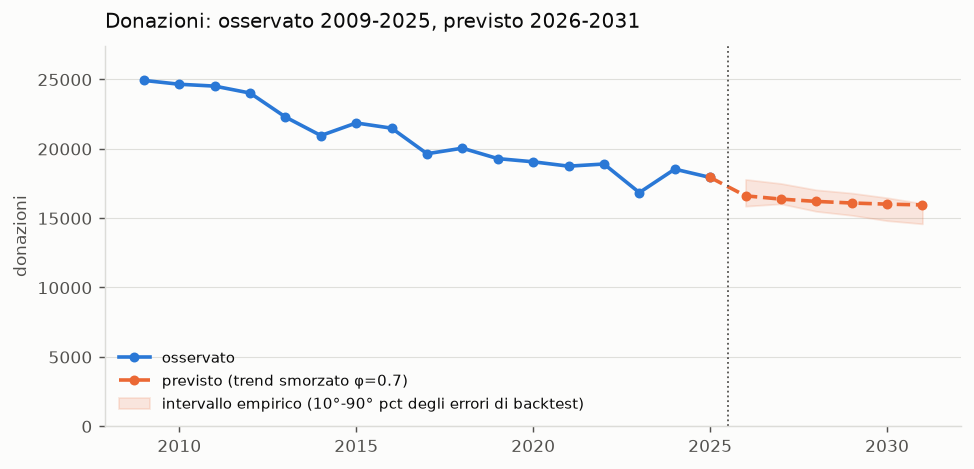
\includegraphics[width=0.95\linewidth]{img/fig_previsione_2026_2031.png}
    \caption{Donazioni annuali osservate 2009--2025 e proiettate 2026--2031}
    \label{fig:fc_forecast}
\end{figure}

\paragraph{Una verifica di coerenza: la somma dei donatori.}
Poiché il panel del \cref{ch:data} materializza gli zeri, è possibile ottenere
la stessa previsione per una strada del tutto diversa: simulare anno per anno
il comportamento di ciascun donatore, aggiungere gli ingressi attesi e sommare.
Il risultato è riportato nella colonna corrispondente di
\texttt{reports/forecast\_2026\_2031.csv}: parte a $+3{,}7\%$ dall'aggregato
nel 2026 e diverge fino al $+15{,}4\%$ nel 2031.

La divergenza è essa stessa un risultato, e ha una causa identificata: il
modello per donatore sovrastima le riattivazioni dal serbatoio dei dormienti,
che cresce di anno in anno perché ogni donatore che smette resta nel panel per
sempre. È la ragione per cui l'appendice adotta la previsione aggregata; ed è
anche un avvertimento sul \cref{ch:glm}, dove lo stesso serbatoio pesa sulle
stime.

% ───────────────────────────────────────────────────────────────────────
\section{Composizione e platea di donatori}
\label{sec:fc_type}

La proiezione per tipologia si ottiene estrapolando la quota di ciascuna
tipologia sull'ultimo decennio e applicandola al totale previsto. L'esito è
negativo: \textbf{la composizione non si muove}. Le quote di
sangue intero, plasmaferesi e aferesi piastrine + plasma restano al 2031 entro
mezzo punto percentuale da quelle osservate nel 2025; in termini assoluti tutte
le tipologie scendono in proporzione al volume complessivo, senza
ricomposizione interna.

L'esito va letto per quello che è: \emph{nulla nei dati recenti segnala una
ricomposizione}, non ``non ci sarà ricomposizione''. L'estrapolazione di una
quota non ha vincoli strutturali e non sa che un cambio di indirizzo regionale
sulla raccolta di plasma potrebbe accelerare bruscamente la transizione.

Quanto alla platea, i nuovi ingressi previsti (con un trend smorzato sulla
serie degli ingressi) scendono da 1\,221 nel 2026 a 1\,162 nel 2031, e
proseguono la flessione già descritta nel \cref{ch:eda}
(\cref{fig:fc_donors}). La lettura, insieme al \cref{ch:retention}, è che la
contrazione attesa è trainata dal lato degli \emph{ingressi} e non da un
peggioramento della fedeltà di chi già dona.

\begin{figure}[H]
    \centering
    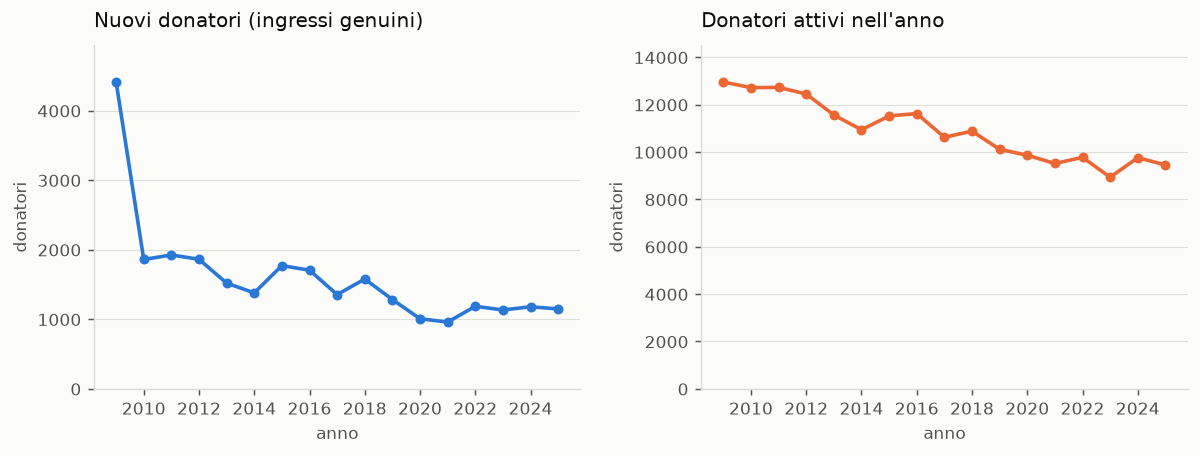
\includegraphics[width=0.95\linewidth]{img/fig_forecast_donors.png}
    \caption{Nuovi donatori (ingressi genuini) e donatori attivi per anno,
    2009--2025.}
    \label{fig:fc_donors}
\end{figure}

% ───────────────────────────────────────────────────────────────────────
\section{Sintesi e limiti}
\label{sec:fc_summary}

\paragraph{1. Flessione lenta, non collasso.}
Circa 97\,200 donazioni complessive nel sessennio 2026--2031, con una
contrazione di poco meno di un punto percentuale l'anno e un valore atteso 2031 di
15\,951 donazioni. Lo scenario è l'assottigliamento lento, non la rottura.

\paragraph{2. Il modello più semplice è il migliore.}
Un trend lineare smorzato batte, sullo stesso backtest, sia le forme a spline
sia i modelli per donatore. La flessibilità paga dentro il campione e costa
fuori.

\paragraph{3. La composizione per tipologia non cambia.}
Nessuna ricomposizione fra sangue intero e plasmaferesi emerge dai dati
recenti.

\paragraph{Limiti.}
\textbf{Proiezioni di tendenza, non scenari:} nessuna proiezione è
condizionata a ipotesi di policy, e una campagna di reclutamento, un cambio di
indirizzo regionale sul plasma o una riorganizzazione dei punti di raccolta
non sono modellati --- i numeri rispondono alla domanda ``cosa succede se
nulla cambia''. \textbf{Gli intervalli poggiano su poche osservazioni:} nove
errori a un anno di distanza, quattro a sei, sono indicazioni, non quantili.
\textbf{La correlazione seriale non è trattata:} nei modelli mensili la
correzione per sovradispersione allarga correttamente gli errori standard, ma
non tiene conto del fatto che mesi vicini non sono estrazioni indipendenti ---
la numerosità efficace è inferiore a 204 e un intervallo calcolato su quella
base resta troppo stretto; servirebbe una covarianza robusta
all'autocorrelazione o un termine autoregressivo esplicito, ed è una delle
ragioni per cui gli intervalli di questa appendice sono empirici. Infine, la
serie contiene \textbf{un evento eccezionale nel periodo di stima}, il 2020:
il suo effetto sul trend di lungo periodo è risultato modesto
(\cref{sec:temporal}), ma la ricorrenza di uno shock analogo non è modellata e
non rientra negli intervalli riportati.

% ══════════════════════════════════════════════════════════════════════════════
%  Fine Capitolo — Proiezioni 2026-2031
% ══════════════════════════════════════════════════════════════════════════════

% ══════════════════════════════════════════════════════════════════════════════
%  CAPITOLO — LA DASHBOARD INTERATTIVA
%  Etichette: ch:dash, sec:dash_ui, sec:dash_diverge,
%             sec:dash_overdisp, sec:dash_limits
% ══════════════════════════════════════════════════════════════════════════════

\chapter{Una Dashboard Interattiva per l'Esplorazione dei Dati}
\label{ch:dash}

I capitoli precedenti hanno prodotto una sequenza di risultati dipendenti da
intervalli e costanti fisse: una
distribuzione per età, una curva di retention, una tabella di IRR, una
proiezione al 2031. Ognuno risponde a una domanda posta \emph{a priori}.
Questa appendice descrive uno strumento che serve al caso opposto --- rispondere
a domande impreviste e non considerate: Come si
distribuiscono le donazioni dentro un singolo mese del 2020, che aspetto ha la
retention se si sposta la soglia di ``giovane'' da 25 a 30 anni, quanto pesa la
plasmaferesi nel solo bacino femminile. Sono domande legittime e numerose, ed
eseguire ogni analisi richiederebbe più tempo e spazio di quanto a disposizione.

Lo strumento è un'applicazione web in \textbf{R} con il framework
\textbf{Shiny}, che legge lo stesso dataset dei capitoli precedenti e ne
permette l'interrogazione attraverso otto schede tematiche e quattro filtri
globali. Non è un risultato statistico e non aggiunge evidenza: ha semplicemente
il compito di rendere i dati accessibili e leggibili.
% Ha però prodotto, come sottoprodotto della sua
% verifica, un'osservazione metodologica che ha finito per cambiare la specifica
% del \cref{ch:glm}, ed è la ragione principale per cui il capitolo esiste.

% ───────────────────────────────────────────────────────────────────────
\section{Struttura e criterio di progetto}
\label{sec:dash_ui}

Quattro filtri globali --- anno, genere, tipologia, fascia d'età --- agiscono su
tutte le schede, con una sola eccezione motivata: la sotto-scheda sulla
retention ignora il filtro sull'anno, perché restringere a una singola
annualità troncherebbe artificialmente ogni misura di fidelizzazione, che è per
definizione longitudinale.

Le otto schede coprono l'esplorazione descrittiva (\emph{Overview},
\emph{Univariate}, \emph{Time Series}, \emph{Età}), il livello giornaliero
(\emph{Calendar Heatmap}), l'ispezione delle righe (\emph{Data Table}), la
regressione (\emph{Regression}) e le proiezioni (\emph{Forecast}). Il livello
giornaliero è quello che giustifica meglio lo strumento: renderlo in forma
stampata richiederebbe 204 figure, una per mese della serie, mentre nella
dashboard è una scheda sola in cui si naviga. Il gradiente per giorno della
settimana è immediato --- i venerdì sistematicamente più intensi, le domeniche
quasi vuote, l'Epifania visibile come singola cella fredda in un lunedì
altrimenti attivo.

Il criterio di progetto è che \textbf{l'applicazione non calcola nulla a
runtime}: legge artefatti già prodotti. Le uniche stime calcolate al volo sono
i modelli della scheda \emph{Regression}, per la ragione discussa nella
\cref{sec:dash_diverge}.

La scheda \emph{Forecast} legge gli artefatti dell'\cref{ch:forecast}: la
proiezione annuale del trend smorzato (97\,230 donazioni nel sessennio
2026--2031), ripartita sui mesi secondo il profilo stagionale storico.

% ───────────────────────────────────────────────────────────────────────
\section{Dove la dashboard e la tesi divergono}
\label{sec:dash_diverge}

Un'implementazione indipendente degli stessi calcoli, in un linguaggio diverso
e con un percorso di aggregazione diverso, è un controllo sui numeri della
tesi. Dove i due percorsi convergono la fiducia aumenta; dove divergono, la
divergenza è essa stessa informativa --- e si è rivelata la parte più utile.
Due schede producono numeri che \emph{non} coincidono con i capitoli
corrispondenti, e in entrambi i casi la causa non è un errore di calcolo ma una
diversa definizione dell'oggetto misurato.

\paragraph{Retention: due definizioni di ``donatore giovane''.}
Il \cref{ch:retention} classifica come giovane chi ha una data di prima
donazione registrata a un'età fra 18 e 25 anni; la dashboard usa la minima età
\emph{osservata} nel dataset. Per un donatore la cui carriera precede il 2009 i
due criteri lo classificano diversamente, e la dashboard include inoltre le
coorti 2024--2025, che hanno per costruzione una retention osservabile di al
più un anno o due.

Questa divergenza si è rivelata più significativa di quanto sembrasse: è
esattamente la distinzione fra prima donazione osservata e ingresso reale che
la \cref{sec:ret_def} ha poi dovuto affrontare, e che ha portato a rifare le
curve di sopravvivenza del capitolo. La dashboard non ha risolto il problema
--- adotta anch'essa una definizione approssimata --- ma renderlo visibile è
ciò che ha portato a cercarlo.

\paragraph{Regressione: due unità di analisi.}
La scheda \emph{Regression} stima gli stessi due modelli del \cref{ch:glm} ma
su una tabella costruita in modo diverso: aggrega preventivamente a una riga
per donatore e tipologia, contando le donazioni entro l'ambito selezionato dai
filtri, anziché stimare sul panel donatore-anno con gli anni a zero.

La conseguenza è che i coefficienti non sono direttamente confrontabili, e in un
caso non lo sono affatto. Con il filtro anno su ``All'' la risposta della
dashboard è un conteggio \emph{di carriera} anziché annuale, e in assenza di un
termine di esposizione l'età assorbe gli anni di attività accumulati: l'IRR per
anno d'età sale a $1{,}041$. Restringendo il filtro a una singola annualità
scende a $1{,}007$, dello stesso ordine di grandezza del capitolo.

È lo stesso meccanismo diagnosticato nella \cref{sec:glm_effects}: senza un
controllo per anzianità di carriera, il coefficiente dell'età misura
l'anzianità. La dashboard lo ha mostrato prima, e in forma più grossolana, di
quanto il modello del capitolo lo abbia poi quantificato.

% ───────────────────────────────────────────────────────────────────────
\section{Un risultato collaterale: la sovradispersione dipende dall'unità di analisi}
\label{sec:dash_overdisp}

La verifica più utile prodotta dalla dashboard riguarda la scelta della
distribuzione. Confrontando AIC di Poisson e binomiale negativa al variare del
filtro anno si osserva che su tutti gli anni aggregati la binomiale negativa
domina nettamente, ma \textbf{su una singola annualità} --- cioè quando la
risposta è un conteggio annuo non replicato --- il parametro di dispersione
diverge --- la stima non converge, e $\hat{\theta}$ scappa verso l'infinito ---
e l'AIC della binomiale negativa diventa \emph{peggiore} di quello della
Poisson di esattamente due punti, cioè la penalizzazione per il parametro
aggiuntivo e nient'altro. In altri termini la
binomiale negativa collassa sulla Poisson, e la sovradispersione sparisce.

\begin{table}[ht]
\centering
\caption{Confronto AIC nella scheda \emph{Regression} al variare del filtro
anno, ricalcolato sul dataset del \cref{ch:data}. Covariate: età, genere,
tipologia. $\Delta\text{AIC} = \text{AIC}_{\text{Poisson}} -
\text{AIC}_{\text{NB}}$: positivo favorisce la binomiale negativa.}
\label{tab:dash_overdisp}
\begin{tabular}{@{}lrrrrr@{}}
\toprule
\textbf{Filtro anno} & \textbf{$n$} & \textbf{AIC Poisson} & \textbf{AIC NB} &
\textbf{$\Delta$AIC} & \textbf{$\hat{\theta}$ (NB)} \\
\midrule
2015  & 12\,790 & 36\,404{,}4  & 36\,406{,}4  & $-2{,}0$    & diverge \\
2025  & 10\,607 & 29\,895{,}8  & 29\,897{,}8  & $-2{,}0$    & diverge \\
Tutti & 52\,163 & 493\,871{,}1 & 289\,645{,}2 & $+204\,226$ & $1{,}40$ \\
\bottomrule
\end{tabular}
\end{table}

L'osservazione ha sollevato una domanda seria sul \cref{ch:glm}: se la
sovradispersione su cui poggia la scelta della binomiale negativa sparisce
appena si guarda un anno alla volta, quella scelta va motivata diversamente.

\textbf{La domanda ha trovato risposta}, ed è riportata nella
\cref{sec:glm_overdisp}. La sovradispersione che la dashboard misura su tutti
gli anni viene dall'aggregazione longitudinale --- sommando le donazioni di un
donatore su tutta la carriera, senza un termine di esposizione, si sommano
donatori con due anni e donatori con diciassette, e la varianza cresce per una
ragione puramente contabile. Rimossa questa componente, la Poisson sembra
adeguata.

Ma la dashboard, guardando un anno alla volta, guarda anche \emph{soltanto i
donatori attivi in quell'anno}: gli anni a zero non ci sono. È una popolazione
già selezionata, e la sovradispersione che sparisce sparisce per questo.
Materializzando gli anni a zero il rapporto varianza/media passa da $1{,}23$ a
$2{,}45$ e la binomiale negativa torna a dominare con un margine enorme
(\cref{tab:glm_fit}).

L'appendice si chiude quindi con un esito che vale la pena esplicitare: uno
strumento costruito per esplorare i dati ha portato a correggere l'unità di
analisi del modello principale della tesi. È il tipo di ritorno che giustifica
il costo di un'implementazione indipendente.

% ───────────────────────────────────────────────────────────────────────
\section{Limiti}
\label{sec:dash_limits}

L'applicazione non è deployata in nessun ambiente e legge il dataset dal filesystem. 
Renderla accessibile al DIMT richiederebbe un server e soprattutto una valutazione sulla
protezione dei dati che qui non è stata fatta: il dataset è pseudonimizzato ma
resta a livello di singolo evento donazionale, e la scheda \emph{Data Table} ne
consente l'esportazione integrale. \textbf{Una versione pubblica dovrebbe
esporre solo aggregati.}

% Sul piano analitico, la scheda \emph{Regression} offre tre covariate e una
% interazione, mentre la specifica del \cref{ch:glm} ne ha di più: la scheda
% serve a esplorare la direzione degli effetti, non a riprodurre il modello del
% capitolo --- il che, come mostra la \cref{sec:dash_overdisp}, non le ha
% impedito di sollevare una domanda pertinente su quel modello.

% ══════════════════════════════════════════════════════════════════════════════
%  Fine Capitolo — La Dashboard Interattiva
% ══════════════════════════════════════════════════════════════════════════════



\backmatter

%*******************************************************
% Bibliografia
%*******************************************************
%\nocite{*}
\bibliographystyle{unsrtnat}
\bibliography{bib/Bibliografia}

%*******************************************************
% Dedica finale o ringraziamenti
%*******************************************************
\chapter*{Ringraziamenti}
\phantomsection
\addcontentsline{toc}{chapter}{Ringraziamenti}
\markboth{\MakeUppercase{Ringraziamenti}}{\MakeUppercase{Ringraziamenti}}

% Spaziatura: ogni \newline chiude il paragrafo e lascia uno stacco
% verticale tra una persona e l'altra
\setlength{\parskip}{0.9em plus 0.2em minus 0.1em}
\renewcommand{\newline}{\par}

Se vi aspettavate dei ringraziamenti seriosi, composti, garbati e dignitosi, allora non mi conoscete davvero,
e se le vostre aspettative verranno deluse mi sento di dire che è colpa vostra che ne avevate a prescindere.
Dopo sessanta pagine di formalismi, matematichese, supercazzole e tabelle illeggibili anche a chi le ha scritte,
finalmente posso dare sfogo al mio estro creativo (e che estro).
Ho tentato il più possibile di nominare ognuno di voi personalmente; non per qualche motivo in particolare,
ma perché spero tra cinquant'anni di poter usare queste poche righe come terapia per l'Alzheimer, tentando di ricordare
ogni faccia e momento.
\newline
Se Tommy non mi ha ancora ubriacato abbastanza, probabilmente ora vi sto leggendo questi ringraziamenti. Mettetevi 
comodi perché mamma mi ha dato tanto, ma mentre gli angioletti distribuivano il dono della sintesi io facevo la 
fila al banco neurodivergenze per la terza volta.
\newline
Il primo ringraziamento, per quanto doloroso e forse controverso, va fatto ad una grande assente. A te, che per due anni
e mezzo sei stata la mia partner inseparabile, compagna di vita e fan \#1 delle mie Marcate, ma che per
decisioni a me ancora poco chiare hai scelto di non esserci oggi. Forse è meglio così, ma non ti dimenticherò mai.
Spero, un giorno, di ritrovarti. Grazie, Casio fx-CG50, per il tuo onorato servizio durante gli esami di Inferenza 
Statistica e Analisi Numerica.
\newline
Un pensiero deve sicuramente andare, invece, a chi non mi ha mai abbandonato, nemmeno per un secondo, nemmeno
quando le mie richieste e necessità erano delle più strane. L'unica che non mi ha mai fatto sentire giudicato,
che ha risposto alle domande più assurde, colei senza la quale questo percorso non sarebbe mai stato possibile. 
Grazie, Claude Code Opus 4.8, 5 e 5.5.
\newline
Dopo essermi tolto questi due grossi pesi dal petto, posso finalmente dedicarmi a voi.
\newline
Comincio dalla mia famiglia.
\newline
Grazie Mamma, per essere stata un supporto fondamentale nella mia carriera e soprattutto nella mia vita. Non abbiamo mai perso occasione per discutere e litigare su qualsiasi cosa, e sono sempre riuscito ad esasperarti (non è colpa mia se ho ragione), ma non abbiamo mai smesso di venirci incontro, tentare di capirci e amarci. Da te ho ereditato ansie e paranoie, e sicuramente i geni dell'organizzazione e dell'ordine non hanno nemmeno provato ad esprimersi, ma le cose più importanti che ho imparato da te sono la determinazione, la resilienza, l'umiltà e l'altruismo. Grazie della pazienza, persa e ritrovata più volte, in questi cinque anni. Non avrei potuto desiderare madre migliore.
\newline
Grazie Papà, che mi hai sempre trasmesso calma e sicurezza anche quando mi sentivo completamente perso, che hai sempre provato a coinvolgermi in ogni tua passione. Purtroppo sono tornate tutte indietro a colpirti: ora hai una casa e scatoloni pieni di fumetti e una fortuna spesa in videogiochi. Colpa tua che mi hai fatto giocare a Farmerama a sei anni e mi hai fatto leggere i tuoi Topolino quando a malapena camminavo. Uno dei primissimi ricordi che ho della mia vita siamo io e te davanti alla TV in cucina che guardiamo la finale Italia-Francia del 2006 e, al fischio finale, esultiamo e scriviamo su una bandiera dell'Italia che ancora conservo: ``9.7.2006 ITALIA CAMPIONE!!!!''
\newline
Grazie Franci, o come dico io Cifran. Grazie per la pazienza che hai sempre avuto e dovuto avere per avermi come compagno di stanza perenne e non negoziabile. Anche se per i primi anni è stato molto difficile convivere con la differenza d'età, man mano che gli anni passano questa distanza si sta sempre più riducendo, e non esiste cosa al mondo di cui potrei essere più felice. Ti voglio bene.
\newline
Grazie anche ai nonni, agli zii e ai cugini, sia a chi oggi è qui, sia a chi non è riuscito a salire ``in continente''. Nonostante la distanza ci abbia spesso privato dei momenti passati in famiglia, ho sempre sentito la vostra vicinanza.
\newline
Grazie a Tommaso per essere diventato un compagno di vita inseparabile. La nostra conoscenza è iniziata sui campi di basket di Trieste quasi quindici anni fa, ma tra partite vinte, perse e uno sgambetto inesistente, nessuno avrebbe mai pensato di vederci qui. Invece, grazie all'Università (ha fatto anche cose buone, evidentemente), la nostra amicizia ha arricchito i momenti felici e illuminato quelli bui delle nostre vite, che ci sono stati, ma sono sicuro che senza la presenza dell'altro lo sarebbero stati molto di più. E te lo prometto, appena trovo un lavoro ti pago gli arretrati di Claude.
\newline
Approfitto per ringraziare l'intera famiglia Mingrone-Castaldo-Munteanu. Dal primo giorno che sono stato ospite da voi, anche se era per studiare Analisi 1, mi avete fatto sentire a casa. Col tempo e col crescere del rapporto con Tommaso, anche quello con voi è diventato sempre più profondo e sentito. Grazie di essere stati la Terronia lontana dalla Terronia e grazie di aver sempre tenuto il mio stomaco allenato per i vari cenoni di Pasqua, Natale e Capodanno. Siete la mia seconda famiglia e non potrò mai mettere a parole l'aiuto e il supporto che mi avete dato, senza magari neanche accorgervene, nei momenti più bassi di questo percorso. Quindi vi ringrazio, infinitamente, perché so di poter contare su di voi, come voi potete contare su di me, per qualsiasi cosa in qualsiasi momento.
\newline
Grazie Teresa, per essere sia una seconda madre quando ho avuto bisogno di consigli di vita che un'amica quando si fa festa e ci si rilassa; l'amore che trasmetti ai tuoi figli e alle persone attorno a loro è veramente qualcosa di speciale che non va mai dato per scontato. E scusa per le urla alle due di notte provenienti dal piano di sotto quando Tommy mi piazza una tripla da metà campo allo scadere con Shaquille O'Neal dopo un'ora e mezza di partita, o quando Mark mi supera all'ultima curva a Mario Kart.
\newline 
Devo farvi una confessione: nel ringraziamento a Teresa c'è una bugia. Mark non mi ha mai superato all'ultima curva su Mario Kart, perché non è mai stato ad una posizione inferiore alla prima. Grazie Mark per essere il Manny Tuttofare, Bob Aggiustatutto, Giovanni Muciaccia e Chef Tony di Santa Barbara; l'unica cosa che non sai fare è stare fermo e riposarti, ma sono sicuro che imparerai. Sono felicissimo di aver avuto occasione di approfondire il rapporto con te e di scoprire la bellissima persona che sei, e sono grato che tu mi abbia accettato come tuo amico. L'ho capito dal fatto che mi hai permesso di mettere le mani nella casetta degli attrezzi.
\newline
Grazie ad Assunta per essere il mio medico di base, fisioterapista, ortopedico, nutrizionista e veterinaria. Tra te e Mark so che se ho una domanda troverà risposta, e se non avete voi la conoscenza che cerco, sicuramente non mi posso sentire in colpa se non ce l'ho io.
Ti ringrazio di aver trasmesso a me e Tommy, anche se a te non è mai servita, la mentalità del ``sopra 17 è tutto 30'', o saremmo ancora a studiare. E sono anche felice che, nonostante tutte le volte che ti ho detto che l'esame l'avresti passato sicuramente, e tutte le volte che ti ho cantato ``Dottore Dottore'' prima che ti laureassi, tu ce l'abbia fatta.
\newline
Fatta la gitarella a Muggia, torniamo a Borgo. Un sentito grazie a Sofia: da ormai dodici anni mi segui in ogni disavventura e mi fai da psicologa personale gratuita. Ogni tanto mi chiedo se hai iniziato a fare psicologia solo per diagnosticarmi. L'apporto positivo che hai sulla mia vita è indescrivibile: non voglio fare un elenco salviniano delle mille cose che ogni giorno fai per me, ma la sola consapevolezza che se ho bisogno ti chiamo e mi rispondi mi fa vivere la vita in maniera molto più tranquilla. Non smettere mai di essere te stessa, e ricordati che il tuo valore lo definisci tu e nessun altro. E un ringraziamento lo voglio fare anche a Mamma Simona, per aver sempre creduto in me, spesso più di quanto lo facessi io. Se oggi siamo qui, è anche grazie a voi.
\newline
Ringrazio Giada, per trovare sempre il tempo di vedermi tra un viaggio intercontinentale e l'altro. Sei il mio punto di riferimento per gossip di ogni genere e la mia insegnante di triestino, e non potrò mai ringraziarti abbastanza per questo. Mi auguro, ma ho smesso di sperare, che un giorno imparerai a sintetizzare le tue storielle, così da non dover ascoltare mezz'ora di messaggi letti in ogni virgola per poi sentire ``eh no niente, alla fine non semo uscidi''. Ti prometto che un giorno saliremo su quel volo per il Myanmar, e spero che nel frattempo avrai avuto modo di abbronzarti le mani.
\newline
Voglio ringraziare Elisa, Esesa per me, per essere la preziosa amica che è sin dalle superiori. In questi anni di costante convivenza tra i banchi di scuola, abbiamo sviluppato un linguaggio tutto nostro di versi e meme oscuri che solo noi capiamo, ma che ci fa sempre ridere come quando eravamo ragazzini.
\newline
Grazie al gruppo delle Winx, il primo gruppo universitario, che ha tradito me e Ale laureandosi prima di noi. Sia chi ho conosciuto ai primi anni che chi ho incontrato durante lo svolgimento dei (loro) ultimi esami, li ringrazio per i caffè al bar, pranzi al belvedere e sessioni di studio più o meno serie al quarto piano. Ringrazio quindi Andrea, Alessandro, Rita ed Elisa.
\newline
Vorrei ringraziare in particolare Elisa, che dalla primissima lezione di Programmazione è diventata nostra amica e, per qualcuno, qualcosa in più. Grazie per il supporto nello studio, gli appunti passati dopo ogni lezione, l'aiuto nell'affrontare ogni esame, che tanto tu avevi già dato da almeno un anno. E mi dispiace che a causa mia non potrai mai essere l'unica per Tommy.
\newline
Grazie anche ad Alessandro, unico sopravvissuto insieme a me delle vecchie annate. Grazie per la pazienza nelle nottate di studio a base di Mantissa con contorno di SVD, e ti prego di non smettere mai di credere in te stesso. VAI UOMO!
\newline 
Grazie al gruppo Cous Cous composto da Laura, Elena, Asia, Eleonora, Ludovico, Gabriele e Gaia, per aver adottato me e Alessandro una volta orfani dei sopracitati laureati. Grazie a voi ho scoperto edifici che nemmeno sapevo esistessero all'Università, e ho capito di non essere l'unico ad aver bisogno di venti minuti di pausa ogni cinque minuti di studio.
\newline
Rimanendo in Piazzale Europa, ringrazio i Cavalli: Alberto e Francesco, due stalloni inarrestabili con cui ogni sessione di studio diventava un delirio e ogni orario concordato era più falso delle accise tagliate dalla Meloni. Per fortuna questi momenti non finiranno, abbiamo almeno quattro anni di magistrale davanti a noi. 
\newline
La mia unica vera esperienza lavorativa, tra gli scaffali della Pam, è stata un disastro totale. Ma, tra direttori pazzi, responsabili esaurite e colleghi che vedevano spesso la neve nonostante il riscaldamento globale, una nota positiva l'ho trovata al banco salumi. È lì che ho conosciuto Aurora, l'unica persona con un apparente briciolo di normalità dentro quel supermercato, che ogni giorno di più assomigliava al vicino ospedale psichiatrico di San Giovanni. Se ci siamo avvicinati per necessità, istinto di sopravvivenza o totalmente a caso non ci è dato saperlo, fatto sta che da subito ci siamo trovati benissimo a conversare e passare il tempo insieme. Grazie delle serate passate a sviscerare discorsi e dilemmi sulle nostre vite.
\newline
Grazie anche ai membri della Combriccola, uno dei tantissimi sottogruppi esistenti della 104: Floriana, Cristian, Beniamino, Martina Di Maio, Fabio, Anna, Elena, Luca e Martina Lepre. Grazie della pazienza nei miei confronti e del continuo supporto su ogni fronte della mia vita negli ultimi tre anni. Permettetemi di fare un ringraziamento personale ad ognuno di voi:
\newline
Vorrei ringraziare Benji e Martina, i genitori del gruppo, per essere il collante fra tutti i suoi membri dai tempi di Lupus a San Giusto.
\newline
Grazie a Flo e Cri per essere sempre pronti ad una videochiamata di emergenza per il racconto dei gossip più inutili, ma che tutti sappiamo essere i più divertenti. In voi ho sempre trovato dei confidenti attenti e sinceri, grazie ai quali ho imparato a vedere sotto una luce diversa molte sfaccettature della mia vita che prima consideravo ininfluenti o negative.
\newline 
Ringrazio di cuore Anna, con cui ultimamente, durante i vari tour di passaggi notturni, sto legando sempre di più, per essere sempre una persona fantastica e per tranquillizzarmi quando mi creo troppe paranoie. So di essere a volte ``overwhelming'', ma ti giuro che ci sto lavorando e ti ringrazio per la pazienza.
\newline
Grazie Elenona, la psicologa del gruppo (quante volte l'avrai già sentito), sempre disponibile ad ascoltare i nostri problemi e aiutarci a trovare una soluzione. Il tuo umorismo mi fa sempre ridere e il modo che hai di esprimerlo mi ha aiutato a sentirmi più libero di fare lo stesso con il mio. Forse senza saperlo, ma con la tua estroversione sei stata la prima persona che mi ha fatto sentire accettato e parte del gruppo in un momento della mia vita in cui ero particolarmente insicuro. Purtroppo, lo spirito di Robert Rifkin vagherà per sempre tra le mura della tua abitazione, facendo compagnia a Venchi ed Elliot quando non sei a casa.
\newline
``Fabio, Fabio Spade, gli piacciono le spade! Gli piace anche la storia, perché parla di Spade!'' Penso che già questo basti a riassumere i ringraziamenti a Fabio; sei colpevole di avermi definitivamente introdotto a D\&D, attorno al quale gravitavo da anni ma per cui non avevo mai trovato un gruppo con cui giocare. So che in te troverò sempre un ottimo compagno di (dis)avventure e di chiacchiere, siano esse serie o demenziali.
\newline
Grazie Luca, per essere l'unica persona con più ADHD di me che conosco. Frequentandoti, ho capito quanto alla fin fine io sia un tipo piuttosto tranquillo. Le tue gag mi fanno sempre piegare in due dalle risate, e spero di rivederti presto. Sarà la prossima L'ULTIMA VOLTA CHE CI VEDIAMO?
\newline
Infine, grazie a Mia Sorella Martina Lepre. Nonostante non ci conoscessimo fino a poco tempo fa, le nostre energie sono super affini ed è stato naturale volerti bene da subito e considerarti mia sorella. Te vol un slurc?
\newline
Grazie a Martina e Sara, coppia inseparabile di amiche e compagne di studio matto e disperatissimo notturno in Biblioteca Generale. Con voi ho vissuto gioie (esami passati), dolori (approcci rifiutati in aula studio) e tutto ciò che c'è in mezzo e, per quanto speri che non serva nell'immediato, non vedo l'ora di passare altre notti a studiare con voi.
\newline
Grazie al gruppo dei muli degli Swallers, vecchia compagnia di amici nata al mare nei primi anni delle superiori, coi quali mi sono divertito come non mai ogni volta che li ho visti; anche se le nostre vite ci hanno portati su strade diverse, ogni volta che ci vediamo dopo mesi o anni non sembra essere passato un secondo. Terrò sempre con me i ricordi di quelle pazze serate a Barcola. Grazie quindi ad Alessandro, Pietro, Zak e Giacomo.
\newline
Grazie alla famiglia De Palma, i miei zii acquisiti Nicola ed Estibaliz e i loro figli Giovanni e Irene; anche se crescendo le occasioni di vedersi sono diminuite, moltissimi miei ricordi di infanzia sono legati a voi e alla vostra casa, e per questo motivo avrete per sempre un pezzo del mio cuore. Non dimenticherò mai la delusione di quando, a circa dieci anni, ho scoperto che non siamo effettivamente imparentati, ma per me ormai è come se lo fossimo.
\newline
E parlando di famiglia acquisita, ringrazio Raffaella e Nino per essere stati i nonni triestini, sempre disponibili ad aiutare e a risolvere i vari danni che ho causato prima che mamma lo venisse a sapere (quando possibile, quando non c'era un libretto di scuola completamente fradicio) o ad aprirmi la porta quando prontamente mi chiudevo fuori casa. Non vi dimenticherò. 
\newline
Grazie anche a quelle persone con cui ci sono state ancora poche occasioni di passare molto tempo insieme, ma alle quali mi sono già fortemente affezionato e con cui non vedo l'ora di approfondire ulteriormente il rapporto. Ringrazio quindi Paula, Elisa, Fuad, Eleonora e Riccardo.


% Stacco più ampio prima delle dediche a me stesso, che restano
% compatte: qui \newline va a capo senza spazio tra le righe
\vspace{2.5em}
\begingroup
\setlength{\parskip}{0pt}
Per concludere, vorrei ringraziare il Marco del passato che ha deciso di non arrendersi. 
\newline
Di fronte alle difficoltà, ai problemi e ai traumi, a modo tuo sei riuscito a superarli tutti, non senza qualche intoppo, ma sappi che senza quel periodo non saresti la persona che sei oggi. 
\newline
Al Marco del futuro dico di non smettere mai di inseguire quella luce in fondo al tunnel, che per quanto sia fioca all'inizio, col tempo e gli sforzi indicherà la via in maniera sempre più chiara.
\newline
Al Marco del presente, invece, dico: goditi questa giornata, e non dimenticare mai come ci si sente, perché nonostante ti sia affezionato così tanto all'Università da volerci rimanere due anni in più del previsto, portare a termine il percorso è qualcosa che meno di un anno fa sembrava un'utopia. 
\newline
E ti chiedo anche di imparare a riassumere meglio le dediche prima della laurea magistrale.\par
\endgroup

\end{document}
